\documentclass[12pt, a4paper]{report}
\usepackage[english]{babel}
\usepackage{titlesec}

\titleformat{\chapter} % command
  [display] % shape
  {\bfseries\huge} % format
  {Chapter \thechapter} % label
  {0pt} % sep
  {} % before-code


\usepackage[T5]{fontenc}
\usepackage{mathptmx}[ptm]
\usepackage{a4wide, amssymb, epsfig, latexsym, array, hhline, fancyhdr}
\usepackage[normalem]{ulem}
%\usepackage{soul}
\usepackage{float}
\usepackage[makeroom]{cancel}
\usepackage{amsmath}
\usepackage{amsthm}
\usepackage{multicol, longtable, amscd}
\usepackage{diagbox}%Make diagonal lines in tables
\usepackage{booktabs}
\usepackage{alltt}
\usepackage[framemethod=tikz]{mdframed}% For highlighting paragraph backgrounds
\usepackage{indentfirst}
\usepackage{caption,subcaption}
\usepackage{svg}
\graphicspath{ {figures/} }
\usepackage{lastpage}
\usepackage[lined,boxed,commentsnumbered]{algorithm2e}
\usepackage{enumerate}
\usepackage{color}
\usepackage{graphicx}% Standard graphics package
\graphicspath{ {figures/} }
\usepackage{array}
\usepackage{tabularx, caption}
\usepackage{tabularray}
\usepackage{multirow}
\usepackage{multicol}
\usepackage{rotating}
\usepackage{graphics}
\usepackage{geometry}
\usepackage{setspace}
\usepackage{epsfig}
\usepackage{tikz}
\usepackage[numbers]{natbib}
\usepackage{subcaption}

\usepackage{dirtree}



\usetikzlibrary{arrows, snakes, backgrounds, calc}
\usepackage[unicode]{hyperref}
\hypersetup{urlcolor=blue,linkcolor=black,citecolor=black,colorlinks=true} 

\usepackage{xcolor}

\definecolor{codegreen}{rgb}{0,0.6,0}
\definecolor{codegray}{rgb}{0.5,0.5,0.5}
\definecolor{codepurple}{rgb}{0.58,0,0.82}
\definecolor{backcolour}{rgb}{0.95,0.95,0.92}

\usepackage{listings}
\lstdefinestyle{mystyle}{
    backgroundcolor=\color{backcolour},   
    commentstyle=\color{codegreen},
    keywordstyle=\color{magenta},
    numberstyle=\tiny\color{codegray},
    stringstyle=\color{codepurple},
    basicstyle=\ttfamily\footnotesize,
    breakatwhitespace=false,         
    breaklines=true,                 
    captionpos=b,                    
    keepspaces=true,                 
    numbers=left,                    
    numbersep=5pt,                  
    showspaces=false,                
    showstringspaces=false,
    showtabs=false,                  
    tabsize=2
}
\lstset{style=mystyle}



\def\thesislayout{	% A4: 210 × 297
	\geometry{
		a4paper,
		total={160mm,240mm},  % fix over page
		left=30mm,
		top=30mm,
	}
}
\thesislayout

%\usepackage{fancyhdr}
\setlength{\headheight}{40pt}
\pagestyle{fancy}
\fancyhead{} % clear all header fields
\fancyhead[L]{
 \begin{tabular}{rl}
    \begin{picture}(25,15)(0,0)
    \put(0,-8){
\includegraphics[width=10mm, height=10mm]{Images/hcmut.png}}
    %\put(0,-8){\epsfig{width=10mm,figure=hcmut.eps}}
   \end{picture}&
	%
\includegraphics[width=8mm, height=8mm]{hcmut.png} & %
	\begin{tabular}{l}
        \textbf{ Ho Chi Minh City University of Technology } \\
        \textbf{ Faculty of Computer Science and Engineering }
	\end{tabular} 	
 \end{tabular}
}
\fancyhead[R]{
	\begin{tabular}{l}
		\tiny \bf \\
		\tiny \bf 
	\end{tabular}  }
\fancyfoot{} % clear all footer fields
\fancyfoot[L]{\scriptsize Capstone Project Report (CO4029) - Academic year 2023 - 2024}
\fancyfoot[R]{\scriptsize  Page {\thepage}/\pageref{LastPage}}
\renewcommand{\headrulewidth}{0.3pt}
\renewcommand{\footrulewidth}{0.3pt}

%%%%%%%%%%%%%%%%%%%%%%%%%%%%%%%%%%%%%%%%%%
% Tạo một môi trường mới cho các bảng đặc tả UC, giúp định dạng kiểu
\newenvironment{usecase_table}[1][Test]
{
\begin{table}[H]
% Left-Right Table padding
    \setlength{\tabcolsep}{6pt}
    \renewcommand{\arraystretch}{1.5}
    % \begin{tabularx}{\textwidth}{bs}
    \def\savedcaption{\caption{#1}}%
    \begin{tabular}{|>{\bfseries} p{0.2\linewidth}|p{0.7\linewidth}|}

}
{
    \end{tabular}
    \savedcaption
\end{table}
}

\newenvironment{usecase_enum}
{
    \begin{enumerate*}[itemjoin={\newline}]
}
{
    \end{enumerate*}
}

\makeatletter
\newenvironment{acknowledgments}{
	\small
	\begin{center}
	  {\bfseries Acknowledgments\vspace{-.5em}\vspace{\z@}}
	\end{center}
	\quotation
  }{}
\makeatother

% Declaration
\makeatletter
\newenvironment{declaration}{
	\small
	\begin{center}
	  {\bfseries Declaration\vspace{-.5em}\vspace{\z@}}
	\end{center}
	\quotation
  }{}
\makeatother

\makeatletter
\newenvironment{abstr}{
        \small
        \begin{center}
	{\bfseries Abstract \vspace{-.5em}\vspace{\z@}}
        \end{center}
        \quotation
    }{}
\makeatother

\makeatletter
\newenvironment{abstrsss}{
        \small
        \begin{center}
	{\bfseries Abstractss \vspace{-.5em}\vspace{\z@}}
        \end{center}
        \quotation
    }{}
\makeatother
%%%%%%%%%%%%%%%%%%%%%%%%%%%%%%%%%%%%%%%%%%%%%%5
\setcounter{secnumdepth}{4}
\setcounter{tocdepth}{3}
\makeatletter
\newcounter {subsubsubsection}[subsubsection]
\renewcommand\thesubsubsubsection{\thesubsubsection .\@alph\c@subsubsubsection}
\newcommand\subsubsubsection{\@startsection{subsubsubsection}{4}{\z@}%
                                     {-3.25ex\@plus -1ex \@minus -.2ex}%
                                     {1.5ex \@plus .2ex}%
                                     {\normalfont\normalsize\bfseries}}
\newcommand*\l@subsubsubsection{\@dottedtocline{3}{10.0em}{4.1em}}
\newcommand*{\subsubsubsectionmark}[1]{}
\makeatother



\everymath{\color{black}}%make in-line maths symbols blue to read/check easily

\sloppy
\captionsetup[figure]{labelfont={small,bf},textfont={small,it},belowskip=-1pt,aboveskip=-9pt}
%space removed between caption, figure, and text
\captionsetup[table]{labelfont={small,bf},textfont={small,it},belowskip=-1pt,aboveskip=7pt}
\setlength{\floatsep}{5pt plus 2pt minus 2pt}
\setlength{\textfloatsep}{5pt plus 2pt minus 2pt}
\setlength{\intextsep}{10pt plus 2pt minus 2pt}


% Declare a variable named Proc using \newcommand
\newcommand{\Proc}{Assoc. Prof. Dr. Lê Hồng Trang }

\newcommand{\Uni}{Ho Chi Minh University - Vietnam National Unversity, Ho Chi Minh City}

\renewcommand{\labelitemi}{\normalfont\bfseries\textendash}
\renewcommand{\labelitemii}{\textbullet}
\renewcommand*\baselinestretch{1.5}\selectfont


\thesislayout

\begin{document}

\begin{titlepage}
    
\begin{tikzpicture}[remember picture, overlay]
        \draw[line width = 4pt] ($(current page.north west) + (1.0in,-0.5in)$) rectangle ($(current page.south east) + (-0.4in,0.5in)$);
        \draw[line width=1.5pt]
        ($ (current page.north west) + (1.05in,-0.55in) $)
        rectangle
        ($ (current page.south east) + (-0.45in,0.55in) $);
    \end{tikzpicture}

    \begin{center}
        \large \textbf{VIETNAM NATIONAL UNIVERSITY, HO CHI MINH CITY} \\
        \large \textbf{HO CHI MINH UNIVERSITY OF TECHNOLOGY} \\
        \large \textbf{FACULTY OF COMPUTER SCIENCE AND ENGINEERING}
    \end{center}

    \begin{figure}[h!]
        \begin{center}
            
\includegraphics[width=5cm]{Images/hcmut.png}
        \end{center}
    \end{figure}

    \begin{center}
        {\textbf{\Large CAPSTONE PROJECT REPORT}}\\
        \vspace{1cm}
        \textbf{\LARGE BUILDING AN INTEGRATED DATABASE}\\
        \textbf{\LARGE FOR SHORT TERM FORECASTING SYSTEMS}\\
        \textbf{\LARGE IN HYDRO-METEOROLOGY}\\
        \vspace{0.3cm}
        {\Large Major: Computer Science}\\
    \end{center}

    \vspace{1cm}
    \begin{table}[H]
        \resizebox{\textwidth}{!} {
            \begin{tabular}{rll}
                \hspace{4 cm}
                 & \textbf{\Large THESIS COMMITTEE:} & \textbf{\Large Council 9}                   \\
                 & \textbf{\Large SUPERVISORS:}      & \textbf{\Large Lê Hồng Trang}               \\
                 & \textbf{\Large }                  & \textbf{\Large Trương Quỳnh Chi}            \\
                 & \textbf{\Large REVIEWER:}         & \textbf{\Large Trương Quỳnh Chi}            \\
                 &                                   & \textbf{---o0o---}                          \\
                 & \textbf{\Large STUDENT 1:}        & \textbf{\Large Trần Hà Tuấn Kiệt (2011493)} \\
                 & \textbf{\Large STUDENT 2:}        & \textbf{\Large Nguyễn Đức Thuỵ (2012158)}
            \end{tabular}
        }
    \end{table}
    \vspace{1cm}

    \begin{center}
        {\large Ho Chi Minh City, \the\month/\the\year}
    \end{center}
\end{titlepage}


\newpage

\begin{declaration}

    We guarantee that this research is our own, conducted under the supervision
 and guidance of Assoc. Prof. Dr. Lê Hồng Trang. The result of our research is
 legitimate and has not been published in any form prior to this. All materials
 used within this research are collected by ourselves, by various sources and
 are appropriately listed in the references section. In addition, within this
 research, we also used the results of several other authors and organizations.
 They have all been aptly referenced. In any case of plagiarism, we stand by our
 actions and are to be responsible for it. Ho Chi Minh City University of
 Technologytherefore is not responsible for any copyright infringements
 conducted within our research.

    \begin{flushright}

        \begin{tabular}{@{}c@{}} Ho Chi Minh City, \today \\
            \textbf{Team Members}    \\
            Trần Hà Tuấn Kiệt        \\
            Nguyễn Đức Thuỵ
        \end{tabular}

    \end{flushright}
\end{declaration}

\newpage

%-  Lời cảm ơn/ Lời ngỏ
\begin{acknowledgments}

    We, the research group consisting of two members, would like to send our
    thanks toward everyone who has contributed to the success of this thesis.


    First and foremost, we would like to express our gratitude to \Proc. The
    dedication and extensive knowledge of our supervisor not only guided us
    through the challenges of the project but also helped us develop research
    skills and critical thinking.

    We also want to extend special thanks to all the friends, colleagues, and
    family who supported us throughout the research process. The input and
    opinions of everyone enriched the content and quality of the project.

    Last, but certainly not least, we appreciate each other - research partners
    accompanying us in every step of the project. Our collaboration and joint
    contributions have resulted in a product that we take pride in.

    We believe that this project marks a significant step in our development and
    could not have been achieved without the support and contributions of
    everyone involved.


\end{acknowledgments}
\newpage
%-  Tóm tắt LV
\begin{abstr}
    In this document, we introduce a comprehensive proposal to integrate,
    coordinate, and monitor meteorological and hydrological data in Vietnam. The
    proposed system can serve as a foundation for building a national database
    specializing in meteorological information.

    To clarify our proposal, we have built a comprehensive pilot version, in
    which we have simulated the process of collecting and transmitting data from
    the weather station at Nha Be. At the same time, we focused on the process
    of converting and organizing data storage to ensure transparency and optimal
    performance in information processing.
    
    This research is a manifestation of significant efforts in optimizing the
    management of meteorological data in Vietnam. The proposed system not only
    addresses the challenges of integration and coordination but also lays the
    foundation for a robust national database, serving the diverse needs of
    research and applications in the field of meteorology.

    
\end{abstr}




%\thispagestyle{empty}
% \chapter*{Work Assignment}
% \begin{table}[H]
%     \centering
%     \renewcommand{\arraystretch}{1.5}
%     \begin{tabular}{|c|c|c|l|}
%         \hline
%         \textbf{No.}       & \textbf{Full name}                 & \textbf{Student ID}      & \textbf{Work Assignment}                     \\
%         \hline
%         %%%%%Student 1%%%%%%%%%%%
%         \multirow{4}{*}{1} & \multirow{4}{*}{Trần Hà Tuấn Kiệt} & \multirow{4}{*}{2011493} & - Exploratory Data Analysis                  \\
%                            &                                    &                          & - System proposal and architecture           \\
%                            &                                    &                          & - Research and Develop with new technologies \\
%                            &                                    &                          & - Implement system endpoints                 \\
%         \hline
%         %%%%%Student 2%%%%%%%%%%%
%         \multirow{4}{*}{2} & \multirow{4}{*}{Nguyễn Đức Thuỵ}   & \multirow{4}{*}{2012158} & - Exploratory Data Analysis                  \\
%                            &                                    &                          & - System proposal and architecture           \\
%                            &                                    &                          & - Research and Develop with new technologies \\
%                            &                                    &                          & - Implement data processing flows            \\
%         \hline
%     \end{tabular}
% \end{table}
% \newpage

% Revert title name back to English
\renewcommand{\contentsname}{Table of Contents}
\renewcommand{\listfigurename}{List of Figures}
\renewcommand{\listtablename}{List of Tables}
\renewcommand{\bibname}{References}
\renewcommand{\figurename}{Figure}

\tableofcontents
\newpage

%\thispagestyle{empty}
\listoffigures
\listoftables

% \renewcommand\thechapter{Chapter \arabic{chapter}}

\chapter{Introduction}
\section{Problem statement}

In recognizing the need for National Meteorological Services (NMHSs) to improve
their climate data and monitoring services, there is a deliberate focus on those
aspects of climate data management wishing to make the transition to a modern
climate database management system and, just as important, on what skills,
systems and processes need to be in place to ensure that operations are
sustained. In the context of the ever-growing complexity of climate change, the
task of creating an integrated database for short-term forecasting systems in
the fields of meteorology and hydrology poses a considerable challenge. The
question at hand is how we can optimize the management of weather information
from multiple sources and store it efficiently in a database. This optimization
is crucial to ensure the provision of synchronized and high-quality information
to support forecasting systems.

\section{Motivation}


Information about the weather has been recorded in manuscript form for many
centuries. The early records included notes on extreme and, sometimes,
catastrophic events and also on phenomena such as the freezing and thawing dates
of rivers, lakes and seas, which have taken on a higher profile with recent
concerns about climate change.

Specific journals for the collection and retention of climatological information
have been used over the last two or three centuries (WMO 2005). The development
of instrumentation to quantify meteorological phenomena and the dedication of
observers to maintaining methodical, reliable and well-documented records paved
the way for the organized management of climate data. Since the 1940s,
standardized forms and procedures gradually became more prevalent and, once
computer systems were being used by NMHSs, these forms greatly assisted the
computerized data entry process and consequently the development of computer
data archives. The latter part of the twentieth century saw the routine exchange
of weather data in digital form and many meteorological and related data centers
took the opportunity to directly capture and store these in their databases.
Much was learned about automatic methods of collecting and processing
meteorological data in the late 1950s, a period that included the International
Geophysical Year and the establishment of the World Weather Watch. The WMO’s
development of international guidelines and standards for climate data
management and data exchange assisted NMHSs in organizing their data management
activities and, less directly, also furthered the development of regional and
global databases. Today, the management of climate records requires a systematic
approach that encompasses paper records, microfilm/microfiche records and
digital records, where the latter include image files as well as the traditional
alphanumeric representation.

Before electronic computers, mechanical devices played an important part in the
development of data management. Calculations were made using comptometers, for
example, with the results being recorded on paper. A major advance occurred with
the introduction of the Hollerith system of punch cards, sorters and tabulators.
These cards, with a series of punched holes recording the values of the
meteorological variables, were passed through the sorting and tabulating
machines enabling more efficient calculation of statistics. The 1960s and 1970s
saw several NMHSs implementing electronic computers and gradually the
information from many millions of punched cards was transferred to magnetic
tape. These computers were replaced with increasingly powerful mainframe systems
and data were made available online through developments in disk technology.

Aside from advances in database technologies, more efficient data capture was
made possible through the mid-to-late 1990s with an increase in automatic
weather stations (AWSs), electronic field books (i.e. on-station notebook
computers used to enter, quality control and transmit observations), the
Internet and other advances in technology. Not surprisingly, there are a number
of trends already underway that suggest there are many further benefits for
NMHSs in managing data and servicing their clients. The Internet is already
delivering greatly improved data access capabilities and, providing security
issues are managed, we can expect major opportunities for data managers in the
next five to ten years. In addition, Open Source7 relational database systems
may also remove the cost barriers to relational databases for many NMHSs over
this period.

\section{Project Goal}

It is essential that both the development of climate databases and the
implementation of data management practices take into account the needs of the
existing, and to the extent that it is predictable, future data users. While at
first sight this may seem intuitive, it is not difficult to envisage situations
where, for example, data structures have been developed that omit data important
for a useful application or where a data centre commits too little of its
resources to checking the quality of data for which users demand high quality.

In all new developments, data managers should either attempt to have at least
one key data user as part of their project team or undertake some regular
consultative process with a group of user stakeholders. Data providers or data
users within the organization may also have consultative processes with end
users of climate data (or information) and data managers should endeavour to
keep abreast of both changes in needs and any issues that user communities have.
Put simply, data management requires awareness of the needs of the end users.

At present, the key demand factors for data managers are coming from climate
prediction, climate change, agriculture and other primary industries, health,
disaster/emergency management, energy, natural resource management (including
water), sustainability, urban planning and design, finance and insurance. Data
managers must remain cognizant that the existence of the data management
operation is contingent on the centre delivering social, economic and
environmental benefit to the user communities it serves. It is important,
therefore, for the data manager to encourage and, to the extent possible,
collaborate in projects which demonstrate the value of its data resource. Even
an awareness of studies that show, for example, the economic benefits from
climate predictions or the social benefits from having climate data used in a
health warning system, can be useful in reminding senior NMHS managers or
convincing funding agencies that data are worth investing in. Increasingly,
value is being delivered through integrating data with application models (e.g.
crop simulation models, economic models) and so integration issues should be
considered in the design of new data structures.

\section{Project Scope}

This project focuses on Ho Chi Minh City, a sprawling metropolis with a distinct
climate that significantly impacts the daily lives of its residents. To provide
the most valuable weather insights, we will implement a two-pronged approach.

Firstly, We will conduct research and collect data from the meteorological and
hydrological monitoring stations in the city to ensure diversity and
representation of local weather conditions. At the same time, we will proceed
with preprocessing and standardizing the data to ensure accuracy and consistency
of the dataset. Based on what we have collected, we will populate the data to
proper formats and structures.

Secondly, this project entails the development of a comprehensive data platform.
This platform will integrate a central database, designed to efficiently store
and manage weather information from diverse sources. By consolidating these
disparate data streams, we aim to create a unified and dependable resource for
weather data. This platform is anticipated to significantly enhance the workflow
of end-users and will be built with scalability in mind to accommodate future
growth in data volume and user demand.

\section{Stakeholders}

\subsection{The National Center for Hydro-meteorological Forecasting}

The National Center for Hydrometeorological Forecasting (NCHMF), abbreviated for
"Trung tâm Dự báo khí tượng thuỷ văn quốc gia" \ in Vietnamese, is an
organizational unit under the General Department of Meteorology and Hydrology,
Ministry of Natural Resources and Environment\cite{NMHS}. The National
Hydro-Meteorological Forecasting Center has several crucial missions, including
the establishment and presentation of standards and technical regulations for
meteorological and hydrological forecasting, the operation of the national
forecasting and warning system, monitoring and reporting on weather conditions
and climate change, issuing and disseminating forecast bulletins and warnings,
and participating in international meteorological agreements. Additionally, the
center is responsible for conducting research, application, and technology
transfer related to forecasting and warning, and implementing administrative
reform and anti-corruption measures. These key missions contribute significantly
to the center's role in ensuring public safety and providing timely essential
meteorological and hydrological information.

\subsection{Nha Be Weather Radar Station}

The Nha Be weather radar station is located on Nguyen Van Tao Street, Long Thoi
Commune, Nha Be District, Ho Chi Minh City. This radar station has been in
operation since 2004 and is managed by the Southern Region Hydro-Meteorological
Center. Its mission is to monitor and supervise weather phenomena within a
radius of 480 km from the center of Ho Chi Minh City, and to provide warnings
and forecasts for dangerous weather conditions such as storms, tropical
depressions, and thunderstorms within a radius of 300 km. Additionally, the
station serves the purpose of forecasting rain and heavy rain for the Ho Chi
Minh City area within a radius of approximately 120 km.

The Nha Be weather radar station is of the Doppler DWSR-2500C type, operating on
the C-band frequency. It is manufactured by the U.S. company EEC and has the
capability to scan signals within a radius of 300 km. In addition to being the
forecasting center for the entire Southern region and Ho Chi Minh City, the Nhà
Bè radar station also has the task of predicting rain and providing data for the
flood control center of Ho Chi Minh City.


\section{Solutions}

MeteorFlow is a cloud-based platform for managing and analyzing weather data.
Key features include real-time data access from a global network, advanced tools
for weather pattern analysis, automation capabilities for data collection and
processing, scalable infrastructure for handling large data volumes, secure
storage, and community support from meteorological experts. These
functionalities streamline workflows, allowing for faster, data-driven decisions
in meteorology.

For more detailed insights and to explore their solutions, please visit the website:

\url{https://www.demo.meteorflow.com/}

\newpage

\chapter{Theoretical basis}
\section{Data system}
Database systems perform vital functions for all sorts of organizations
because of the growing importance of using and managing data efficiently. A
database system consists of a software, a database management system (DBMS)
and one or several databases. DBMS is a set of programs that enables users to
store, manage and access data. In other words, the database is processed by DBMS,
which runs in the main memory and is controlled by the respective operating
system

A database is a logically coherent collection of data with some inherent
meaning and represents some aspects of the real world. A random assortment of
data cannot be referred to as a database. Databases draw a sharp distinction
between data and information. Data are known facts that can be recorded and that
have implicit meaning. Information is data that has been organized and prepared
in a form that is suitable for decision-making. Shortly information is the analysis
and synthesis of data.
The most fundamental terms used in the database approach are identity,
attributes and relationships. An entity is something that can be identified in the
user's work environment, something that the users want to track. It may be an
object with a physical or conceptual existence. An attribute is a property of an
entity. A particular entity will have a value for each of its attributes. The attribute
values that describe each entity become a major part of the data stored in the database

Database Management System is a general-purpose software system
designed to manage large bodies of information facilitating the process of
defining, constructing and manipulating databases for various applications.
Specifying data types, structures and constraints for the data to be stored in the
database is called defining a database. Constructing the database is the process of
storing data itself on some storage medium that is controlled by the DBMS.
Querying to retrieve specific data, updating the database to reflect changes and
generating reports from the data is the main concept of manipulating a database.
The DBMS functions as an interface between the users and the database
ensuring that the data is stored persistently over long periods, independent
of the programs that access it \cite{latisen1998}.
DBMS can be divided into three subsystems; the design tools subsystem,
the run-time subsystem and the DBMS engine.

The design tools subsystem has a set of tools to facilitate the design and
creation of the database and its applications. Tools for creating tables, forms,
queries and reports are components of this system. DBMS products also provide
programming languages and interfaces to programming languages. The run-time
subsystem processes the application components that are developed using the
design tools. The last component of DBMS is the DBMS engine which receives
requests from the other two components and translates those requests into
commands to the operating system to read and write data on physical media \cite{elmasri1998}.

The database approach has several advantages over traditional file processing
in which each user has to create and define files needed for a specific application.
In these systems' duplication of data is generally inevitable causing wasted storage
space and redundant efforts to maintain common data up-to-date. In the database
approach data is maintained in a single storage medium and accessed by various
users. The self-describing nature of database systems provides information not
only about the database itself but also about the database structure such as the type and
format of the data. A complete definition and description of database structure and
constraints, called meta-data, is stored in the system catalog. Data abstraction is a
consequence of this self-describing nature of database systems allowing program and data independence.
DBMS access programs do not require changes when the structure of the data files is changed hence
the description of data is not embedded in the access programs. This property is called program-data
independence. Support of multiple views of data is another important feature of
database systems, which enables different users to view different perspectives of
databases depending on their requirements. In a multi-user database environment,
users probably have access to the same data at the same time as well as they can
access different portions of the database for modification. Concurrency control is
crucial for a DBMS so that the results of the updates are correct. The DBMS
software ensures that concurrent transactions operate correctly when several
users are trying to update the same data

Using a DBMS also eliminates unnecessary data redundancy. In the database
approach, each primary fact is generally recorded in only one place in the database.
Sometimes it is desirable to include some limited redundancy to improve the
performance of queries when it is more efficient to retrieve data from a single file
instead of searching and collecting data from several files, but this data duplication
is controlled by DBMS to prohibit inconsistencies among files. By
eliminating data redundancy inconsistencies among data are also reduced \cite{elmasri1998}.
Reducing redundancy improves the consistency of data while reducing the waste
in storage space. DBMS allows data sharing to the users. Sharing
data often permits new data processing applications to be developed without
having to create new data files. In general, less redundancy and greater sharing
lead to less confusion between organizational units and less time spent resolving
errors and inconsistencies in reports. The database approach also permits security
restrictions. In a DBMS different types of authorizations are accepted to
regulate which parts of the database various users can access or update.
\section{Basic of meteorology}
Meteorology is the scientific study of the atmosphere that focuses on weather
processes and forecasting. It involves the study of the behavior, dynamics, and
physical properties of the earth's atmosphere and how these factors affect the
weather and climate. Meteorologists use various tools and techniques, including
weather satellites, radars, and computer models, to predict weather conditions
and to understand the complex interactions within the atmosphere.

Meteorology is important for several reasons, such as predicting weather to warn
of severe conditions, understanding climate change, and aiding in
decision-making for agriculture, aviation, and other industries dependent on
weather.
\begin{figure}[ht]
    \centering
    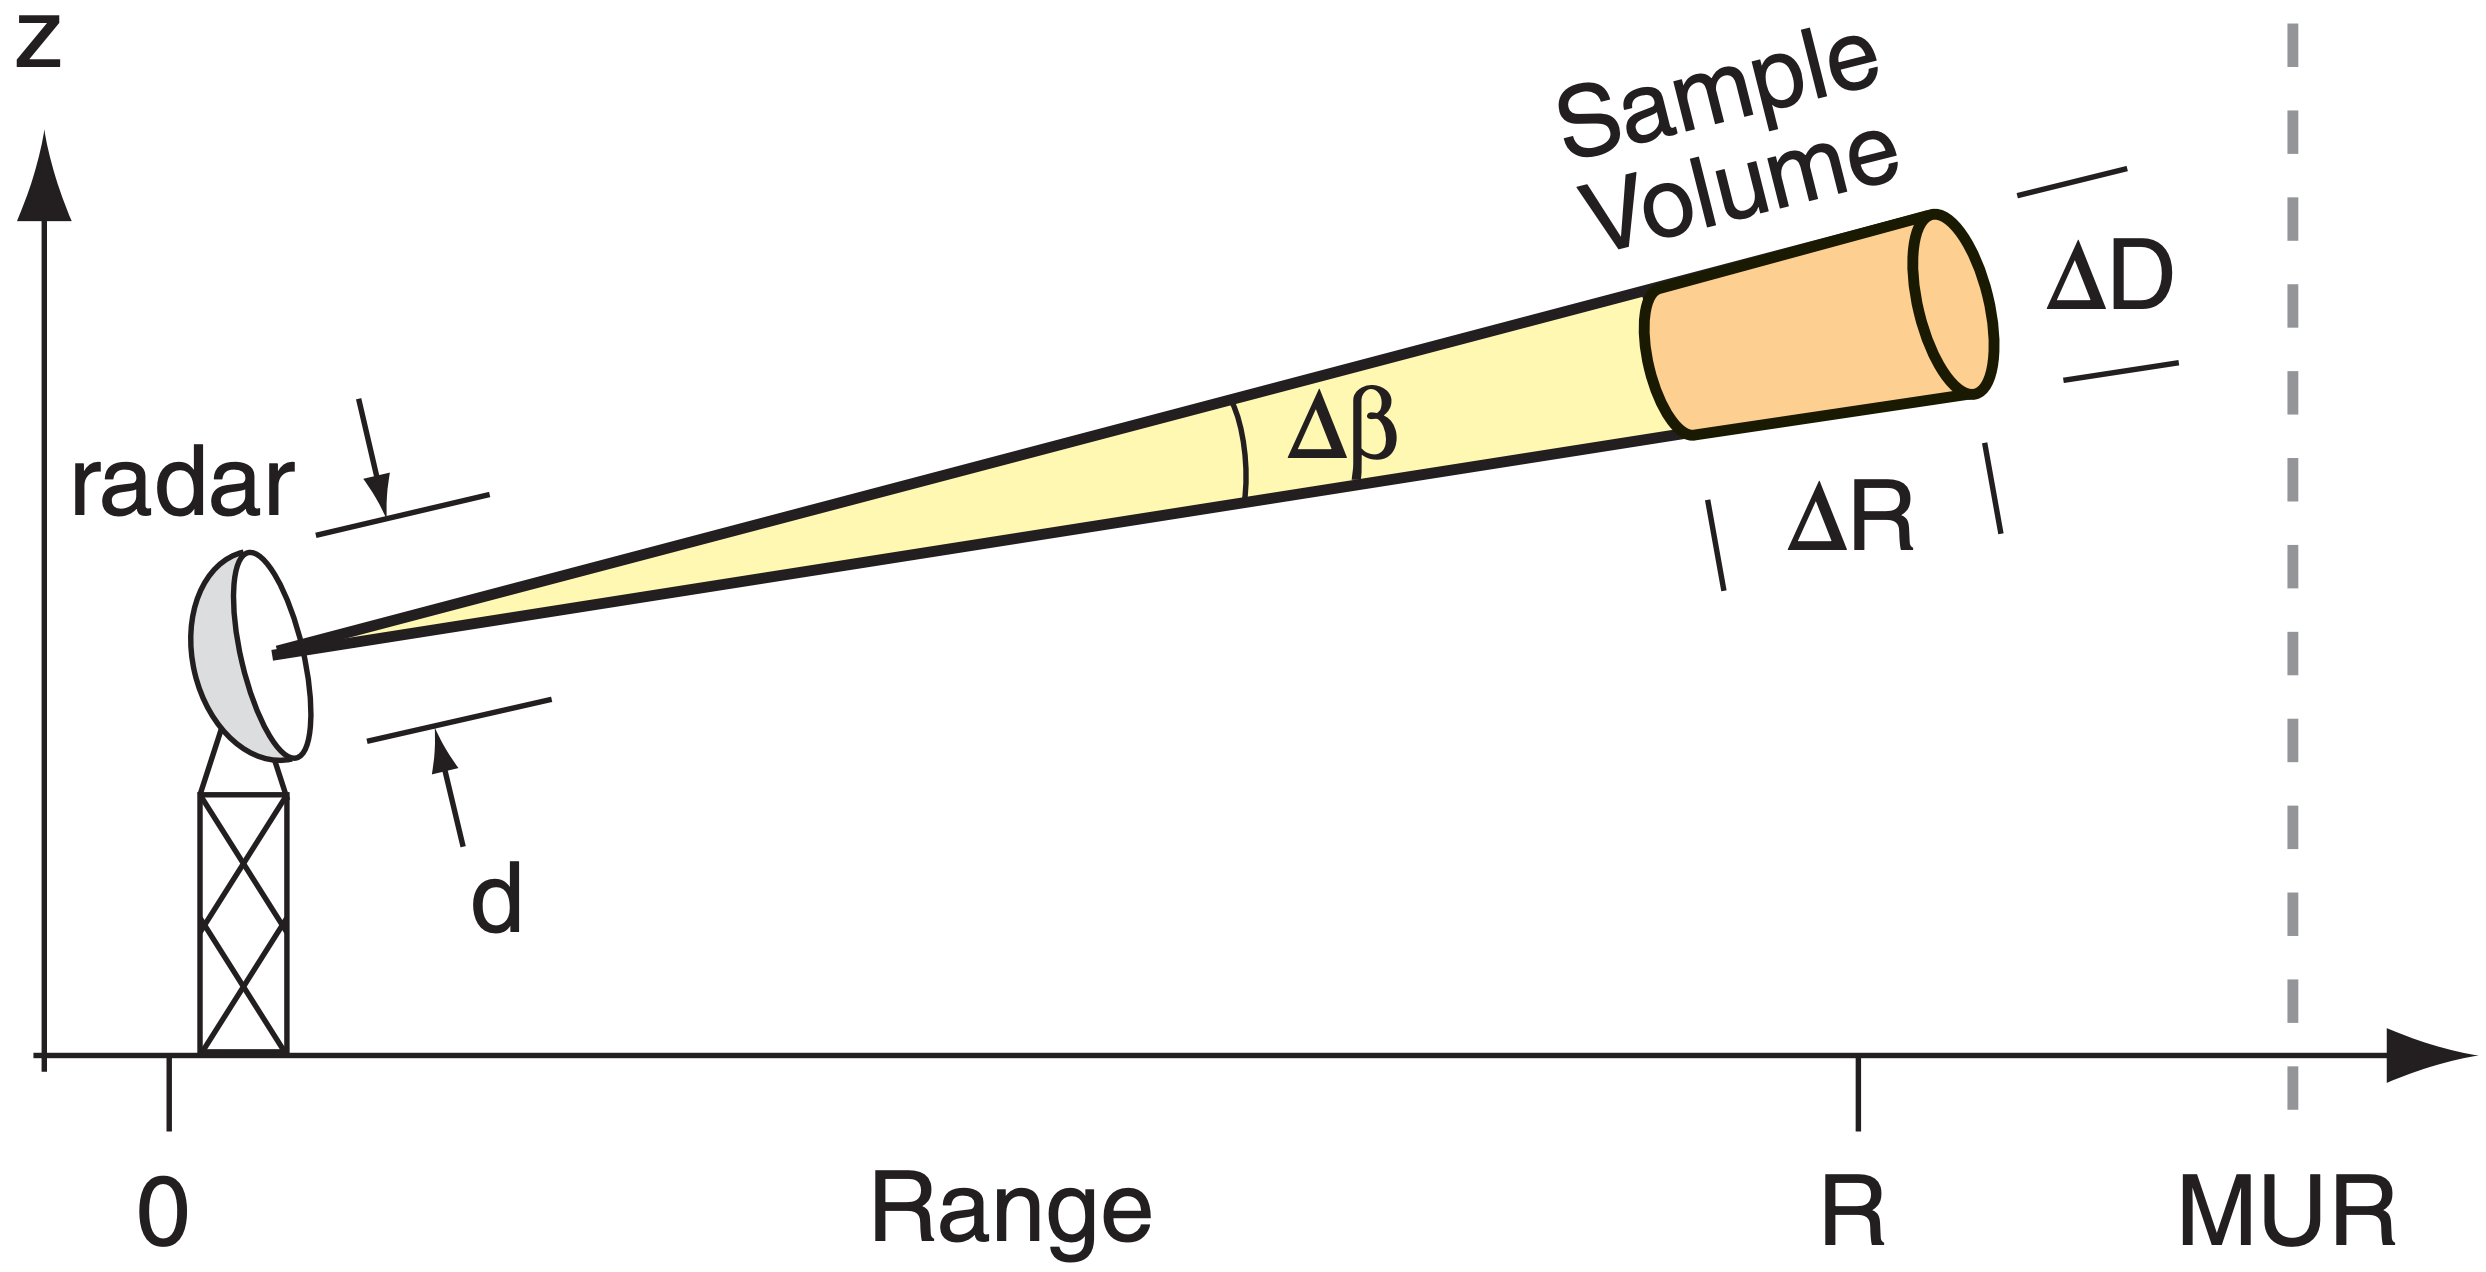
\includegraphics[width=0.8\linewidth]{Images/radar_concept.png}
    \vspace{1cm}
    \caption{A typical meteorological radar \cite{2022Weather}}
    \label{fig:radar}
\end{figure}

\subsection{Basic terminologies}

\subsubsection*{Weather Radar}
% \footnote{Tên tiếng Việt của các thuật ngữ sẽ được căn cứ dựa trên TCVN
% 12636-12 : 2021 \cite{vn_meteor_standard}} Radar thời tiết là một loại cảm
% biến có khả năng phát sóng vô tuyến (bước sóng trong phạm vi từ 250 - 1000 kW)
% \cite{2022Weather}. Để gia tăng cường độ sóng, một chảo antent (attenna dish)
% hình parabol được sử dụng nhằm hội tụ bước sóng. Radar có thể nâng và hạ (tuỳ
% theo yêu cầu) để thu nhập thông tin tại các vị trí chỉ định trong không gian 3
% chiều.

Weather radar, short for weather surveillance radar, is a type of radar system
used to detect and monitor precipitation, as well as other atmospheric phenomena
such as the movement of severe weather systems. It plays a crucial role in
meteorology and helps meteorologists track and forecast weather conditions.
Normally, weather radars are programmed to scan in an azimuth of $360^o$. For
every round, the radar will scan at a different altitude. It usually takes about
four to ten minutes for the radar to complete a full scan.

For PPI representation, the radar will scan the entire azimuth, but only at a
certain altitude. The final result would be similar to a map on a flat surface.
For RHI, in contrast, the radar retains the azimuth but increases in altitude.
The collected result gives viewers more details about the height and sizes of a
meteorologist event.

\begin{figure}[H]
    \centering
    \begin{subfigure}{\textwidth}
        \centering
        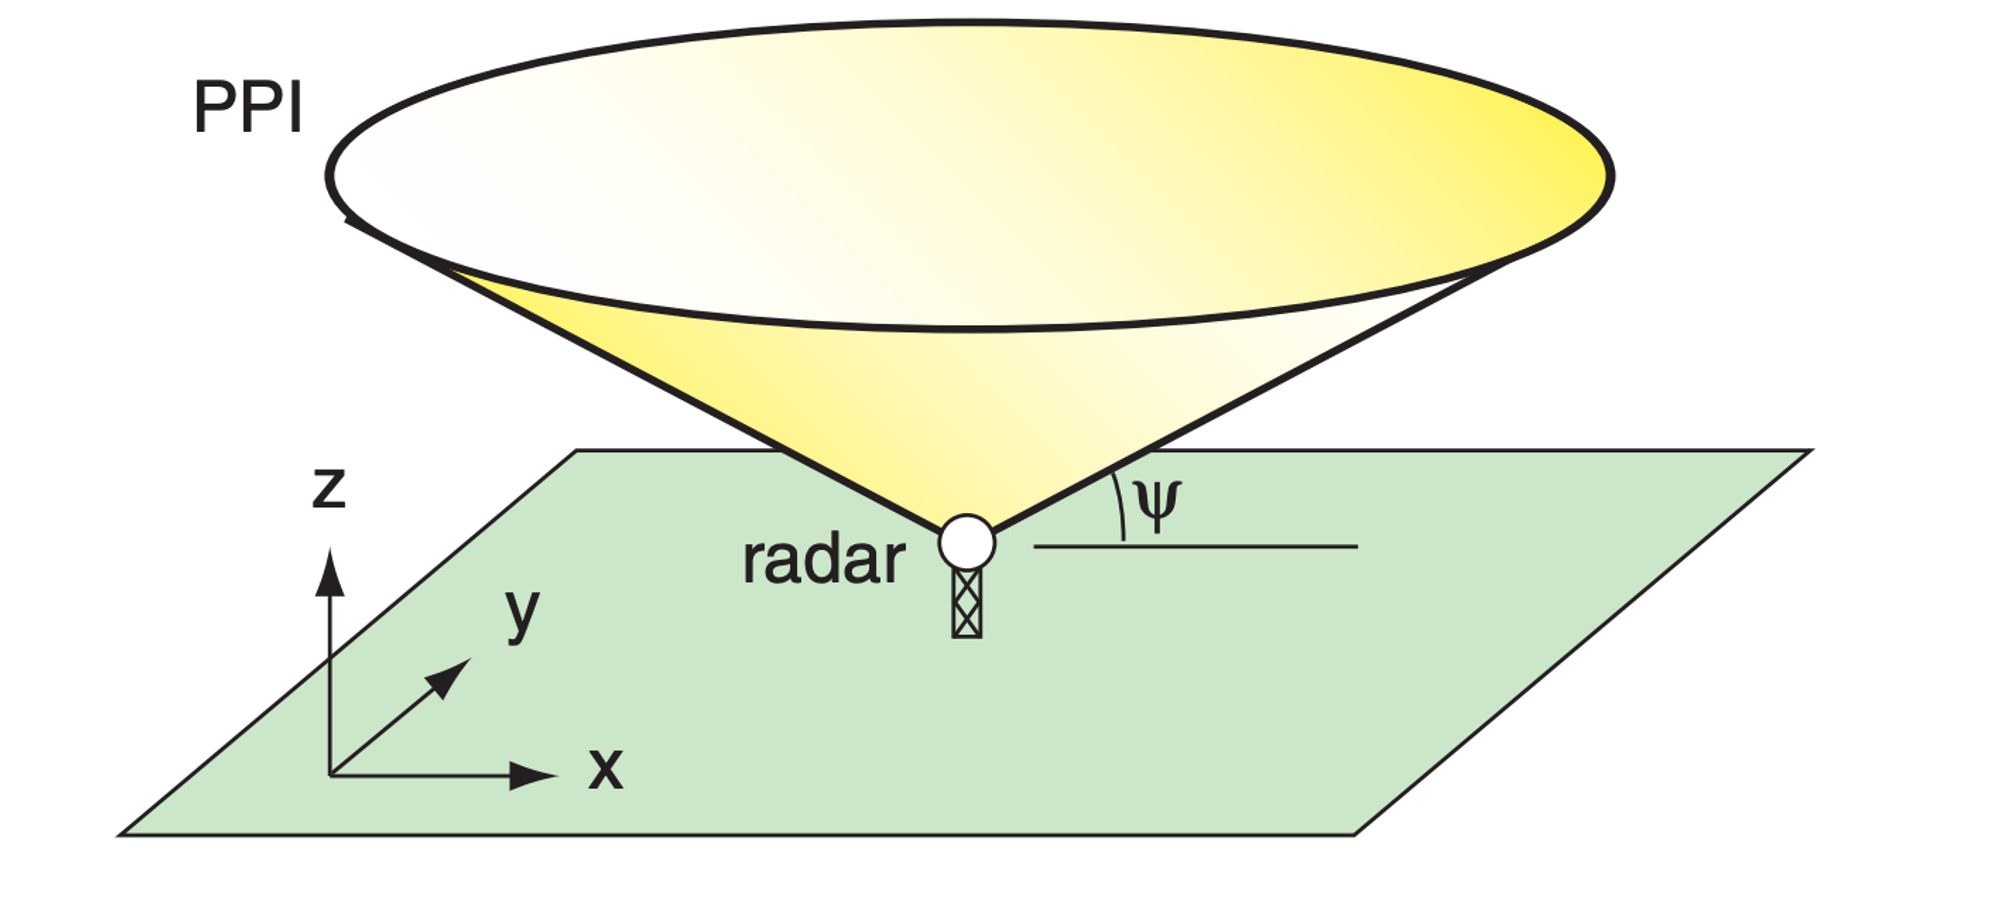
\includegraphics[width=0.85\textwidth]{Images/2.1-ppi.png}
        \caption{Plan-Position Indicator - PPI - \cite{2022Weather}}
        \label{fig:ppi}
    \end{subfigure}

    \begin{subfigure}{\textwidth}
        \centering
        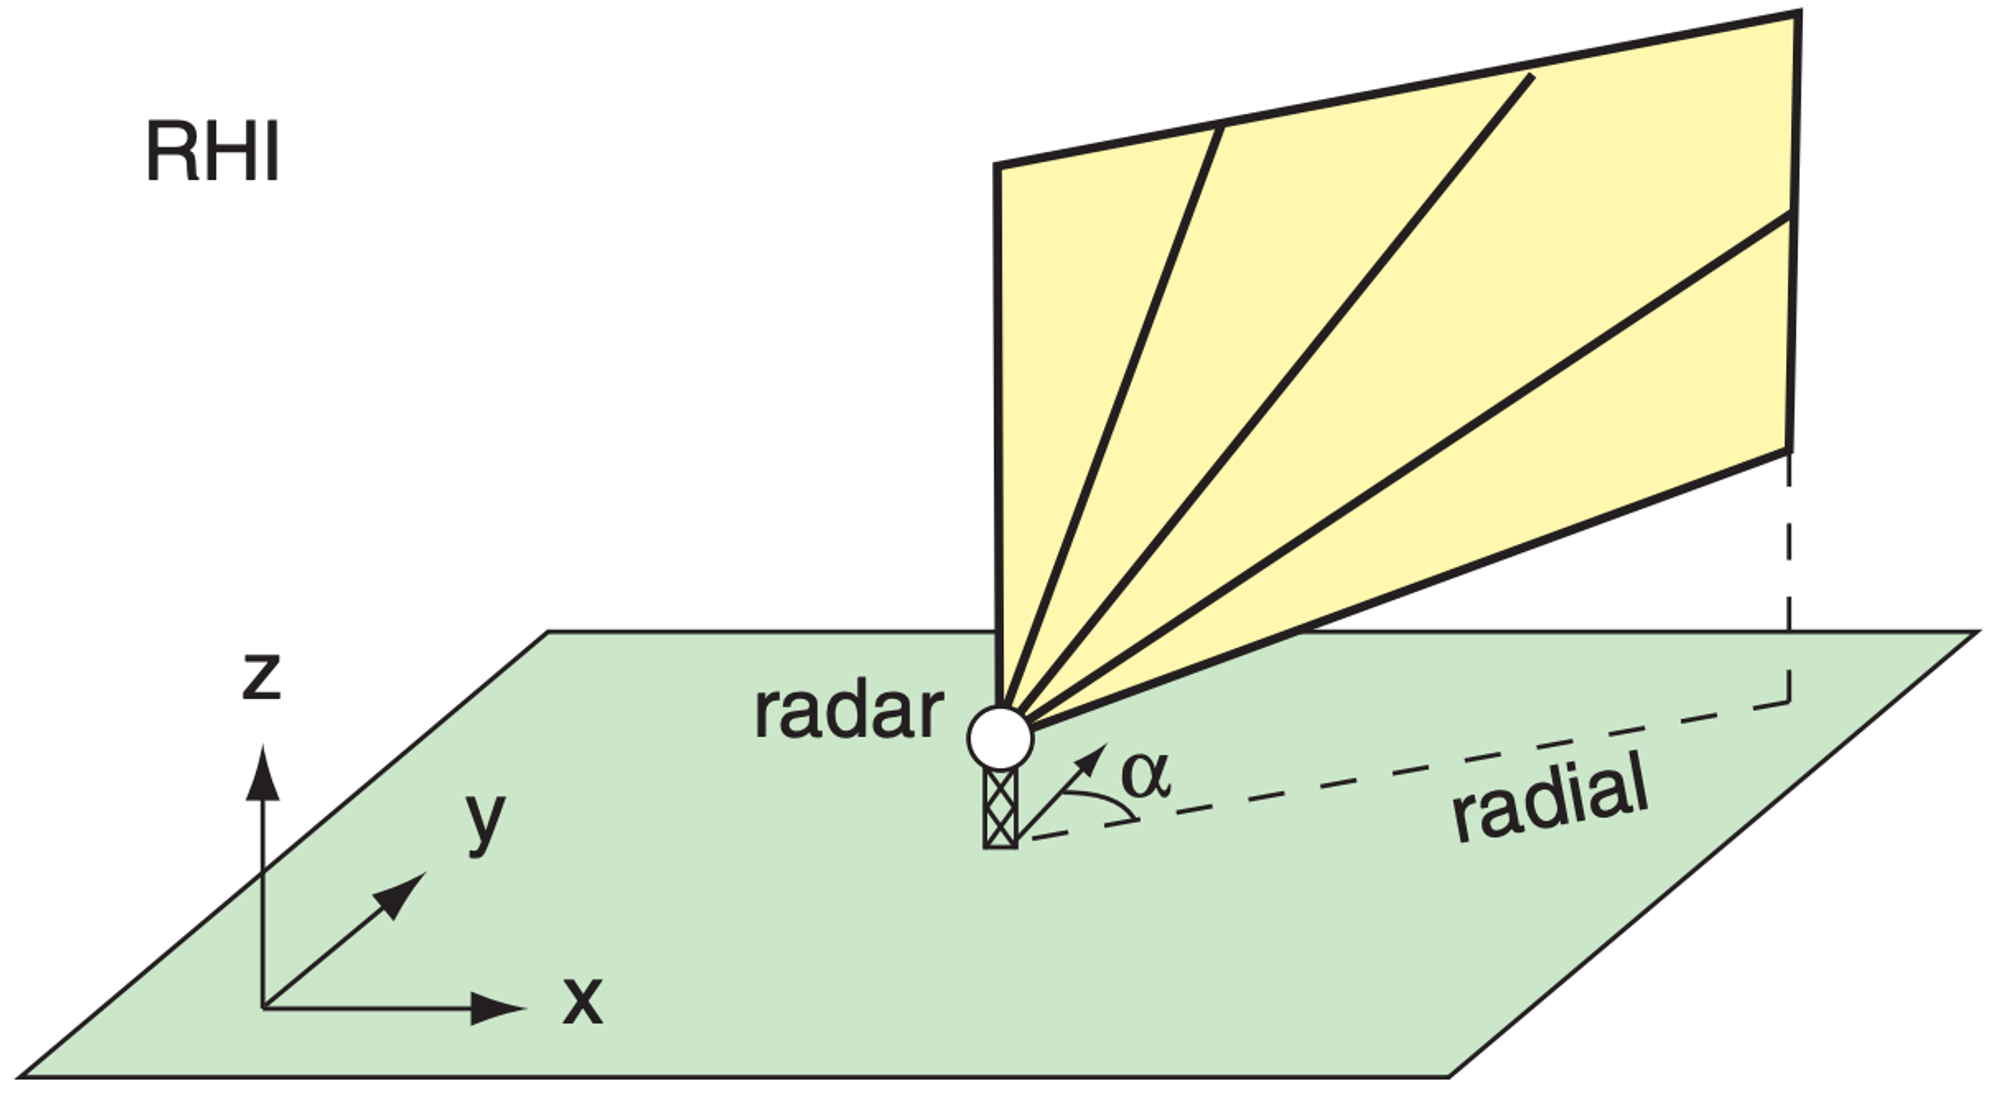
\includegraphics[width=0.85\textwidth]{Images/2.1-rhi.png}
        \caption{Range Height Indicator - \cite{2022Weather}}
        \label{fig:rhi}
    \end{subfigure}

\end{figure}



\begin{figure}[H]
    \centering
    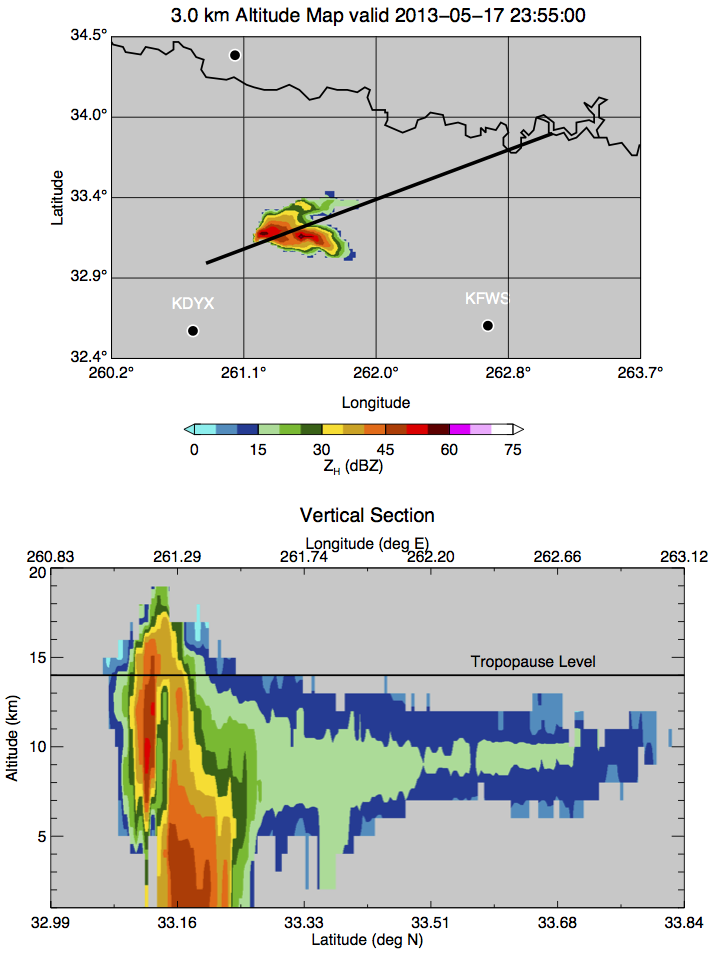
\includegraphics[width=\linewidth]{Images/2.1-ppi-and-rhi.png}
    \caption{Comparing the result between PPI and RHI -
    \cite{stackexchange-ppi-rhi}}
    \label{fig:ppi-and-rhi}
\end{figure}

\subsubsection*{Radar equation and Reflectivity}
At a certain point in time, weather radar will emit a short pulse of radio wave
($\Delta t = 0.5 - 10 \mu s$). Depending on the density of free molecules in the
air (water vapor, smoke, ...), the energy of this wavelength will be partially
absorbed. The wavelength intensity that the radar receives will be less than the
intensity of the original wave. This ratio is expressed through \textbf{The
radar equation} \cite{2022Weather}:

\[
    \left[ \frac{P_R}{P_T} \right]=\left[ b \right]\cdot\left[ \frac{|K|}{L_a} \right]^2\cdot\left[ \frac{R_1}{R} \right]^2\cdot\left[ \frac{Z}{Z_1} \right]
\]
\vspace{0.5cm}

Which, the variables of the equation include:
\begin{itemize}
    \item $|K|$ unitless:
          \begin{itemize}
              \item $|K|^2 \approx 0.93$ for droplets
              \item $|K|^2 \approx 0.208$ for ice crystal
          \end{itemize}
    \item $R (\text{km})$: distance from the radar to the target
    \item $R_1 = \sqrt{Z_1 \cdot c \cdot \Delta t / \lambda^2}$: ratio of
    distance
    \item $Z$: Radar\'s reflectivity
    \item $Z_1 = 1 \text{ mm}^6 \text{ m}^{-3}$: Radar's unit reflectivity
\end{itemize}

From the radar equation, we can derive the formula for reflectivity:
\vspace{0.5cm}
\[
    \text{dBZ} = 10\left[ \log\left( \frac{P_R}{P_T} \right) + 2 \log\left( \frac{R}{R_1} \right) - 2\log\left| \frac{K}{L_a} \right| - \log\left( b \right) \right]
\]

Meteorologists are usually interested in this number because it is proportional
to the amount of precipitation.

\begin{table}[H]
    \centering
    \begin{tabular}{|c|l|}
        \hline
        Value (dBZ) & Weather               \\
        \hline
        -28         & Haze                  \\
        -12         & Clear air             \\
        25 - 30     & Dry snow / light rain \\
        40 - 50     & Heavy rain            \\
        75          & Giant hail            \\
        \hline
    \end{tabular}
    \vspace{1em}
    \caption{ Relation between reflectivity and precipitation -
    \citet{2022Weather}}
\end{table}

\begin{figure}[H]
    \centering
    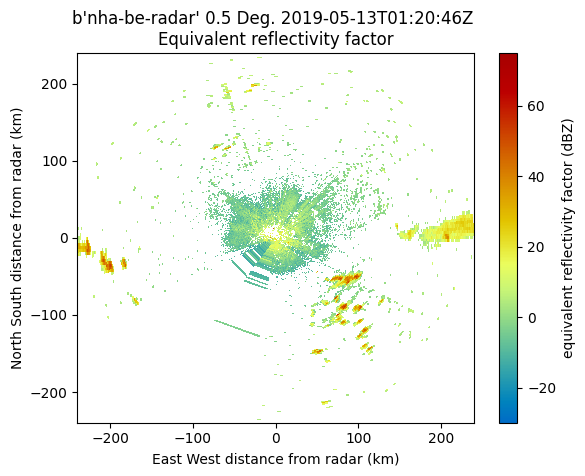
\includegraphics[width=0.75\textwidth]{Images/2.1-reflectivity_nhabe.png}
    \vspace{1em}
    \caption{Reflectivity from Nha Be radar}
    \label{fig:reflectivity-nhabe}
\end{figure}

\subsubsection*{Radial velocity}

\begin{figure}[H]
    \centering
    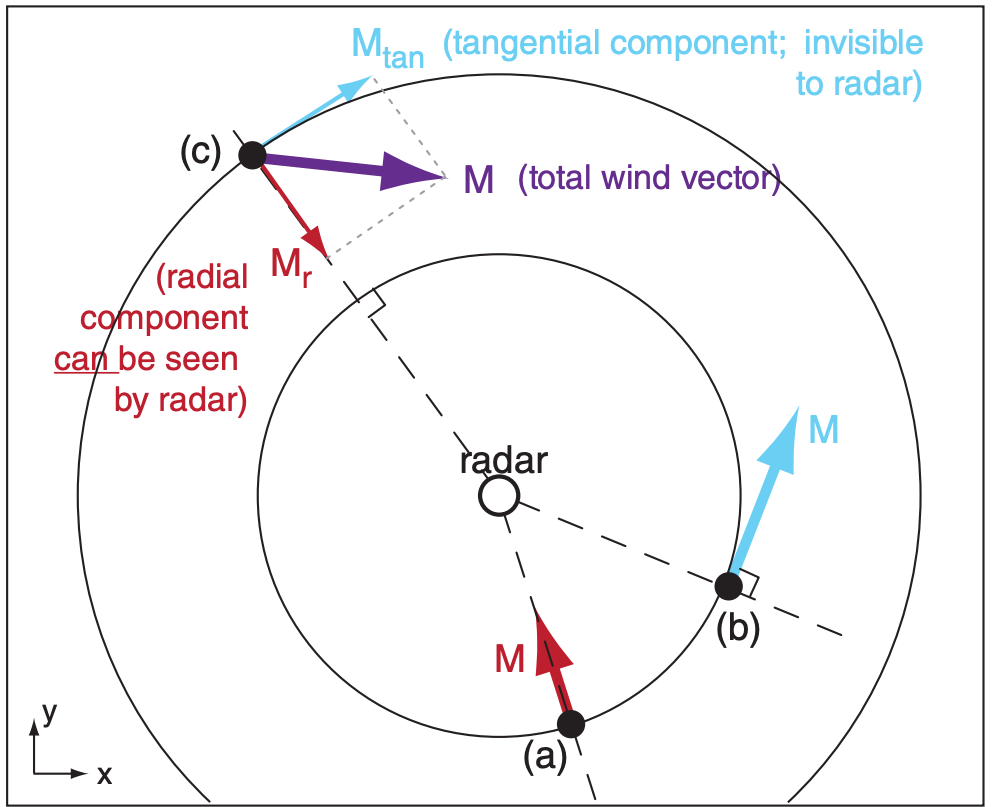
\includegraphics[width=.55\textwidth]{Images/2.1-radial-velocity.png}
    \vspace{2em}
    \caption{Illustration for the velocity situations that a Doppler radar can
    observe. (a) When the wind direction at point M coincides with the radius of
    the circle centered at the radar, the radar can determine the velocity at
    this point. (b) When the wind direction is tangent to the circle, the radar
    cannot determine the velocity. (c) Analyzing the wind direction at M into
    two perpendicular velocities, the radar can only determine the velocity
    vector along $M_r$.  - \citet{2022Weather}}
    \label{fig:radial-velocity}
\end{figure}

When the radio waves from these Doppler radars propagate to the molecules in the
air, the displacement of these particles causes a phase shift between the
transmitted and received signals. Radars rely on this information to calculate
the wind velocity at various points in space.

\subsection{Radar Products}



\subsubsection*{Echo Top Height (ETH)}

In radar meteorology, an echo top signifies the highest altitude at which
precipitation particles are detected. Essentially, it pinpoints the maximum
elevation angle where the intensity of precipitation, quantified by
reflectivity, surpasses a predetermined threshold. This information is crucial
for understanding the vertical extent of precipitation systems and their
potential impact.

The modified ETH algorithm, developed by Lakshmanan et al. (2013)
\cite{lakshmanan2013}, can be applied to a NEXRAD PPI volume scan through a
systematic approach. Initially, the maximum elevation angle, denoted by
$\theta_{b}$, where the reflectivity, $Z_{b}$, exceeds a predefined echo-top
reflectivity threshold, $Z_T$ (e.g., 0 dBZ, 18 dBZ), is located. If $\theta_{b}$
is not the highest elevation scan available in the volume, the reflectivity
value, $Z_{a}$, at the subsequent higher elevation angle, $\theta_{a}$, is
obtained. The echo-top height, $\theta_T$, is then calculated using the
following equation:

\[ \theta_T = \frac{(Z_T - Z_a)(\theta_b - \theta_a)}{Z_b - Z_a} + \theta_b \]

In cases where $\theta_{b}$ coincides with the highest elevation scan
accessible, $\theta_{T}$ is set to $\theta_{b} + \beta/2$, where $\beta$
represents the half-power beamwidth. This scenario typically occurs either far
from the radar, where higher elevation scans have shorter ranges compared to a
baseline "surveillance" scan, or very close to the radar, where the highest
elevation scan fails to capture the cloud's peak.

Under these circumstances, $\theta_{T}$ corresponds to the top of the beam
containing reflectivity greater than or equal to $Z_T$. Thus, the traditional
echo-top computation is adopted when no data exists from higher elevation scans.

The mathematical formulation of this can be expressed as:

\[ 
\theta_T = \begin{cases} 
\frac{(Z_T - Z_a)(\theta_b - \theta_a)}{Z_b - Z_a} + \theta_b & \text{if } \theta_b \text{ is not the highest elevation scan} \\
\theta_b + \frac{\beta}{2} & \text{if } \theta_b \text{ is the highest elevation scan} 
\end{cases}
\]

This equation incorporates a conditional statement to account for the two
scenarios based on the availability of data from higher elevation scans.

\subsubsection*{Plan Position Indicator (PPI)}

The Plan Position Indicator (PPI) is the most common type of radar display. It
shows a horizontal slice of radar data at a fixed elevation angle. The PPI scan
provides the intensity of returned echoes from targets such as raindrops,
snowflakes, or hail. The radar emits pulses at a specific elevation angle
$\theta$ and records the returned signal. The range $r$ to the target is
calculated based on the time delay of the returned signal:

\[
r = \frac{c \Delta t}{2}
\]

where $c$ is the speed of light and $\Delta t$ is the time delay. The PPI
displays this data in polar coordinates, with the azimuth angle $\phi$ and range
$r$ as the primary variables. This display helps in determining the structure of
storms, the intensity of precipitation, and features such as fronts and squall
lines.

\subsubsection*{Constant Altitude Plan Position Indicator (CAPPI)}

The Constant Altitude Plan Position Indicator (CAPPI) provides radar
reflectivity data at a constant altitude above the radar site. This product is
created by interpolating data from multiple elevation scans to represent
reflectivity at a specified altitude $h$. The interpolation uses the
reflectivity values $Z(\theta_i, r_i)$ from different elevation angles
$\theta_i$ and ranges $r_i$, and projects them to the desired constant altitude:

\[
Z_{CAPPI}(h) = f(Z(\theta_1, r_1), Z(\theta_2, r_2), \ldots, Z(\theta_n, r_n))
\]

where $f$ denotes the interpolation function. CAPPI overcomes limitations posed
by the Earth's curvature and terrain obstructions, providing a clearer picture
of precipitation distribution at a constant altitude, aiding in tracking and
analyzing the horizontal spread and intensity of precipitation within storms.

\subsubsection*{Maximum Echo Height (HMAX)}

Maximum Echo Height (HMAX) displays the maximum altitude at which significant
radar echoes are detected within each radar sweep area. HMAX is calculated by
determining the highest elevation angle $\theta_i$ at which the reflectivity
$Z_i$ exceeds a predefined threshold $Z_T$. The height $h_i$ corresponding to
$\theta_i$ and range $r_i$ is given by:

\[
h_i = r_i \sin(\theta_i) + H_r
\]

where $H_r$ is the radar height above sea level. The maximum height $H_{max}$ is
then:

\[
H_{max} = \max(h_i \mid Z_i \geq Z_T)
\]

HMAX helps in understanding the vertical development of thunderstorms and is
used to gauge storm intensity and potential severe weather occurrences.

\subsubsection*{Composite Maximum Reflectivity (CMAX)}

Composite Maximum Reflectivity (CMAX) provides a top-down view of the highest
reflectivity measured at any altitude within the volume of a radar scan. CMAX is
generated by compiling the maximum reflectivities $Z_{max}$ from all elevation
scans into a single image. For each horizontal grid point $(x, y)$, CMAX is
given by:

\[
Z_{CMAX}(x, y) = \max(Z(\theta_i, r_i) \mid (x_i, y_i) \in (x, y))
\]

where $(x_i, y_i)$ are the horizontal coordinates corresponding to the radar
coordinates $(\theta_i, r_i)$. CMAX is valuable for identifying the strongest
areas of storms across multiple altitudes, highlighting potential regions of
severe weather. It allows forecasters to quickly assess the overall intensity of
precipitation and identify the most significant storm cells over a large area.


\section{Common Data format in meteorology}
\subsection{SIGMET data format - raw format (Vaisala)}
\label{sigmet}
Vaisala, a Finnish company renowned for its expertise in environmental and
meteorological instrumentation, has developed the RAW format, also known as
SIGMET \cite{lrose_RadxConvert}, as a specialized storage format for organizing
data output from its radar devices. This format represents a meticulously
designed system tailored to efficiently manage the voluminous data generated by
radar scanning sessions.

Distinctive features characterize the architecture of the RAW format. Notably,
the file content is partitioned into discrete blocks, each precisely sized at
6144 bytes. This particular sizing aligns with historical conventions rooted in
the main storage capacities of older tape devices, reflecting a pragmatic
approach to data organization and storage optimization. Furthermore, the RAW
format typically consolidates data from multiple radar scanning sessions within
a single file, fostering data aggregation and accessibility.

Within each block of the RAW format, data records are meticulously structured,
ensuring efficient utilization of storage space. In instances where space within
a block remains unoccupied after accommodating data records, padding with
additional zeros is employed, maintaining structural integrity and facilitating
streamlined data retrieval processes.

The adoption of the RAW format confers several notable advantages, as elucidated
by empirical analyses and industry insights \cite{raw_product_format_vaisala}. Firstly, the format
demonstrates inherent compatibility with a diverse array of tape types, a legacy
consideration owing to the historical prevalence of tape-based storage systems.
Despite the evolution of storage technologies, tapes persist as cost-effective
alternatives, underscoring the ongoing relevance and practicality of the RAW
format in contemporary data management contexts. Moreover, the block-oriented
architecture of the RAW format facilitates robust error recovery mechanisms at
the storage system level, enhancing data reliability and resilience against
potential hardware failures.

Despite its merits, concerns persist regarding the alignment of the storage
structure delineated by the RAW format with the corresponding mappings on hard
drives and tape devices. Addressing these concerns necessitates meticulous
attention to compatibility and interoperability considerations, ensuring
seamless data interchangeability across heterogeneous storage environments.

In essence, the RAW format epitomizes Vaisala's commitment to innovation and
excellence in the domain of environmental instrumentation. Its tailored design
and inherent advantages render it a formidable tool for efficiently managing and
organizing radar data, thereby empowering researchers and practitioners in
meteorology and related fields with robust data management capabilities.

\subsection{NETCDF data format - Network Common Data Form}

The Network Common Data Form (NetCDF) \cite{netcdf} represents a pivotal file
format meticulously engineered for the purpose of accommodating multidimensional
scientific data. Embedded within the framework of the NetCDF library system are
a variety of binary formats, each strategically contributing to the overarching
flexibility and scalability of data management within scientific domains. These
formats, which have evolved over iterations of the NetCDF library system, are
emblematic of its adaptability to diverse data requirements and computational
environments.

\begin{figure}[H]
    \centering
    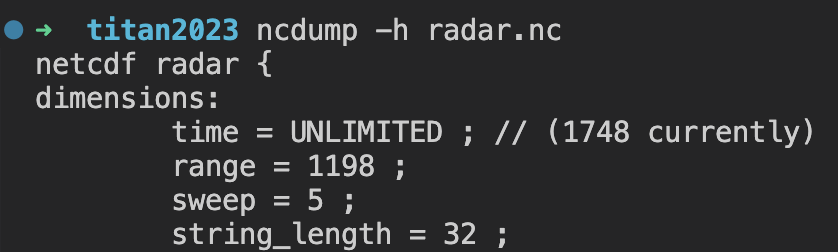
\includegraphics[width=1\linewidth]{Images/ncdump.png}
    \vspace{1em}
    \caption{Radar information in NETCDF format. The total dimensions of the dataset are 2975, grouped into 4 distinct labels.}
    \label{fig:enter-label}
\end{figure}


Foremost among these formats is the Classic Format, which has been a mainstay
since the inception of the NetCDF library and continues to serve as the default
option for file creation. Over time, subsequent releases of the NetCDF library
system have introduced additional formats, each with distinct features tailored
to specific demands. The 64-bit Offset Format, for instance, emerged with
version 3.6.0, addressing the need for expanded variable and file sizes beyond
the limitations of its predecessors.

In a similar vein, the integration of the netCDF-4/HDF5 Format with the release
of version 4.0 represents a milestone in the evolution of the NetCDF ecosystem.
By harnessing the capabilities of the Hierarchical Data Format version 5 (HDF5),
this format bridges the gap between the NetCDF and HDF5 data models, offering
users enhanced capabilities such as support for unlimited dimensions and
substantially larger file sizes. Furthermore, the incorporation of the HDF4 SD
Format and the CDF5 Format underscores the NetCDF ecosystem's commitment to
interoperability and compatibility with parallel processing frameworks.

Central to the design philosophy of NetCDF formats is the concept of
self-description, wherein comprehensive metadata, including attribute name/value
pairs and data array structures, are encapsulated within the file header. This
design not only fosters platform independence but also facilitates seamless data
exchange and interoperability across diverse computational environments.

To illustrate the versatility and efficacy of the NetCDF format, consider a
practical scenario involving the storage of meteorological parameters, including
temperature, humidity, pressure, wind speed, and direction, within NetCDF files.
This exemplifies the format's capacity to accommodate complex, multidimensional
datasets characteristic of scientific research domains, thereby empowering
researchers with a robust and flexible tool for data management and analysis.


Furthermore, it is noteworthy that NetCDF Classic and 64-bit Offset Formats have
garnered international recognition as standards endorsed by the Open Geospatial
Consortium (OGC), underscoring their role as reliable and interoperable
solutions for geospatial data management \cite{ogcnetcdf}. This validation not
only speaks to the robustness and reliability of the NetCDF format but also
underscores its global scalability and compatibility with established standards
and practices in the scientific community.
\section{Related technologies}
\subsection{Apache Airflow™}
Apache Airflow™ stands as an open-source platform designed to manage data flow
within systems associated with data. In the face of the escalating challenge of
data pipeline management, Airflow emerges as a comprehensive solution,
automating and optimizing data-related workflows effectively \cite{airflow}.

Airflow not only aids in defining and managing the start and end times of each
data pipeline but also provides precise and detailed monitoring of the results
of each task. This becomes particularly crucial when ensuring the integrity and
reliability of the processed data.

With the ability to discern complex relationships between tasks through the
Directed Acyclic Graph (DAG) model, Airflow empowers administrators with tighter
control and flexibility in handling workflow processes. Its robust integration
with logging systems facilitates detailed activity tracking, assisting in issue
resolution and ensuring that every process aligns with expectations.

Simultaneously, the scheduling flexibility makes Airflow an excellent tool for
time and resource management. Its strong integration with various data sources
and extensibility through plugins allows Airflow to meet diverse needs in data
processing and task automation.

Apache Airflow not only delivers robust performance but also brings flexibility
and optimal technical features to data processing workflows. With its time
management capabilities, powerful logging integration, scheduling flexibility,
and scalability, Airflow stands as the top choice for enhancing performance and
control in data processing workflows.

\subsection{Kubernetes}
Kubernetes, an open-source system for managing and deploying highly flexible
applications in cloud and data center environments, has evolved into one of the
most widely adopted tools in the field of Information Technology \cite{k8s-doc}.
Originally developed by Google and later transferred to the Cloud Native
Computing Foundation (CNCF), Kubernetes aims to automate the deployment,
scaling, and management of containerized applications, alleviating the burden on
developers and system administrators. The platform offers a unified foundation
for deploying, scaling, and managing containerized applications across multiple
servers.

Kubernetes operates based on key concepts such as Pods, Services, ReplicaSets,
and various other abstractions, creating a flexible environment for application
deployment and management. This fosters an environment where developers can
easily build applications, and system administrators can efficiently maintain
them.

Beyond supporting traditional deployment models, Kubernetes paves the way for
innovative strategies like Continuous Deployment (CD) and Microservices. With
the ability to automate many aspects of the development and deployment process,
Kubernetes plays a crucial role in constructing and sustaining complex,
flexible, and scalable systems.

\subsubsection*{Kubernetes Components}
Introducing essential concepts for managing and deploying applications,
Kubernetes provides an effective and flexible environment. The main components
of Kubernetes include Pod, ReplicaSet, Deployment, and Service.

\begin{figure}[H]
    \centering
    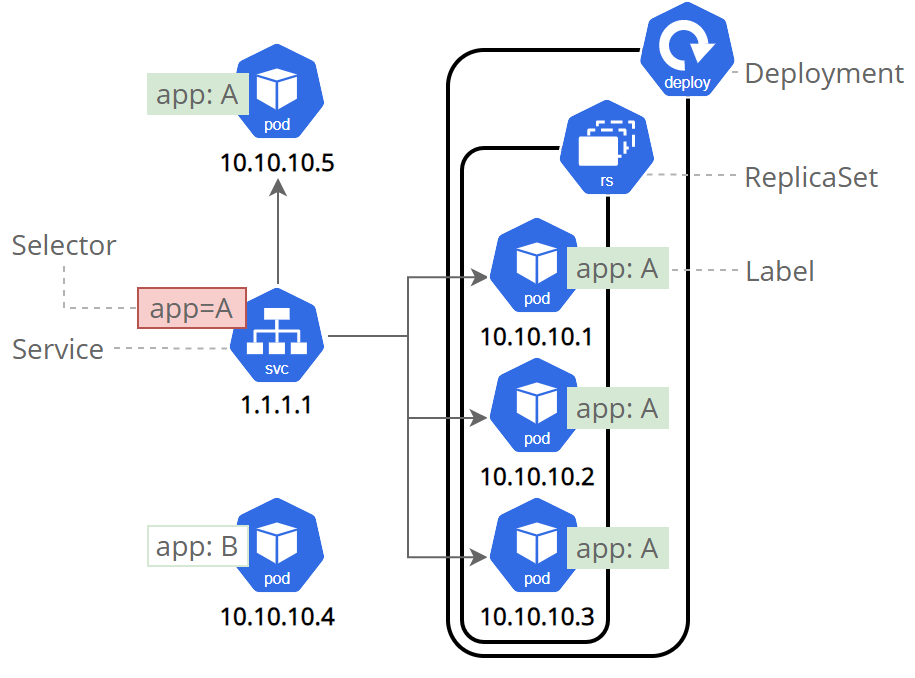
\includegraphics[width=0.75\linewidth]{Images/3.4-k8s-comps.png}
    \caption{Overview of Kubernetes Components - Kubernetes}
    \label{fig:k8s-comps}
\end{figure}

In Kubernetes, a \textbf{Pod} serves as the fundamental unit, representing a
collection of containers that share a common workspace. Within the same Pod,
containers collaborate by sharing network and storage resources, fostering
interaction and enabling the construction of intricate applications.

The \textbf{ReplicaSet}, a crucial resource in Kubernetes, ensures a designated
number of Pods operate in a specified manner. In the event of a Pod failure or
shutdown, the ReplicaSet automatically initiates the creation of a new Pod to
replace it. This mechanism ensures the application's stable state by
guaranteeing a defined number of Pods are consistently operational.

For managing the deployment and updating processes of applications,
\textbf{Deployment} is a key component in Kubernetes. It articulates the desired
state of the application and orchestrates the updating of the ReplicaSet to
achieve that state. Deployment provides versatile management capabilities,
facilitating the deployment of new versions, rollbacks, and updates without
disrupting the service.

The \textbf{Service} resource in Kubernetes furnishes an HTTP port to Pods,
generating a unique IP address and DNS name for a cluster of Pods. This enables
seamless communication among applications within the cluster and with external
environments. Service effectively simplifies the intricacies of handling
multiple Pods and IP addresses, offering a straightforward means of accessing
services within the Kubernetes environment.

Typically, large-scale systems leverage Kubernetes in their software development
and deployment processes. This adoption brings several advantages, including
efficient resource management and self-recovery capabilities. Kubernetes
optimizes resource utilization, ensuring optimal performance and reducing waste.
Additionally, it automatically addresses issues during operations, enhancing
high availability.

However, the technology is not without its challenges, including a steep
learning curve for beginners. Mastery of diverse knowledge areas such as
computer networking and containerization is necessary. Moreover, deploying and
maintaining Kubernetes demands significant resources, both in terms of personnel
and hardware, particularly for smaller organizations.

\subsubsection*{High Availability in Kubernetes}
High Availability is a crucial factor in the success of any system. In
Kubernetes, High Availability is achieved through the combination of several
features, including self-healing, load balancing, and auto-scaling.

First, Kubernetes uses \textbf{Deployment}, a type of \textbf{Controller} for
managing replicas. Through Deployment, we can easily perform horizontal scaling,
which is the process of increasing the number of replicas of a Pod. This
mechanism ensures that the application can handle numerous requests without
compromising performance. Moreover, in case of a Pod failure, a Deployment makes
sure that a new Pod is created to replace it, ensuring the amounts of predefined
replicas is always maintained.

At network layers, Kubernetes uses \textbf{Service} for communication between
various components within or outside the cluster. Instead of directly accessing
Pods, other components can access Services, which will redirect the request to
the appropriate Pod. When Pods are replaced, the Service will automatically
update the routing rules to ensure the request is sent to the correct Pod.
Outside the cluster, Kubernetes also uses \textbf{Ingress} to manage external
access to Services. Instead of specifying the direct node IP address, Clients
can abstract it by using only the URL or hostname.

Finally, at the storage level, Kubernetes provides Persistent Volumes. By doing
so, applications can be agnostic to the underlying storage infrastructure. This
allows for easier management and scaling of storage resources. Not only that,
depending on the provided \textbf{Storage Class}, Kubernetes makes sure that the
data is replicated to multiple nodes, ensuring data availability in case of node
failure.

To summarize, Kubernetes provides a robust set of features to ensure High
Availability. By leveraging these features, we can build a highly available
system that can scale with our load, while also being resilient to failures.

\subsection{LROSE}
LROSE (Lidar Radar Open Software Environment) is a project supported by the
National Science Foundation (NSF) with the goal of developing common software
for the Lidar, Radar, and Profiler community. The project operates based on the
principles of collaboration and open source. The core software package of LROSE
is a collaborative effort between Colorado State University (CSU) and the Earth
Observing Laboratory (EOL) at the National Center for Atmospheric Research
(NCAR) \cite{lrose}.

Originating from the need for a unified software environment for processing
Lidar and Radar data in atmospheric science research \cite{lrose}, the project
addresses complexities related to integrating data from various observation
platforms, including Lidar, Radar, and Profiler. These components are designed
to meet the specific needs of meteorologists and researchers working with remote
sensor data.

LROSE is widely used in meteorological research, including studies related to
cloud and precipitation processes, boundary layer dynamics, and other
meteorological phenomena. The software supports the analysis of observation data
collected from ground-based tools such as Lidar and Radar. LROSE seamlessly
integrates with a variety of model and atmospheric analysis tools to optimize
its capabilities. Researchers often integrate LROSE into numerical weather
prediction models as well as other data assimilation techniques, creating a
flexible and powerful system.

\begin{figure}[H]
    \centering
    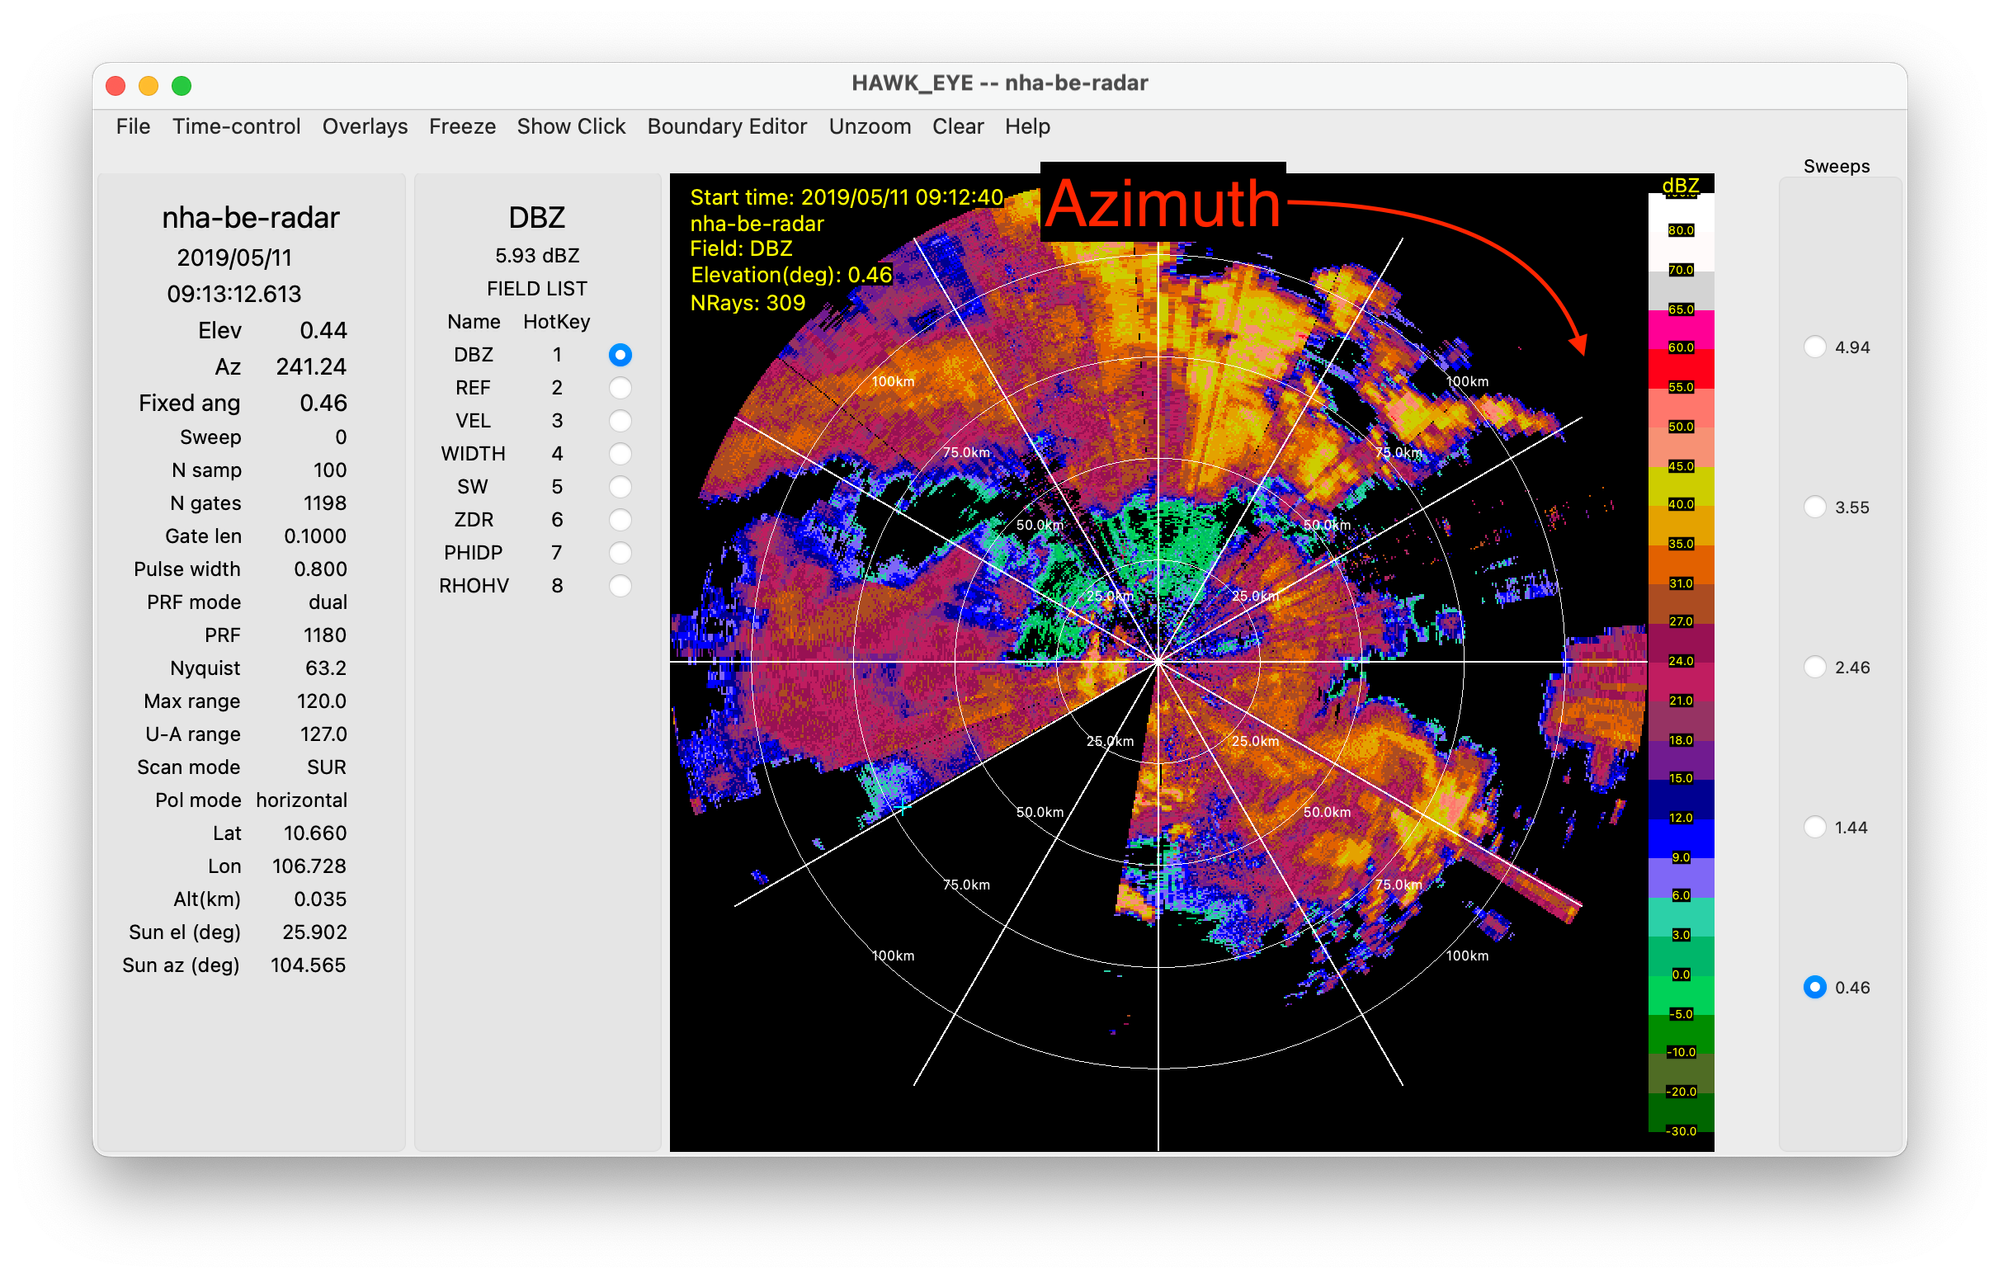
\includegraphics[width=0.8\linewidth]{Images/3.5-hawk-eye.png}
    \caption{Hawk Eye, Lidar and Radar visualization tool of LROSE}
    \label{fig:hawk-eye}
\end{figure}

The project actively encourages participation from a large scientific community,
promoting the exchange of ideas, algorithms, and improvements for the software.
Regular updates and contributions from users contribute to the continuous
development and refinement of LROSE.

% =================================================================================
% Py-ART
% =================================================================================

\subsection{Py-ART}
In the realm of meteorology, weather radar plays a crucial role in understanding
and forecasting precipitation, cloud cover, and other atmospheric phenomena.
Extracting meaningful information from this data requires specialized tools and
techniques. Py-ART (the Python ARM Radar Toolkit) is an open-source Python
library designed specifically for working with weather radar data.

Developed by the Atmospheric Radiation Measurement (ARM) Climate Research
Facility, Py-ART offers a comprehensive suite of algorithms and utilities for
researchers and atmospheric scientists. However, its user-friendly design and
extensive functionalities make it valuable for anyone working with weather radar
data, from meteorologists to students.

\subsubsection*{Core functionalities}
Py-ART transcends its role as a simple data repository. It empowers users with a
comprehensive suite of functionalities, transforming raw weather radar data into
meaningful insights.  At its core, Py-ART offers a robust toolbox for data
manipulation, analysis, and visualization, catering to the diverse needs of
meteorologists, researchers, and anyone working with weather radar information.

The journey begins with seamless data access. Py-ART supports a wide range of
file formats commonly used in atmospheric research. This versatility allows
users to import data from various sources, eliminating compatibility hurdles and
streamlining the workflow. Once the data is loaded, Py-ART's processing
capabilities come into play. Real-world radar measurements are not without
imperfections. Signal attenuation, caused by factors like distance and
intervening obstacles, weakens the returning signal. Py-ART provides algorithms
to correct for this attenuation, ensuring the accuracy of the retrieved
information. Furthermore, raw radar data often contains noise – unwanted
electrical disturbances that can distort the signal. Py-ART offers a variety of
filtering techniques to remove this noise, resulting in a cleaner and more
reliable dataset. Calibration, a crucial step in ensuring data integrity, is
also made possible by Py-ART. By applying calibration techniques, users can
account for systematic biases inherent in the radar system, leading to more
precise measurements.

Once the data is cleaned and processed, Py-ART shines in its ability to
visualize and analyze this information. It seamlessly integrates with popular
scientific Python libraries like Matplotlib. This powerful combination allows
users to create informative and visually compelling representations of the data.
Imagine generating high-resolution reflectivity maps that paint a vivid picture
of precipitation intensity across a region. Py-ART facilitates this by
converting reflectivity data into maps, allowing for easy identification of
areas with heavy rain or snowfall.  Beyond maps, Py-ART enables the creation of
vertical profiles, which depict how reflectivity and other parameters vary with
altitude. This provides a detailed understanding of the vertical structure of
storms and precipitation events. Analyzing these visualizations in conjunction
with environmental data, which Py-ART can also incorporate, allows researchers
to delve deeper into the atmospheric processes at play.

Py-ART's functionalities extend beyond basic visualization. It offers advanced
analysis tools for tasks like feature detection and storm tracking. Imagine
automatically identifying and tracking the movement of severe weather features
like hailstorms or tornadoes within radar data. Py-ART's algorithms can
accomplish this, providing crucial information for issuing timely weather
warnings and protecting lives.  Perhaps the most impactful functionality lies in
quantitative precipitation estimation (QPE). By analyzing radar data and
incorporating environmental factors, Py-ART can estimate the amount of
precipitation that has fallen over a specific area. This information is
invaluable for flood forecasting, water resource management, and understanding
overall precipitation patterns.

\subsubsection*{Benefits}
Py-ART offers a range of benefits for working with weather radar data, making it
a compelling choice for meteorologists and atmospheric scientists alike.
Firstly, Py-ART is open-source and freely available, allowing anyone to access,
download, and modify its code. This fosters collaboration and innovation within
the atmospheric science community, as researchers can contribute improvements
and share their work with others.

Additionally, Py-ART boasts cross-platform compatibility, functioning seamlessly
on various operating systems including Windows, macOS, and Linux. This ensures
wider accessibility and flexibility for users across different computing
environments.

The modular design of Py-ART is another key advantage, allowing users to
leverage specific functionalities they need for their radar data processing
tasks. This modular approach enhances efficiency and adaptability, as users can
tailor their workflow to suit their requirements.

Moreover, Py-ART provides extensive documentation and a rich collection of
examples, which serve to ease the learning curve for new users. The availability
of comprehensive resources empowers users to quickly familiarize themselves with
the library's capabilities and effectively utilize its features for their
research or operational needs.

% =================================================================================
% Compare LROSE and PY-ART
% =================================================================================

\subsection{Comparing between the tools of LROSE and PyART for Meteorology Data Processing}
In meteorology, data processing is essential for interpreting and understanding
atmospheric phenomena. While both tools offer robust functionalities for radar
and lidar data processing, PyART stands out due to its seamless integration with
Python, making it particularly powerful for researchers and developers who
leverage Python's extensive scientific ecosystem. This section compares these
two tools across several dimensions: functionality, ease of use, extensibility,
community support, and performance, with a focus on PyART's advantages.

\subsubsection*{Functionality}
PyART offers a comprehensive suite of tools and features for radar data
analysis. It supports data input and output in multiple formats, including
NetCDF, HDF5, and MDV, ensuring compatibility with various data sources. In
terms of processing algorithms, PyART provides robust options for data
correction such as dealiasing and attenuation correction, alongside filtering
and moment calculation. For visualization, PyART integrates seamlessly with
Matplotlib, enabling users to create detailed 2D and 3D visual representations
like PPI (Plan Position Indicator) and RHI (Range Height Indicator) plots.
Furthermore, PyART is built on the SciPy ecosystem, which facilitates easy
integration with other Python scientific libraries such as NumPy, Pandas, and
Scikit-learn, thus significantly enhancing its analytical capabilities.

On the other hand, LROSE-Core is also an extensive suite aimed at standardizing
and enhancing radar and lidar data processing capabilities. Developed as an
open-source initiative, it emphasizes interoperability and advanced processing
techniques. The suite supports a wide range of radar and lidar data formats,
including proprietary ones, making it highly versatile. LROSE-Core includes
sophisticated signal processing algorithms such as dual-polarization processing,
clutter filtering, and Doppler velocity analysis. For visualization, it offers
advanced tools through its HawkEye and CIDD applications, which provide
interactive and customizable plotting capabilities. Additionally, the toolset is
designed to handle real-time data processing, which is crucial for operational
radar networks.

\subsubsection*{Ease of Use - Learning Curve}
PyART is designed with simplicity in mind, making it accessible to users with
basic programming knowledge. The API is well-documented, and the library
includes numerous examples and tutorials. Its seamless integration with Python's
scientific stack (NumPy, XArray, and Matplotlib, ...) makes it a natural choice
for researchers already familiar with these tools. Python's ease of use and
readability further enhance PyART's appeal, allowing users to quickly prototype
and deploy analysis workflows.

LROSE-Core, while powerful, has a steeper learning curve compared to PyART. It
requires a more in-depth understanding of radar and lidar data processing
principles. The installation process can be more complex, especially for users
unfamiliar with building software from source. However, the detailed
documentation and active community support can help mitigate these challenges.

\subsubsection*{Extensibility}
PyART's modular design makes it highly extensible. Users can easily incorporate
their own algorithms or modify existing ones. Its reliance on Python ensures
that it can leverage the extensive range of available libraries for additional
functionality. This extensibility makes PyART particularly powerful, as users
can integrate machine learning libraries such as TensorFlow or Scikit-learn to
develop advanced predictive models directly within their radar data processing
workflows.

LROSE-Core is also designed for extensibility, with a focus on providing a
comprehensive platform for radar and lidar data processing. Its open-source
nature allows users to contribute new algorithms and features. However,
extending LROSE-Core may require more specialized knowledge in C++ and
radar/lidar processing techniques, potentially limiting its accessibility
compared to PyART.

% =================================================================================
% ASP.NET
% =================================================================================

\subsection{ASP.NET Core}
ASP.NET Core is a free, cross-platform, open-source framework for building
modern, cloud-based, internet-connected applications. It is particularly
well-suited for developing API servers that need to interact with databases,
thanks to its robust set of features, high performance, and strong community
support.

There are many reasons to believe that ASP.NET and C\# can be a good candidate
for building server in managing an integrated database system. The following
sections explain some key features that Microsoft and this ecosystem provides
when constructing the system.

\subsubsection*{Cross-Platform Support}
ASP.NET Core distinguishes itself through its remarkable cross-platform
compatibility, heralding a paradigm shift wherein applications developed on this
framework can seamlessly traverse the disparate terrains of Windows, Linux, and
macOS environments. This intrinsic flexibility underscores the platform's
adaptability to diverse deployment scenarios, be it the precincts of a localized
server, the ethereal expanse of a cloud platform, or the nuanced amalgam of a
hybrid setup. Such versatility empowers developers with the autonomy to
cherry-pick the operating system that resonates most harmoniously with the
exigencies of their deployment milieu, thereby engendering a milieu of
operational fluidity and infrastructural resilience.

\subsubsection*{Robust Security Features}
Security, an ever-pressing concern in the digital milieu, assumes paramount
significance in the realm of web applications, particularly those enmeshed
within the labyrinthine landscapes of database interactions. ASP.NET Core,
cognizant of this imperative, fortifies its arsenal with a plethora of built-in
mechanisms geared towards safeguarding the sanctity of data transactions. It
proffers native support for industry-standard authentication protocols and a
panoply of security features engineered to combat the insidious machinations of
common cyber threats, including but not limited to Cross-Site Scripting (XSS)
and Cross-Site Request Forgery (CSRF). Augmenting its robust security posture
are provisions for multi-factor authentication and seamless integration with
external authentication providers such as Google and Facebook, thereby
delineating a formidable bulwark against the incursions of malevolent actors.

\subsubsection*{Rich Ecosystem and Tooling}
At the heart of ASP.NET Core beats the pulse of the expansive .NET ecosystem, a
sprawling tapestry interwoven with a myriad of libraries, tools, and frameworks.
Foremost among these is Entity Framework Core (EF Core), a venerable
Object-Relational Mapper (ORM) that bestows upon developers an intuitive conduit
for data access and manipulation. Renowned for its versatility, EF Core extends
its embrace to a diverse array of database platforms, including but not limited
to SQL Server, SQLite, PostgreSQL, and MySQL, thereby furnishing developers with
the wherewithal to navigate the complex terrain of database interactions with
consummate ease and finesse.

% =================================================================================
% MinIO
% =================================================================================

\subsection{MinIO}
MinIO is an open-source, high-performance, distributed object storage system. It
is designed to be fully compatible with the Amazon S3 API, which makes it an
attractive option for developers and organizations looking to deploy scalable
and cost-effective storage solutions. MinIO's simplicity, speed, and scalability
make it suitable for a wide range of applications, from private cloud
infrastructures to data lakes and large-scale data processing environments.

\subsubsection*{S3 Compatibility and Interoperability}
A salient hallmark of MinIO lies in its comprehensive compatibility with the
Amazon S3 Application Programming Interface (API), a feature that bestows upon
it the mantle of interoperability with a plethora of applications tailored for
Amazon S3. This alignment with the S3 API translates into a seamless interplay
between MinIO and applications engineered for Amazon S3, obviating the need for
any modifications or adaptations. Furthermore, this compatibility extends across
a gamut of S3 functionalities, including but not limited to bucket policies,
multipart uploads, and the generation of presigned URLs, thereby positioning
MinIO as a compelling substitute for S3 across manifold scenarios.

\subsubsection*{High Performance and Scalability}
At the heart of MinIO's allure lies its relentless pursuit of high performance
and scalability, traits that are quintessential in navigating the exigencies of
modern data ecosystems. Engineered with a laser focus on throughput and
scalability, MinIO boasts the capability to seamlessly accommodate prodigious
volumes of data with unparalleled efficiency. Leveraging a suite of advanced
technologies, including erasure coding, bit-rot protection, and data
compression, MinIO stands poised to cater to the exacting demands levied by
high-stakes domains such as big data analytics and machine learning workloads,
positioning itself as a stalwart guardian of performance and reliability.

\subsubsection*{Security, Flexibility, and Ease of Use}
Ensuring the sanctity of data integrity, MinIO espouses a multifaceted approach
towards fortifying its security posture. Embracing server-side encryption as a
cornerstone, MinIO ensures that data remains impervious to the predations of
malevolent actors even when at rest. Moreover, bolstering its security
repertoire is the seamless integration of Transport Layer Security (TLS),
imbuing data in transit with an impenetrable cloak of encryption. Augmenting its
security credentials are robust access control mechanisms, including the
granular delineations afforded by Identity and Access Management (IAM) policies,
thereby empowering administrators with fine-grained control over data access and
manipulation. Furthermore, MinIO's minimalist design ethos renders it eminently
facile to install and manage, underscored by an intuitive web-based management
console and a potent command-line interface (CLI) replete with scripting
capabilities, thus ensuring a seamless fusion of sophistication and
user-friendliness in the realm of storage resource management.

\section{Study Cases}
\subsection{Neon: A Case Study in Cloud-Native Database Technology}

Neon is a PostgreSQL-compatible, cloud-native database that emphasizes
scalability and efficiency by separating storage and compute. This architecture
allows users to adjust compute resources based on demand, which is particularly
useful for applications with variable workloads.

Neon adopts a \textbf{serverless} approach where the database scales compute
capacity automatically according to the workload. This feature is economically
efficient as it ensures that users pay only for the compute resources they
actually use, rather than maintaining a constant level of server capacity.

A notable feature of Neon is its capability to create \textbf{"branches"} of the
database, similar to version control systems for data. This allows developers to
test changes in isolation and seamlessly integrate them into the main database
as needed, enhancing development flexibility and reducing the risk of errors in
the main database.

Neon offers the capability for almost \textbf{immediate database snapshots and
restores}. This functionality is invaluable for conducting backups or quickly
reverting to a prior state in response to issues, thereby enhancing data
management and recovery strategies.

By extending PostgreSQL, Neon ensures \textbf{compatibility} with existing
PostgreSQL applications and tools, facilitating easy migration for businesses
without necessitating significant alterations to their current applications.

Neon's serverless model significantly cuts costs by directly aligning resource
usage with demand, optimizing both latency and throughput as compute nodes are
stateless and dynamically allocated based on workload needs. The architecture’s
ability to independently scale storage and compute components provides
remarkable flexibility and efficiency, making it an ideal solution for handling
varying traffic and workloads.

The branching feature positions Neon as an excellent option for environments
where development, testing, and deployment are conducted rapidly and in
parallel. Moreover, applications that experience fluctuating traffic, like
e-commerce platforms during sales events, stand to benefit greatly from Neon’s
scalable and cost-effective compute model.

In conclusion, Neon signifies a progressive step in database technology,
especially suited for cloud-native applications that demand high flexibility,
scalability, and performance. Its compatibility with PostgreSQL ensures broad
accessibility for diverse applications, making it a strong candidate for
businesses aiming to harness cutting-edge database technology.

\subsection{Vaisala: Pioneering Precision in Weather and Industrial Measurements}

Vaisala is a global leader in weather, environmental, and industrial
measurements headquartered in Finland. Founded in 1936, the company has built a
reputation for providing comprehensive meteorological, environmental, and
industrial measurement solutions. Vaisala's products and services are crucial
for ensuring safety in aviation, road traffic, and shipping industries, and for
enhancing efficiency in renewable energy projects and various meteorological
operations.

Vaisala's innovative approach includes advanced sensors and instruments that
measure everything from humidity and temperature to atmospheric pressure, wind
speed, and precipitation. These instruments are known for their precision,
reliability, and durability, often being used in harsh and demanding
environments.Moreover, the company has been operating on a global scale, serving
customers in over 150 countries. Its ability to provide accurate and timely data
makes it indispensable for weather forecasting services, airports, and maritime
operations worldwide. Vaisala's technology also plays a vital role in combating
climate change by supporting renewable energy projects and promoting
environmental sustainability.

Despite its success, Vaisala faces challenges such as the need for continuous
innovation to keep up with rapidly evolving technology and increasing
competition in the global market. However, the growing emphasis on environmental
issues and renewable energy offers significant opportunities for expansion.
Vaisala's commitment to innovation and quality has established it as a leader in
the measurement industry. Its dedication to enhancing safety, efficiency, and
environmental stewardship continues to drive its success and expansion into new
markets.

\subsection{MeteoSwiss: Safeguarding Switzerland Through Advanced Meteorological Services}

MeteoSwiss, as the Federal Office of Meteorology and Climatology, embodies
Switzerland's foremost authority in meteorological endeavors, assuming a pivotal
role in the realms of weather forecasting, climate monitoring, and the provision
of meteorological services paramount to public safety and economic vitality
within the nation's borders. At the nexus of its mandate lies the solemn
obligation to furnish the Swiss populace with accurate and timely weather
information, robust severe weather warnings, and a compendium of long-term
climate data, all of which constitute indispensable linchpins in the apparatus
of disaster prevention and mitigation, particularly within locales predisposed
to the caprices of avalanches, floods, and other meteorologically induced
calamities.

Embracing an ethos of technological prowess and innovation, MeteoSwiss harnesses
an array of state-of-the-art meteorological instrumentation, ranging from radar
systems and automatic weather stations to satellite-based data acquisition
methodologies, thereby enabling the incessant surveillance and appraisal of
weather conditions across Swiss territories. Moreover, cognizant of the
imperatives of global collaboration, the agency actively engages in
international partnerships, synergizing efforts to augment weather forecasting
accuracy and participating fervently in initiatives aimed at bolstering global
climate monitoring endeavors, thus positioning itself as a veritable bastion of
meteorological stewardship on the global stage.

However, amidst the mosaic of its triumphs lies the specter of burgeoning
challenges, chief among them being the escalating unpredictability of weather
patterns, a phenomenon conjectured to be exacerbated by the specter of climate
change. Navigating this terrain necessitates an unflagging commitment to
perpetual technological evolution and the relentless refinement of predictive
models. Furthermore, the agency confronts the imperative of refining its
communication strategies to ensure that its clarion calls resonate effectively
with the public consciousness, particularly in the crucible of severe weather
events wherein timely and cogent dissemination of information stands as a
bulwark against catastrophe and upheaval. Thus, MeteoSwiss stands as an
indomitable sentinel, safeguarding the welfare and interests of the Swiss
populace through its unwavering dedication to meteorological excellence and the
ceaseless pursuit of scientific innovation in the service of public good.



\newpage
\chapter{System Analysis and Design}
\section{Exploratory Data Analysis}



\section{Requirements}
\section{Functional Requirement}

\begin{enumerate}
  \item Data ingestion from various sources, including APIs and government data
  repositories.
  \item Data storage and management, potentially utilizing databases or data
  lakes.
  \item Data analysis and visualization capabilities tailored for meteorologists
  and researchers.
  \item Integration with third-party platforms and APIs.
  \item User management and access control mechanisms.
  \item Reporting and alerting functionalities.
\end{enumerate}

\section{Non-Functional Requirements}

\begin{enumerate}
  \item \textbf{Reliability:}
  \begin{itemize}
      \item Ensure high availability and stable operation of the platform.
      \item Maintain data integrity, security, and privacy as top priorities.
  \end{itemize}
  
  \item \textbf{Scalability:}
  \begin{itemize}
      \item Ability to scale and handle increasing volumes of data loads.
      \item Leverage cloud-native technologies and containerization for easy
      scaling of infrastructure and applications.
  \end{itemize}
  
  \item \textbf{Performance:}
  \begin{itemize}
      \item Rapid data processing and analysis capabilities.
  \end{itemize}
  
  \item \textbf{Usability:}
  \begin{itemize}
      \item Intuitive and user-friendly interface tailored for different user
      groups.
  \end{itemize}
  
  \item \textbf{Security:}
  \begin{itemize}
      \item Robust data protection and access control mechanisms.
  \end{itemize}
  
  \item \textbf{Compliance:}
  \begin{itemize}
      \item Adhere to applicable regulatory standards, data privacy laws, and
      compliance requirements.
  \end{itemize}
  
  \item \textbf{Scaling Technology and Infrastructure:}
  \begin{itemize}
      \item Adopt cloud-native architectures and containerization technologies
      (e.g., Docker, Kubernetes) to facilitate easy scaling of the platform's
      infrastructure and applications.
      \item Leverage auto-scaling capabilities and elastic resources provided by
      cloud platforms to dynamically adjust capacity based on demand.
      \item Implement microservices architecture and decoupled components for
      independent scaling of individual services or modules.
  \end{itemize}
\end{enumerate}

\section{Data Requirements}
% TODO: How data is stored, processed and 

How radar file are processed, cleaned, stored and used
Storing data as blob - Radar Object (Minio)
Caching

\section{Data management}
% TODO: How data are stored? Storage - structured, unstructured, semi-structured
% Naming convention Data format

\subsection{Data modeling}
In developing a comprehensive software system, it's crucial to approach data
modeling with a structured and strategic framework that encompasses various
aspects of the application's functionality and security. To provide a clear and
logical understanding of this framework, we will explore three critical models
that collectively define the architecture of modern software systems:
core model, identity model, and form model. Each model serves a distinct purpose and
complements the others, ensuring a robust, secure, and user-friendly
application. Let's delve into these models in the order that mirrors their
integration and importance in the development process.

We begin with the core model, the backbone of our application. This model is
where the fundamental business logic and core data structures are established.
It defines the essential entities and their relationships that form the basis of
the system, focusing on how data is organized and manipulated to support the
application’s primary services and functionalities. By starting with core model,
we set the groundwork for all other aspects of the system, highlighting the
primary operations and data flows that are crucial for the application's
purpose.
\begin{figure}[H]
  \centering
  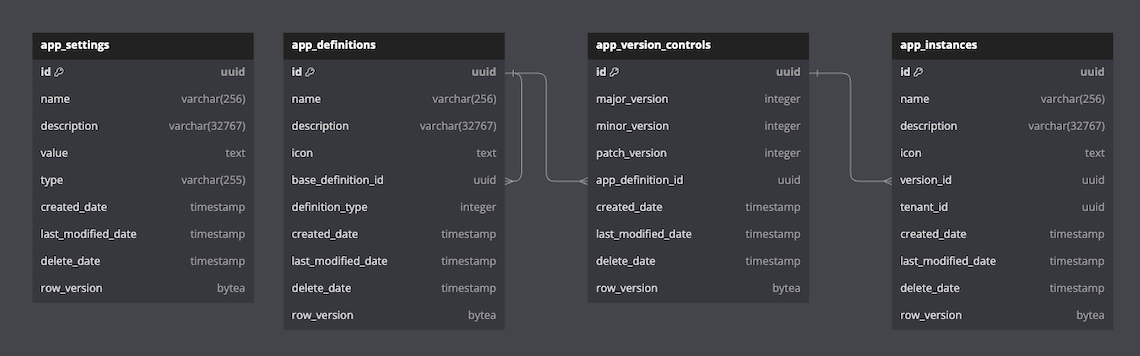
\includegraphics[width=\linewidth]{Images/model_core.png}
  \vspace{1em}
  \caption{The Core Model}
\end{figure}

Once the core functionalities are established, we shift our focus to security
with the identity model. This model is dedicated to managing user authentication and
authorization. It ensures that access to the information and functionalities
defined in core model is securely controlled. By integrating Identity model, we
discuss how the system protects sensitive data and operations from unauthorized
access, ensuring that users can interact with the core components in a secure
environment. This model not only reinforces the security of the system but also
defines user roles and permissions, which are essential for a multi-user
application. 
\begin{figure}[H]
  \centering
  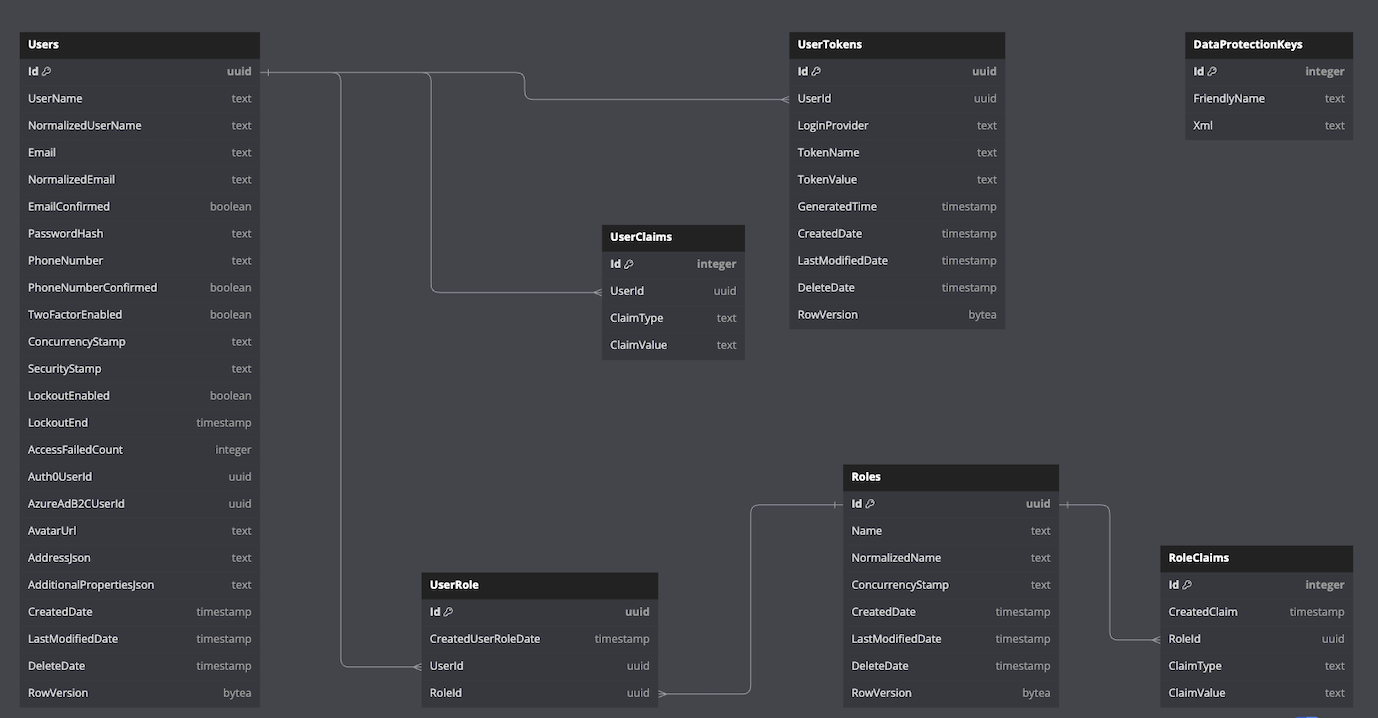
\includegraphics[width=\linewidth]{Images/model_auth.png}
  \vspace{1em}
  \caption{The Identity Model}
\end{figure}

Finally, we explore the form model, which ties the user interface and
interaction directly to the underlying data structures of the core model and the
security protocols of the Identity model. This model addresses how users will
experience and interact with the application through various forms and
interfaces. It encompasses everything from data entry and management to ensuring
that user interactions are intuitive and efficient. form model is critical for
defining the presentation and accessibility of the system’s features, making
sure that the application is not only functional and secure but also
user-friendly and responsive to the needs of its users.
\begin{figure}[H]
  \centering
  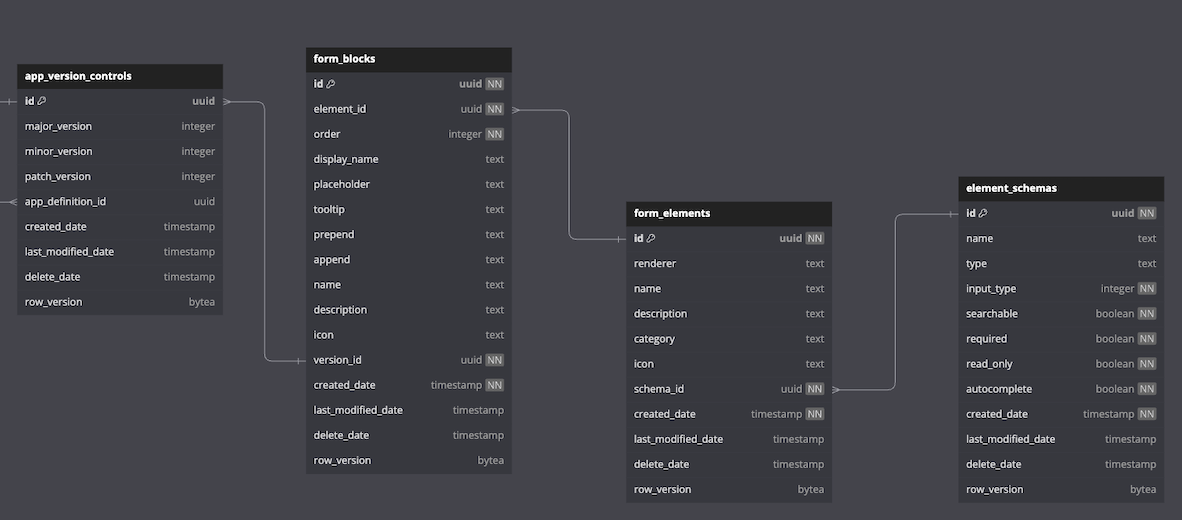
\includegraphics[width=\linewidth]{Images/model_form.png}
  \vspace{1em}
  \caption{The Form Model}
\end{figure}

By examining these models in this order, we effectively build from the internal
architecture to the external user interface, providing a comprehensive view of
the system's design from the ground up. This approach helps in understanding how
each component is interlinked and why each is vital to the overall success and
operability of the application.
\subsection{Blob storage}
As an intermediary entity situated between the data producers, exemplified by
the radar center, and the data consumers, represented by the Data Model and
Machine Learning team, our paramount responsibility lies in ensuring that the
data management infrastructure is meticulously designed to seamlessly
accommodate the diverse and often contrasting requirements set forth by both
parties.

The dataset, procured from the esteemed Nha Be radar center, adheres to the
rigorous SIGMET format, as delineated in \ref{sigmet}. This format encompasses a
plethora of scalar values pertaining to metadata facets such as the radar's
nomenclature, the modality of scanning employed, and the temporal stamp denoting
the execution of the scan. Concurrently, this data corpus embodies a rich array
of multidimensional metrics encapsulating various meteorological phenomena,
including but not limited to reflectivity and energy profiles.

Collaborative engagements with the modeling cadre, predominantly comprising
members from the distinguished teams led by Tu and Vinh, have endowed us with a
nuanced understanding of their exigencies and prerequisites vis-à-vis data
structuring paradigms. From the purview of these erudite teams, data
representation assumes two principal manifestations. Firstly, there is a
pronounced inclination towards encapsulating data in the form of images tailored
to specific geographical demarcations within the Vietnamese domain. A
quintessential exemplar of this utilization paradigm is elucidated in Figure
\ref{fig:nha-be-viz-far}, which encapsulates the data instrumental in honing the
multimodal solutions. Alternatively, there exists a proclivity towards direct
data consumption in the form of NumPy Tensors, leveraging the expansive spectrum
of NumPy-compatible APIs inclusive of those furnished by SciPy and XArray.
Although ostensibly more efficient, this mode of data consumption has not
garnered widespread adoption within the precincts of our collaborative endeavor.

Armed with an exhaustive comprehension of the requisites delineated by both
stakeholders and guided by heuristic principles germane to the architecture of
rudimentary data warehousing systems, we proffer a set of salient properties
that our envisaged system ought to embody:

Primarily, the envisaged data repository must find its abode in an Object
Storage medium, characterized by maximal interoperability with extant systems.
This necessitates the exclusion of proprietary solutions such as Google Cloud
Storage or Azure Storage Blob in favor of alternatives such as Hadoop
Distributed File System (HDFS) \cite{HDFS} or any Object Storage infrastructure
compliant with AWS S3 protocols. While HDFS presents itself as a viable
candidate, the logistical intricacies entailed in deploying and administering a
comprehensive HDFS cluster militate against prioritizing its adoption.
Fortuitously, our discerning team has identified a panacea in the form of MinIO,
an open-source Object Storage solution that not only aligns with the requisites
of our project but also boasts compatibility with prevailing AWS S3 APIs.

The conundrum surrounding the optimal data format to be stored within the Object
Storage reservoir has been a subject of fervent debate and contention amongst
our learned colleagues. While proponents of denormalization advocate for its
adoption to streamline data retrieval processes, empirical evidence underscores
the efficacy of the RAW data format in compressing and storing multidimensional
datasets, as attested by the diminutive file sizes characteristic of individual
scan executions. Indeed, attempts to transmute this format into alternative
structures, such as JSON, have yielded negligible dividends owing to the
intrinsic complexity of the dataset. Moreover, with the ascendancy of multimodal
Machine Learning paradigms, necessitating the simultaneous retrieval of diverse
data fields to facilitate batch processing, the retention of all pertinent
fields within a singular RAW file emerges as a prescient strategy poised to
accommodate the evolutionary trajectory of our modeling endeavors.

In delineating a nomenclatural schema for the files ensconced within the Object
Storage repository, precedence is accorded to a rudimentary ordering scheme
premised on tenant identification and temporal demarcation. For the myriad
utilization scenarios contemplated heretofore, the concatenation of the tenant
identifier with a timestamp proves to be a judicious nomenclatural convention.
Furthermore, the hierarchical organization of files within the Object Storage
framework ought to be predicated on a delineation between tenant-specific
directories and temporal partitions.

Regarding the temporal component of the nomenclatural schema, adherence to the
ISO-8601 standard, a globally ratified temporal convention, is deemed
imperative. The employment of the ISO-8601 timestamp format, typified by the
concatenation of year, month, day, hour, minute, and second components devoid of
any superfluous delimiters, serves to obviate compatibility issues with extant
filesystems. Notably, the conspicuous absence of special characters such as
hyphens and colons serves to circumvent prohibitions imposed by certain
filesystems, such as Windows, on the usage of such characters within filenames.

\section{System Architecture}
\begin{figure}[H]
    \centering
    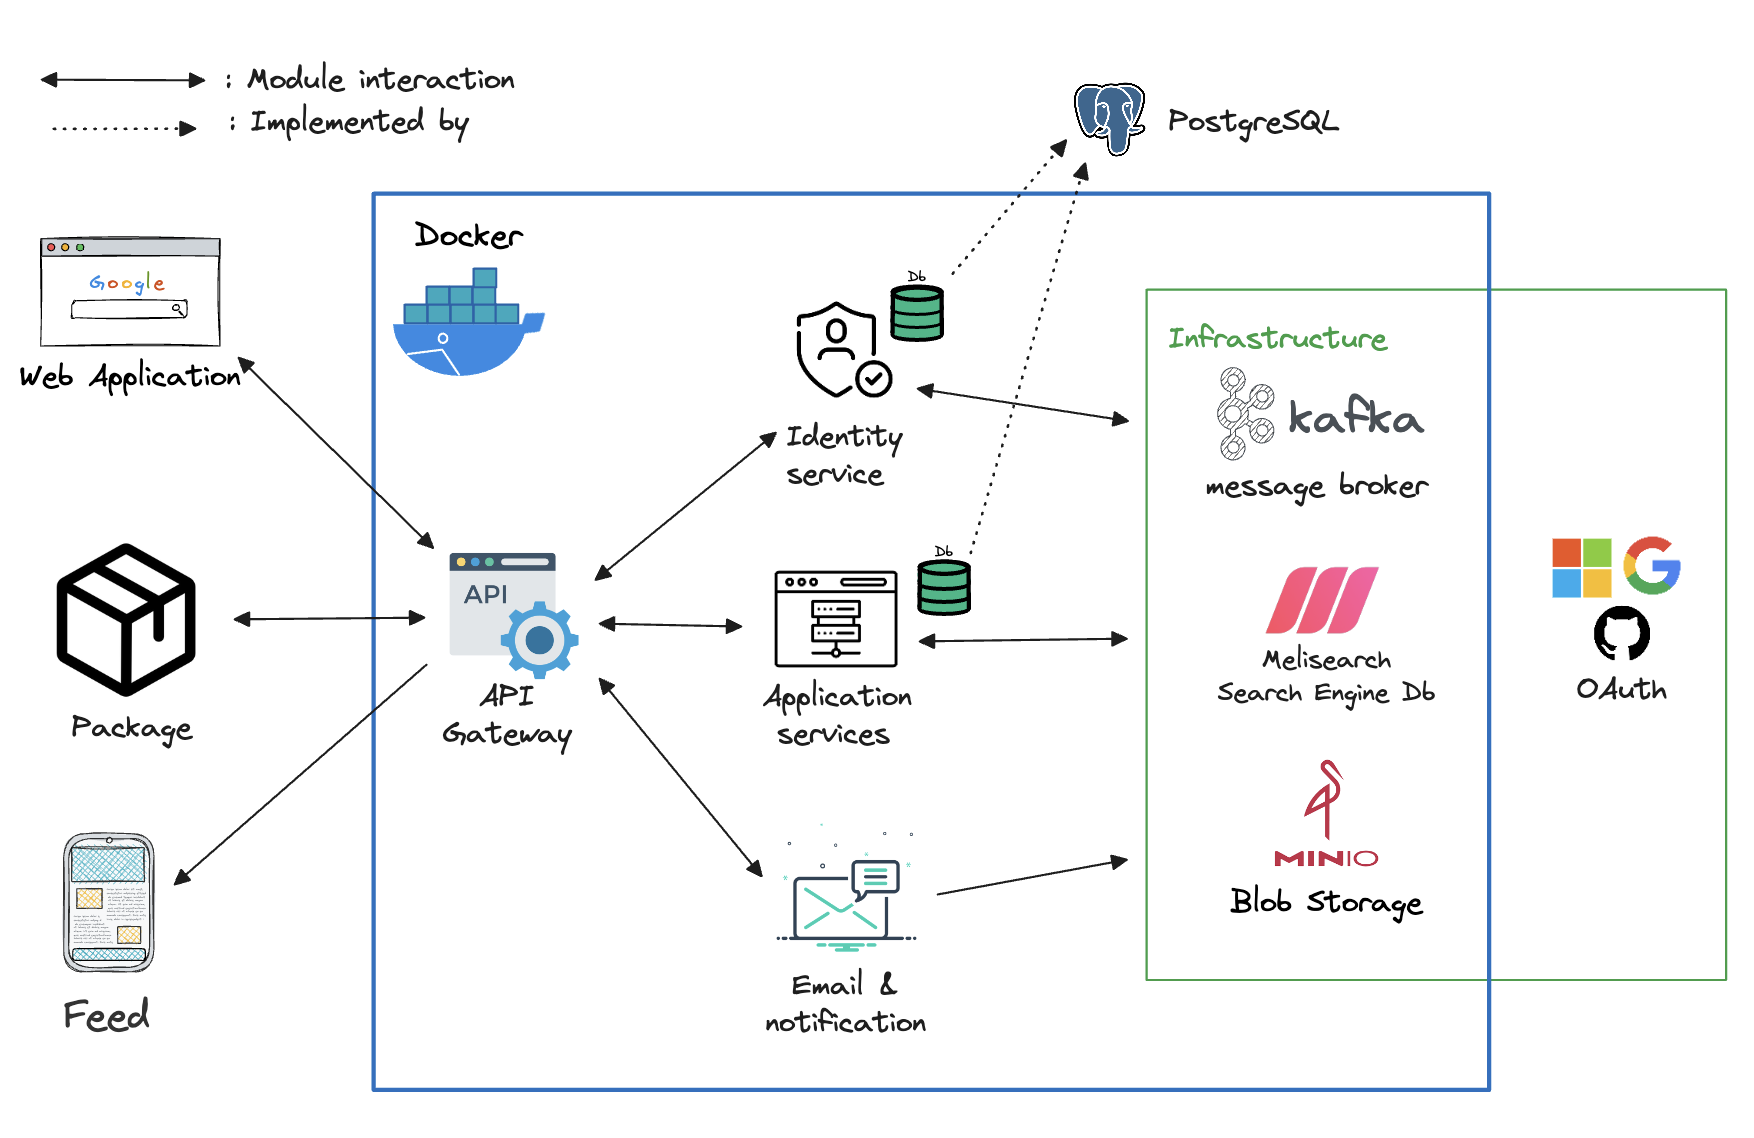
\includegraphics[width=\linewidth]{Images/arch.png}
    \vspace{1em}
    \caption{System Architecture}
    \label{fig:sow}
\end{figure}
\vspace{0.5cm}
Based on the requirements set by stakeholders and after studying the existing
system, the team proposes the design and implementation of a Weather Data Platform. Figure
\ref{fig:sow} illustrates the implementation of the system.
\newpage

\subsection{Microservices}

In essence, a microservices architecture decomposes a large software application
into a collection of smaller, self-contained services. Each service plays a
specific role and owns a well-defined business capability. These services are
loosely coupled, meaning they interact through well-designed APIs and operate independently.

Microservices architectures offer a compelling approach to building software. By
decomposing large applications into smaller, independent services, they unlock
agility, maintainability, and fault isolation.  Each service owns a specific
business function and interacts with others through well-defined APIs. This
allows for faster development cycles, easier maintenance of individual services,
and the freedom to choose the best technology for each job.

However, this power comes with a price. Managing a distributed system with
numerous services inherently increases complexity compared to a monolithic
application. Communication between services adds overhead to the system's
performance. Perhaps the most significant challenge lies in ensuring data
consistency across these independent services, requiring meticulous design and
implementation.  Carefully considering these trade-offs is crucial before
embarking on a microservices journey.

While microservices boast impressive agility and maintainability, adopting this
architecture isn't without its complexities.  Managing a distributed system with
numerous services inherently increases complexity compared to a monolithic
application.  Furthermore, communication between these services adds overhead to
the system's performance.  Perhaps the most significant challenge lies in
ensuring data consistency across these independent services, requiring
meticulous design and implementation.

\subsection{Clean Architecture}

Microservices and Clean Architecture can complement each other to create a
modular, maintainable, and scalable system. Microservices architecture promotes
the development of small, independent services that can be deployed, scaled, and
updated independently. Each microservice encapsulates a specific business
capability or domain, reducing the overall complexity of the system.

Clean Architecture, on the other hand, advocates for a layered approach to
software design, promoting separation of concerns and decoupling of components.
By adhering to the principles of Clean Architecture within each microservice,
developers can achieve a high degree of modularity, testability, and
maintainability.

Clean Architecture separates the system into distinct layers, each with specific
responsibilities. The Shared Kernel acts as the core, housing reusable
components that benefit all layers. The Domain layer sits at the heart of the
application, defining core entities and their behaviors. A common base class
promotes code maintainability within this layer. The Application layer
orchestrates request routing and establishes project-wide contracts for
implementation in other layers. Clean Architecture emphasizes the testability of
each layer through unit tests. Frameworks like xUnit simplify unit test
creation. 

The Infrastructure layer provides supporting services for the application.
Cross-cutting concerns like logging reside here. User registration,
authentication, and authorization functionalities are handled by the Identity
layer. Persistence takes care of data access using patterns like repositories
and Unit of Work. The Web Framework layer manages configurations for the web
application, while the Web API layer delivers functionality to the user.
Finally, plugins bridge the gap between monolithic and microservices
architectures by promoting modularity.



\newpage
\chapter{Implementation}
\section{Data Processing}
The implementation phase of the team will be an extension to the current system,
which is outlined in Figure \ref{fig:sow}.

In step 3, the team will set up a simple SFTP server. SFTP is a straightforward
and widely used protocol, supported by numerous libraries and tools for
communication based on this protocol. Additionally, compared to FTP, the
mentioned protocol ensures security during data transfer. Depending on the
permissions, the team may assist the observation station in constructing scripts
to automatically forward processed files or allow manual file submission.

Once files are uploaded to the SFTP server, the team utilizes Airflow to
orchestrate all existing ETL workflows in the overall system. Currently, the
team pauses with a single DAG to process data from the Nha Be observation
station. Airflow monitors newly added files on our SFTP server and initiates the
ETL process. The choice of Apache Spark is based on the volume and complexity of
the data. If the data size per new SIGMET file is manageable with Python alone,
without the need for Spark, it will not be employed in this step.

Meteorological data, upon reaching the team's infrastructure, will be bifurcated
into two main streams: Metadata, such as creation date, size, timestamp, etc.,
will be stored in a traditional Relational Database Management System (RDBMS).
Specifically, PostgreSQL is chosen due to its popularity and the team's
familiarity. Storing metadata here facilitates rapid query responses without
direct access to the raw data. Common queries may include:

\begin{itemize}
    \item What timestamps are being recorded? (e.g., from 21/11/2023 to
    17/12/2023)
    \item At timestamp $x$, what are the geographical coordinates of the radar?
    \item What fields of data are currently stored?
\end{itemize}

Additionally, the database acts as an index, quickly identifying the storage
location of raw data.

For specific hydrometeorological data, the team finds it inefficient to store
them directly in conventional DBMS. Simultaneously, storing data in files still
maintains a reasonable overall size. Therefore, the team decides to separate the
raw data and store it directly in files. This approach, combined with the
previously mentioned indexes, accelerates the retrieval process.

To facilitate data queries for models, machine learning, AI, etc., the team will
develop a simple backend server using Python's FastAPI at step 5. In step 6, the
backend receives query data in REST API format, queries the metadata DB and data
files, and returns the achieved results. During different training instances,
Machine Learning entities can connect to this server to retrieve data.

It's worth mentioning that the entire system will be developed and operated in a
containerized manner and will be deployed on the Kubernetes platform. This
reflects the system's ability to maintain high availability and ease of solution
maintenance. In this illustration, the team will deploy it on a cluster of
Raspberry Pi-embedded computers.

Lastly, in step 7, the team proposes an additional consideration. If suitable,
the team may build a DataLoader to swiftly serve other model-making groups.
Considering the popularity of Pytorch in AI, the team will initially approach
this platform.

\section{System}

\subsection{Programming languages and Libraries}

C\# was selected for this project because of its widespread popularity in
enterprise applications and its capability to operate across various operating
systems following the release of .NET Core. This feature significantly enhances
deployment flexibility, allowing the application to be utilized in diverse
environments. 

Additionally, we have incorporated ASP.NET Core specifically version 8 into our
technology stack. By leveraging ASP.NET Core, we benefit from a robust,
well-supported framework that facilitates the development of scalable and secure
web applications. It seamlessly integrates with C\#, enabling us to utilize a
consistent programming environment while also exploiting features such as
dependency injection, a vast ecosystem of middleware, and a strong configuration
system that is suited to modern web applications.

ASP.NET Core 8 brings forward improvements in areas such as minimized startup
times, reduced memory footprint, and enhanced security features, making it an
ideal choice for developing scalable and secure web applications. The choice
also underscores our commitment to developing applications that are both
efficient and future-proof, ensuring that they perform optimally on both Windows
and non-Windows platforms. This alignment with .NET Core’s cross-platform
capabilities ensures that our project remains versatile and adaptable to the
evolving technological landscape.

Optionally, we have integrated the Nuxt framework into our technology stack.
Nuxt is a progressive Vue framework that is used for building more robust and
versatile web applications. It simplifies the development process by handling
various aspects of the web infrastructure, such as server-side rendering, static
site generation, and automatic code splitting. This inclusion enriches our
application's interactivity and user experience, providing a seamless and
dynamic interface for users.

\subsection{Command Query Responsibility Segregation}

The Command Query Responsibility Segregation (CQRS) is an architectural pattern
that distinctively separates the tasks of reading data (queries) and writing
data (commands) within a software application. This separation splits
responsibilities into two main components:

\begin{itemize}
\item \textbf{Command Side}: This component manages operations that modify the
system's state. It handles incoming commands from clients or external systems,
conducts validations, and updates the data store accordingly. This side is
essential for maintaining the integrity and accuracy of data modifications
within the application.
\item \textbf{Query Side}: Dedicated to data retrieval, this component processes
all read requests. It fetches data from the appropriate sources, ensuring that
the information provided is accurate and reflects the current state of the data
store.
\end{itemize}

Key advantages of employing the CQRS pattern are:

\begin{itemize}
\item \textbf{Scalability}: CQRS allows for the independent scaling of the read
and write components based on their respective workloads, which can
significantly enhance system performance.
\item \textbf{Flexibility}: With the separation of concerns, different storage
and optimization strategies can be applied to the reading and writing processes.
This flexibility enables the use of the most appropriate tools for each
function, optimizing efficiency.
\item \textbf{Event-Driven Architecture Compatibility}: The use of CQRS often
complements event-driven architectures, where changes in the system's state are
captured and managed as events. This compatibility ensures that the architecture
is dynamic and responsive to changes in business requirements.
\end{itemize}

\subsection{Project Structure}

\begin{figure}[H]
  \centering
  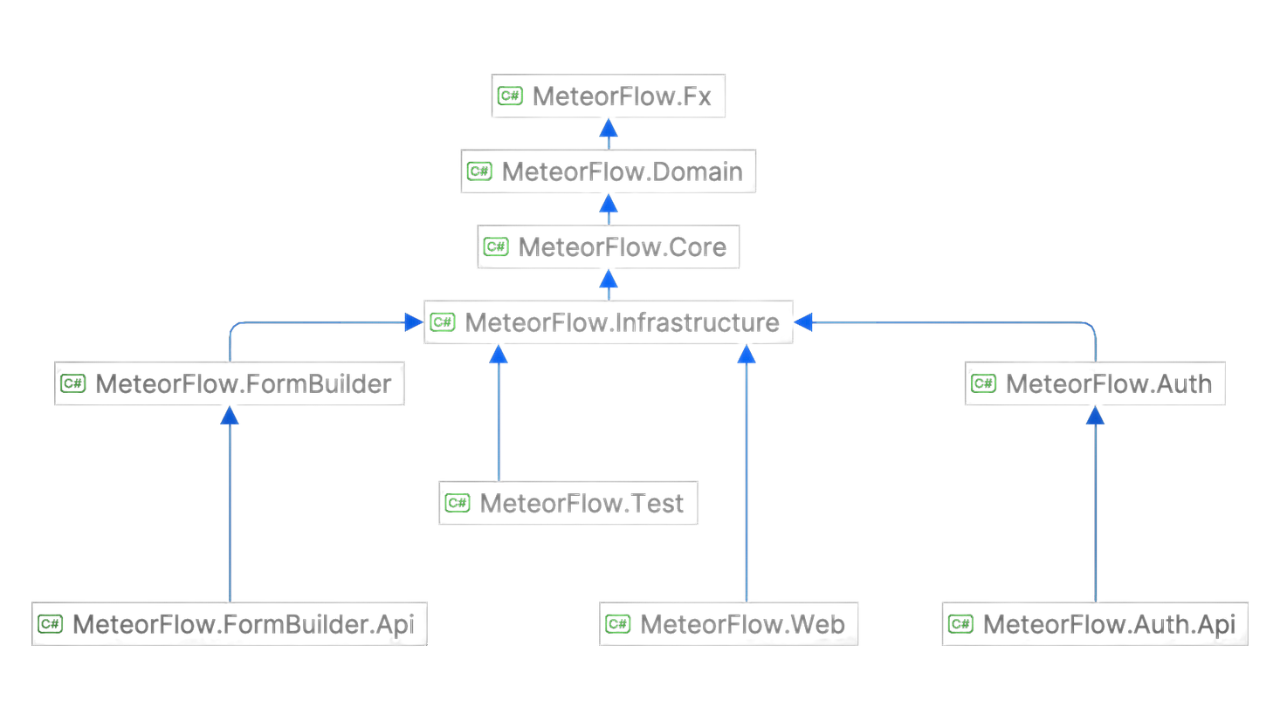
\includegraphics[width=\linewidth]{Images/ProjectDir.png}
  \caption{Project Structure}
\end{figure}

MeteorFlow is depicted as a modular framework comprising several interdependent
components. Each library or module serves a distinct function, collectively
supporting a robust and scalable application infrastructure. This section will
delineate the roles and relationships of these components.

MeteorFlow.Fx enriches the application by introducing additional functionalities
or user interface enhancements. These features, while not central to the primary
business logic, significantly augment the application’s overall capabilities,
providing enriched user experiences and functional extensions.

MeteorFlow.Domain is tailored to articulate the business domain, encapsulating
entities and rules essential to the application's domain logic. Its reliance on
the Core module underscores the latter’s foundational role within the
architecture, affirming its influence over the domain-specific functionalities.

At the heart of the architecture, MeteorFlow.Core embodies the fundamental
business logic and operations critical to the application. Its pivotal role is
underscored by its influence on all peripheral modules, which depend on the Core
for their foundational functionalities.

MeteorFlow.Infrastructure functions as the backbone for data access and manages
cross-cutting concerns such as logging and caching. This module is crucial for
the operational management of the application, interfacing seamlessly with the
Core module to apply essential functionalities across various infrastructural
tasks.

Built upon the MeteorFlow.Infrastructure, the Auth module specializes in
security and authentication processes, managing user verification and credential
handling. The module provides APIs to enable external access to their functionalities and
seamlessly integrate with other systems and applications. Other modules
currently or in the near future follow the same structure above to provide
additional functionalities.

MeteorFlow.Web, primarily tasked with managing the application’s API gateway,
interacts with all other modules within MeteorFlow to ensure robust web
operations and effective resource management. Its role is crucial in maintaining
the integrity and performance of web-based services, underpinning the system's
interaction with users and external systems.



\section{API Specification}
\subsection{Core API}

\subsubsection*{GET /api/core/definition}
\begin{longtable}{|>{\raggedright\arraybackslash}p{3cm}|p{10cm}|}
\hline
\textbf{Tags} & Definition \\
\hline
\textbf{Description} & Retrieves a list of all core definitions. \\
\hline
\textbf{Responses} & 200: An array of core definitions returned successfully. \\
 & 401: Unauthorized access. \\
\hline
\end{longtable}

\subsubsection*{POST /api/core/definition}
\begin{longtable}{|>{\raggedright\arraybackslash}p{3cm}|p{10cm}|}
\hline
\textbf{Tags} & Definition \\
\hline
\textbf{Description} & Creates a new core definition. \\
\hline
\textbf{Request Body} & AppDefinitions schema. \\
\hline
\textbf{Responses} & 201: Core definition created successfully. \\
 & 400: Bad request if the data is invalid. \\
 & 401: Unauthorized access. \\
\hline
\end{longtable}

\subsubsection*{GET /api/core/definition/\{id\}}
\begin{longtable}{|>{\raggedright\arraybackslash}p{3cm}|p{10cm}|}
\hline
\textbf{Tags} & Definition \\
\hline
\textbf{Description} & Retrieves a specific core definition by ID. \\
\hline
\textbf{Parameters} & id: UUID of the core definition. \\
\hline
\textbf{Responses} & 200: Core definition returned successfully. \\
 & 404: Core definition not found. \\
 & 401: Unauthorized access. \\
\hline
\end{longtable}

\subsubsection*{DELETE /api/core/definition/\{id\}}
\begin{longtable}{|>{\raggedright\arraybackslash}p{3cm}|p{10cm}|}
\hline
\textbf{Tags} & Definition \\
\hline
\textbf{Description} & Deletes a specific core definition by ID. \\
\hline
\textbf{Parameters} & id: UUID of the core definition. \\
\hline
\textbf{Responses} & 200: Core definition deleted successfully. \\
 & 404: Core definition not found. \\
 & 401: Unauthorized access. \\
\hline
\end{longtable}

\subsubsection*{POST /api/core/instance}
\begin{longtable}{|>{\raggedright\arraybackslash}p{3cm}|p{10cm}|}
\hline
\textbf{Tags} & Instance \\
\hline
\textbf{Description} & Creates a new instance. \\
\hline
\textbf{Request Body} & AppInstances schema. \\
\hline
\textbf{Responses} & 201: Instance created successfully. \\
 & 400: Bad request if the data is invalid. \\
 & 401: Unauthorized access. \\
\hline
\end{longtable}

\subsubsection*{GET /api/core/instance/\{id\}}
\begin{longtable}{|>{\raggedright\arraybackslash}p{3cm}|p{10cm}|}
\hline
\textbf{Tags} & Instance \\
\hline
\textbf{Description} & Retrieves a specific instance by ID. \\
\hline
\textbf{Parameters} & id: UUID of the instance. \\
\hline
\textbf{Responses} & 200: Instance returned successfully. \\
 & 404: Instance not found. \\
 & 401: Unauthorized access. \\
\hline
\end{longtable}

\subsubsection*{DELETE /api/core/instance/\{id\}}
\begin{longtable}{|>{\raggedright\arraybackslash}p{3cm}|p{10cm}|}
\hline
\textbf{Tags} & Instance \\
\hline
\textbf{Description} & Deletes a specific instance by ID. \\
\hline
\textbf{Parameters} & id: UUID of the instance. \\
\hline
\textbf{Responses} & 200: Instance deleted successfully. \\
 & 404: Instance not found. \\
 & 401: Unauthorized access. \\
\hline
\end{longtable}

\subsubsection*{GET /api/core/setting}
\begin{longtable}{|>{\raggedright\arraybackslash}p{3cm}|p{10cm}|}
\hline
\textbf{Tags} & Setting \\
\hline
\textbf{Description} & Retrieves a list of all settings. \\
\hline
\textbf{Responses} & 200: An array of settings returned successfully. \\
 & 401: Unauthorized access. \\
\hline
\end{longtable}

\subsubsection*{POST /api/core/setting}
\begin{longtable}{|>{\raggedright\arraybackslash}p{3cm}|p{10cm}|}
\hline
\textbf{Tags} & Setting \\
\hline
\textbf{Description} & Creates a new setting. \\
\hline
\textbf{Request Body} & AppSettings schema. \\
\hline
\textbf{Responses} & 201: Setting created successfully. \\
 & 400: Bad request if the data is invalid. \\
 & 401: Unauthorized access. \\
\hline
\end{longtable}

\subsubsection*{GET /api/core/setting/\{id\}}
\begin{longtable}{|>{\raggedright\arraybackslash}p{3cm}|p{10cm}|}
\hline
\textbf{Tags} & Setting \\
\hline
\textbf{Description} & Retrieves a specific setting by ID. \\
\hline
\textbf{Parameters} & id: UUID of the setting. \\
\hline
\textbf{Responses} & 200: Setting returned successfully. \\
 & 404: Setting not found. \\
 & 401: Unauthorized access. \\
\hline
\end{longtable}

\subsubsection*{DELETE /api/core/setting/\{id\}}
\begin{longtable}{|>{\raggedright\arraybackslash}p{3cm}|p{10cm}|}
\hline
\textbf{Tags} & Setting \\
\hline
\textbf{Description} & Deletes a specific setting by ID. \\
\hline
\textbf{Parameters} & id: UUID of the setting. \\
\hline
\textbf{Responses} & 200: Setting deleted successfully. \\
 & 404: Setting not found. \\
 & 401: Unauthorized access. \\
\hline
\end{longtable}

\subsubsection*{GET /configuration}
\begin{longtable}{|>{\raggedright\arraybackslash}p{3cm}|p{10cm}|}
\hline
\textbf{Tags} & FileConfiguration \\
\hline
\textbf{Description} & Retrieves the current configuration. \\
\hline
\textbf{Responses} & 200: Configuration returned successfully. \\
 & 401: Unauthorized access. \\
\hline
\end{longtable}

\subsubsection*{POST /configuration}
\begin{longtable}{|>{\raggedright\arraybackslash}p{3cm}|p{10cm}|}
\hline
\textbf{Tags} & FileConfiguration \\
\hline
\textbf{Description} & Updates the current configuration. \\
\hline
\textbf{Request Body} & FileConfiguration schema. \\
\hline
\textbf{Responses} & 200: Configuration updated successfully. \\
 & 400: Bad request if the data is invalid. \\
 & 401: Unauthorized access. \\
\hline
\end{longtable}

\subsection{Indentity API}

\subsubsection*{GET /api/auth}
\begin{longtable}{|>{\raggedright\arraybackslash}p{3cm}|p{10cm}|}
\hline
\textbf{Tags} & Auth \\
\hline
\textbf{Description} & Retrieves authentication status based on the returnUrl parameter. \\
\hline
\textbf{Parameters} & returnUrl (string): The URL to return to after authentication. \\
\hline
\textbf{Responses} & 200: Authentication status returned successfully. \\
\hline
\end{longtable}

\subsubsection*{POST /api/auth/login}
\begin{longtable}{|>{\raggedright\arraybackslash}p{3cm}|p{10cm}|}
\hline
\textbf{Tags} & Auth \\
\hline
\textbf{Description} & Logs in a user with provided credentials. \\
\hline
\textbf{Request Body} & LoginInfo schema: Includes username and password. \\
\hline
\textbf{Responses} & 200: Login successful. \\
\hline
\end{longtable}

\subsubsection*{POST /api/users/\{id\}/passwordresetemail}
\begin{longtable}{|>{\raggedright\arraybackslash}p{3cm}|p{10cm}|}
\hline
\textbf{Tags} & Users \\
\hline
\textbf{Description} & Sends a password reset email to the user specified by ID. \\
\hline
\textbf{Parameters} & id (string, uuid): Unique identifier of the user. \\
\hline
\textbf{Responses} & 200: Password reset email sent successfully. \\
\hline
\end{longtable}

\subsubsection*{PUT /api/users/\{id\}/password}
\begin{longtable}{|>{\raggedright\arraybackslash}p{3cm}|p{10cm}|}
\hline
\textbf{Tags} & Users \\
\hline
\textbf{Description} & Updates the password for the user specified by ID. \\
\hline
\textbf{Parameters} & id (string, uuid): Unique identifier of the user. \\
\hline
\textbf{Request Body} & PasswordSetter schema: Includes new password and confirmation. \\
\hline
\textbf{Responses} & 200: Password updated successfully. \\
 & 404: User not found. \\
\hline
\end{longtable}

\subsubsection*{POST /api/users/\{id\}/emailaddressconfirmation}
\begin{longtable}{|>{\raggedright\arraybackslash}p{3cm}|p{10cm}|}
\hline
\textbf{Tags} & Users \\
\hline
\textbf{Description} & Sends an email confirmation to the user specified by ID. \\
\hline
\textbf{Parameters} & id (string, uuid): Unique identifier of the user. \\
\hline
\textbf{Responses} & 200: Email confirmation sent successfully. \\
\hline
\end{longtable}
\section{Datastore}
\subsection{The purpose of storing data directly as raw file}
In the comprehensive compilation acquired during the recent field excursion, an
array of invaluable data was meticulously gathered, meticulously chronicled, and
thoughtfully analyzed. Specifically, our focus gravitated towards the
operational activities conducted within the radar center situated in the Nha Be
district. Operating at the pinnacle of technological advancement, the radar
center diligently executes periodic scans of the atmospheric conditions,
facilitating the meticulous documentation and exportation of a SIGMET file,
which serves as a repository encapsulating a myriad of meteorological phenomena
and atmospheric dynamics.

The SIGMET file, serving as the quintessential embodiment of scientific rigor
and methodological precision, meticulously records a plethora of critical
parameters and meteorological variables. Among the salient features meticulously
delineated within this archival masterpiece are the discerning metrics of
reflectivity and wind radial velocity. Reflectivity, a fundamental metric in
radar meteorology, is an indispensable parameter delineating the intensity of
electromagnetic waves returned to the radar antenna from various atmospheric
particles, thereby furnishing crucial insights into the spatial distribution and
intensity of precipitation within the monitored region. Furthermore, the wind
radial velocity, an elemental component in meteorological analysis, delineates
the rate and direction of atmospheric motion along the radial axis relative to
the radar antenna. These metrics serve as a vital tool in elucidating the
intricate dynamics of atmospheric circulation, enabling meteorologists to
decipher prevailing wind patterns, identify regions of convective activity, and
forecast the trajectory of severe weather phenomena with enhanced accuracy and
precision.

Yet, amidst the effervescent tapestry of meteorological data acquisition and
analysis, a conundrum of paramount importance arises: the optimization of data
storage and retrieval mechanisms. It is within this crucible of inquiry that the
proposition to store meteorological results directly within the file repository
assumes a mantle of significance, heralding a paradigm shift in data management
practices.

Indeed, the inherent multidimensionality of meteorological data, encapsulated
within its tripartite tensor structure, underscores the imperative for a
streamlined approach to data storage and retrieval. By eschewing aggregation and
denormalization techniques, we advocate for a direct integration of results
within the archival framework, thereby fortifying the foundations of data
integrity and computational efficiency.

Moreover, the proposition to leverage the existing ETL (Extract, Transform,
Load) system developed by Vaisala, as utilized by our esteemed National Center
for Hydrometeorological Forecasting, emerges as a beacon of pragmatism and
resourcefulness. In a landscape fraught with technological complexities and
budgetary constraints, the utilization of pre-existing infrastructure represents
a judicious allocation of resources, affording seamless integration and
interoperability across disparate data management platforms.

In summation, the decision to store meteorological data directly within the file
repository, without resorting to further aggregation techniques, emerges as a
testament to both pragmatism and foresight. By embracing this approach, we not
only enhance the accessibility and usability of meteorological datasets but also
lay the groundwork for a new era of scientific inquiry and meteorological
prognostication, fortified by the pillars of technological innovation and
methodological rigor.


\subsection{Extracting data from each of the radar center}
We have authored a script, albeit not yet integrated into the operational
system, designed to facilitate the redirection of the SIGMET (Significant
Meteorological Information) file from the data center to our preconfigured
Storage Server.

Presently, the script is implemented in Python to ensure platform-agnosticism.
Accompanied by a concise setup script, it will be poised for execution on the
radar center's machinery.

MinIO has been employed as an unstructured data repository owing to its
compatibility with the S3 (Simple Storage Service) protocol. As the system
matures in the distant future, transitioning to AWS S3 should be
straightforward. The underlying logic and API for interfacing with the storage
infrastructure remain largely invariant during such a migration.

\begin{lstlisting}[language=Python, caption={Part of the script for uploading data to Storage}]
file_path = pathlib.Path(args.filename)

s3_client = boto3.client( "s3", endpoint_url=os.getenv("S3_HOSTNAME"),
    aws_access_key_id=os.getenv("S3_ACCESS_KEY_ID"),
    aws_secret_access_key=os.getenv("S3_SECRET_ACCESS_KEY"), ) _ =
    s3_client.upload_file(file_path, os.getenv("S3_BUCKET"),
    generate_new_name(file_path.name))
\end{lstlisting}

\setlength{\emergencystretch}{3em} % provides additional stretching to avoid
underfull hboxes

Currently, we follow a designated nomenclature for naming data files of the
RADAR objects: \texttt{<year><month><day>T<hour><minute><second>}. This system
enhances the speed of data retrieval for specific times of the day. Utilizing S3
Prefix filtering, we can efficiently select multiple data points within a time
frame that may vary from a second to an entire year.

For instance, to query data for a specific day (e.g., 2024-03-15), utilizing the
UNIX path wildcard, we can express our query as:

\begin{lstlisting}[language=sh]
ls 20240315T*
\end{lstlisting}

Analogously, the same query can be executed using the \texttt{boto3} library in
Python:

\begin{lstlisting}[language=Python, caption={Querying data in 2024-03-15}]
def query_with_wildcard(bucket_name): s3_client = boto3.client('s3')
    
    response = s3_client.list_objects_v2( Bucket='nha-be-radar',
        Prefix='20240315T' )
        
    return [obj['Key'] for obj in response['Contents']]
\end{lstlisting}

Moreover, although our naming convention deviates somewhat from the ISO-8601
standard for timestamp representation, the inclusion of the letter \textbf{T}
aids in swiftly identifying datetime components within the naming structure.

One limitation of this naming convention is its inability to support wildcard
querying for a central time component. Consider the scenario necessitating data
retrieval for a specific hour daily. Utilizing the UNIX wildcard, this can be
depicted as:

% Correct use of the lstlisting environment
\begin{lstlisting}[language=sh]
ls 202403*T09*
\end{lstlisting}

The utilization of an internal wildcard here implies the absence of an efficient
mechanism for querying such objects presently. The current recourse involves
maximal prefixing (e.g., \texttt{Prefix=202403}), followed by subsequent
filtering in Python.

\subsection{Data Explorer}
Besides S3-compatible API for accessing the storage, our solution also provides
some alternative ways for preview the data storage. This can be used for manual
intervention (in case of failure), or simply for the radar center's operators to
preview.

First, there is an online explorer that can be access from the web browser. As
you can see from Figure \ref{fig:minio-home}, the web UI is very user-friendly
and easy-to-use. With the use of IAM (shorts for Identity and Access Management)
and \textbf{Policies}, the admin user of our entire system can restrict what a
tenant (or a radar center) can see and what should be hidden.

\begin{figure}[H]
    \centering
    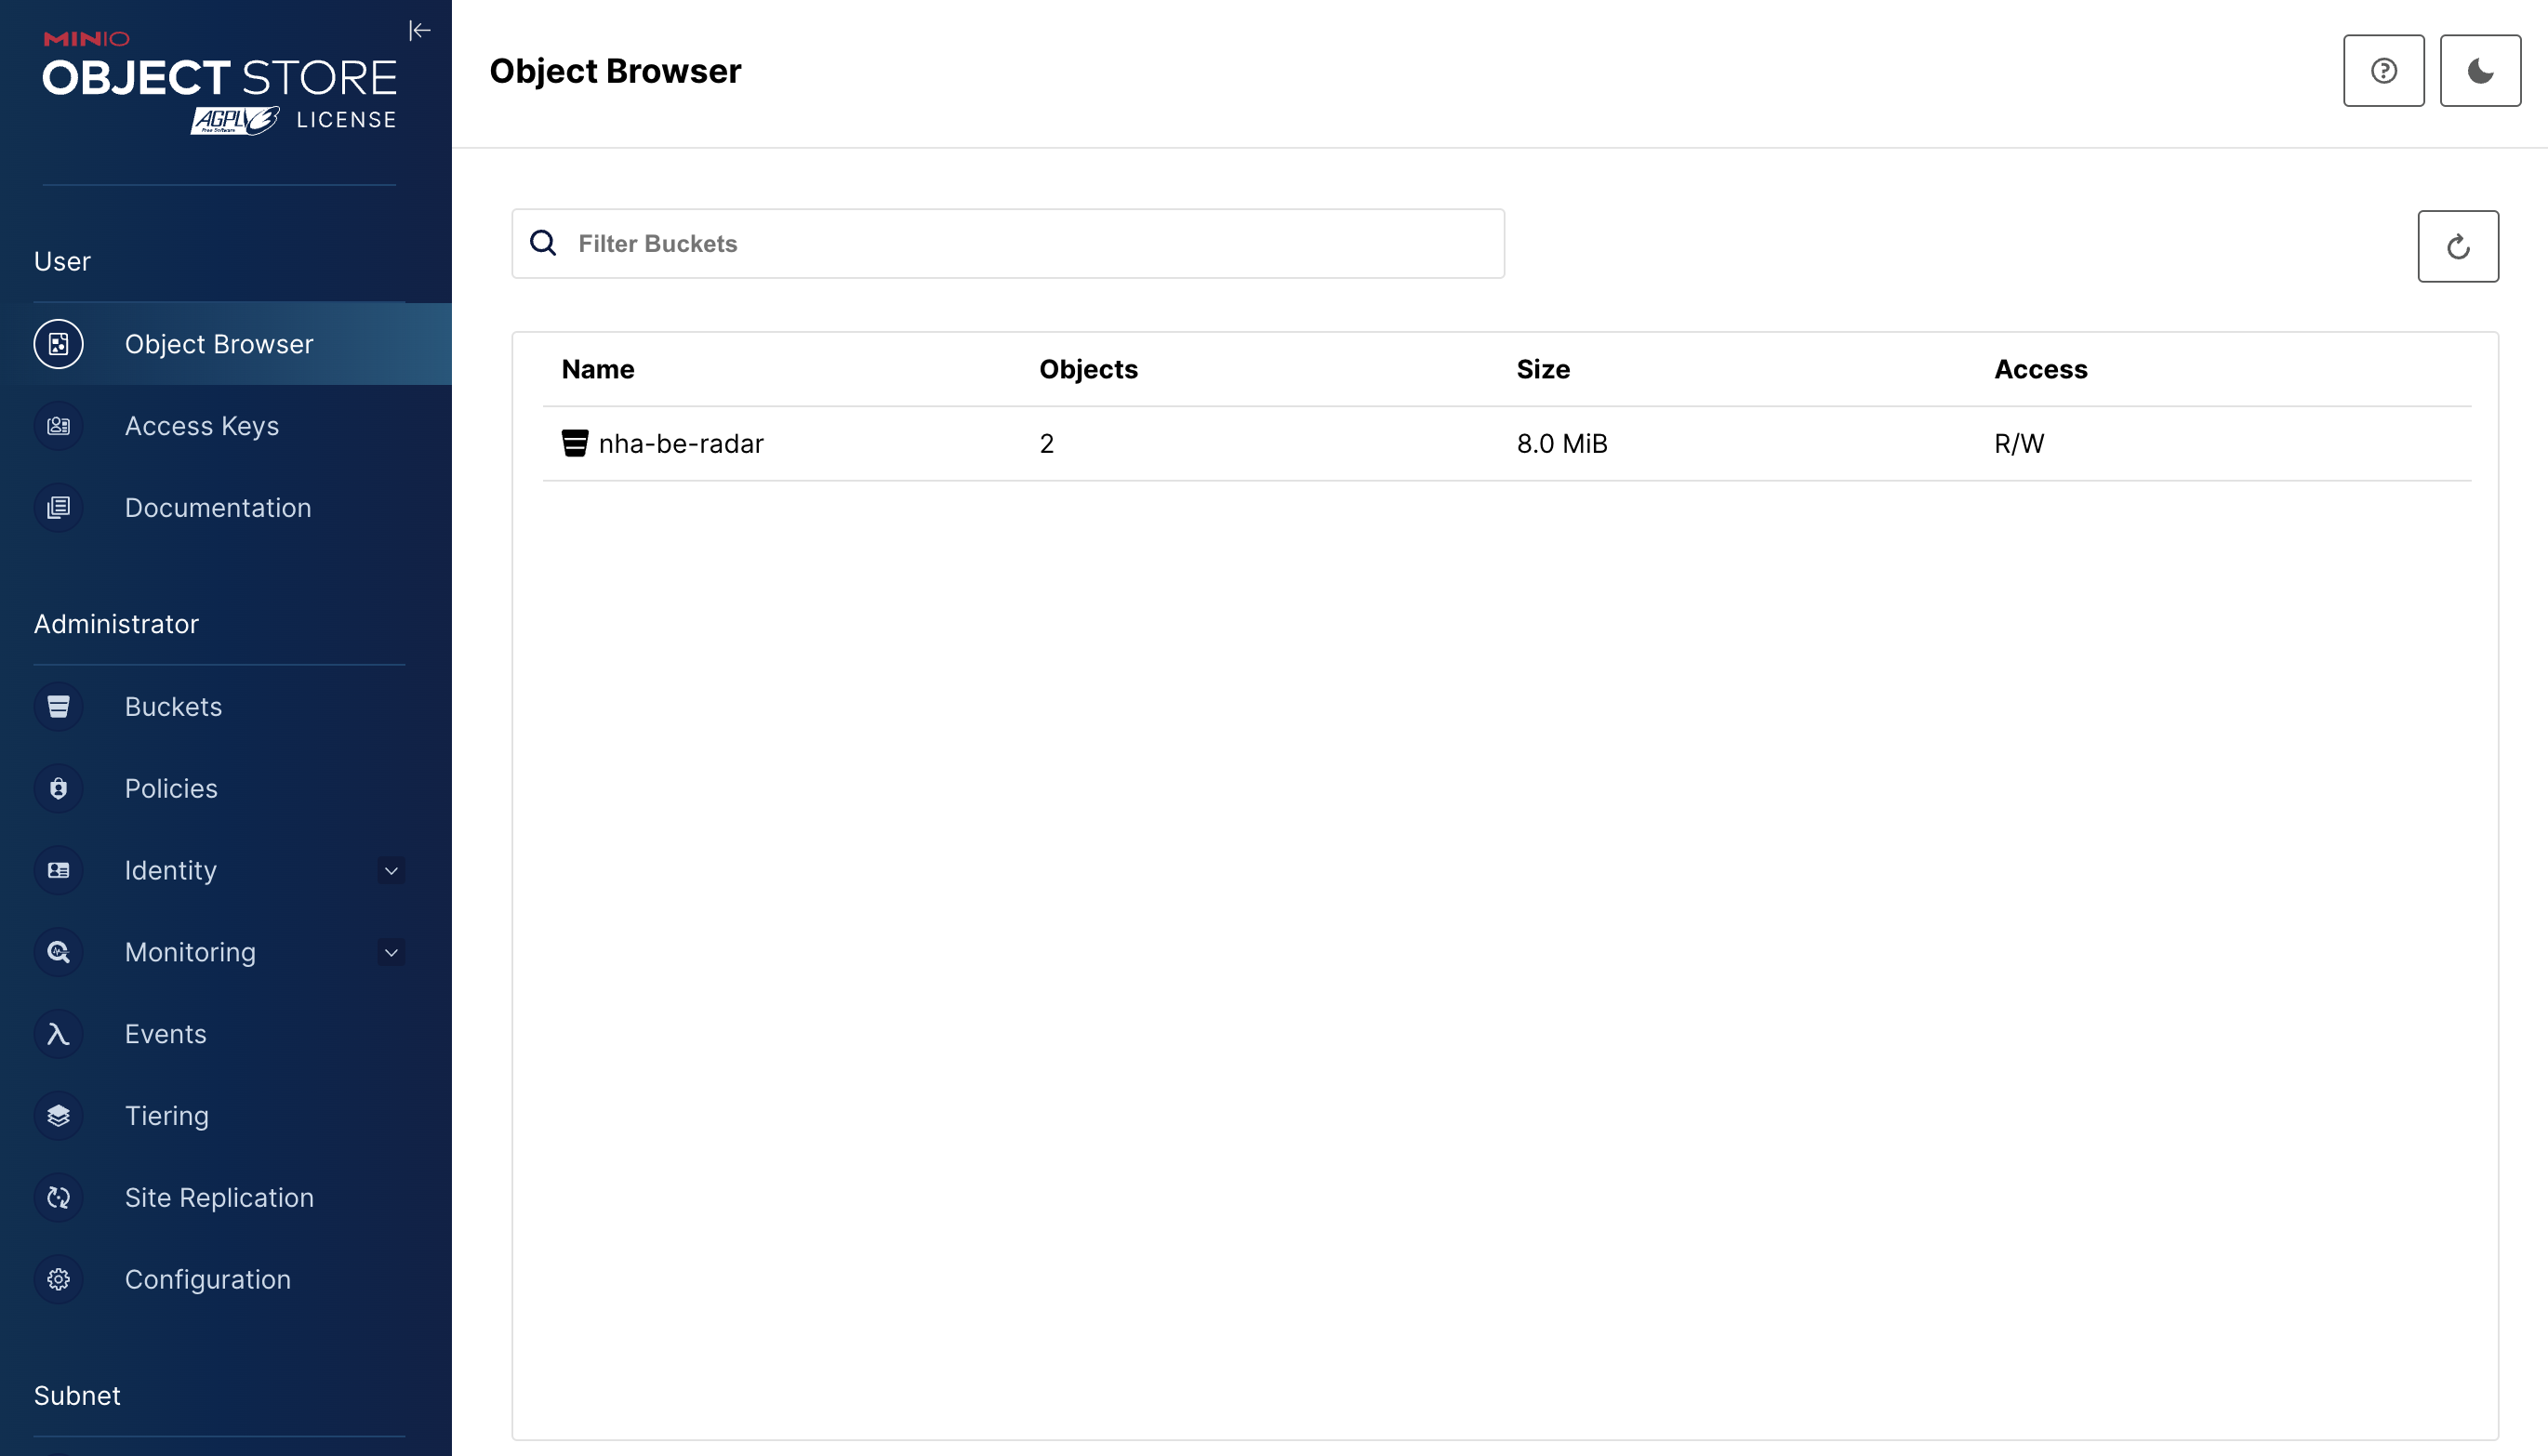
\includegraphics[width=0.8\linewidth]{Images/4.3-datastore/minio-bucket.png}
    \vspace{1em}
    \caption{MinIO web interface provides a clear and intuitive way to explore the storage}
    \label{fig:minio-home}
\end{figure}

Currently, as of the time of writing, our system has been self-hosted on a small
Raspberry Pi server. The explorer has been set up with necessary load balancing,
DNS and SSL/TLS registering correctly. Anyone that has been given proper
permissions can visit \url{https://explorer.meteor-flow.com/} to see the server
running. Figure \ref{fig:minio-files} shows some of the files that our team has
prepared beforehand.

\begin{figure}[H]
    \centering
    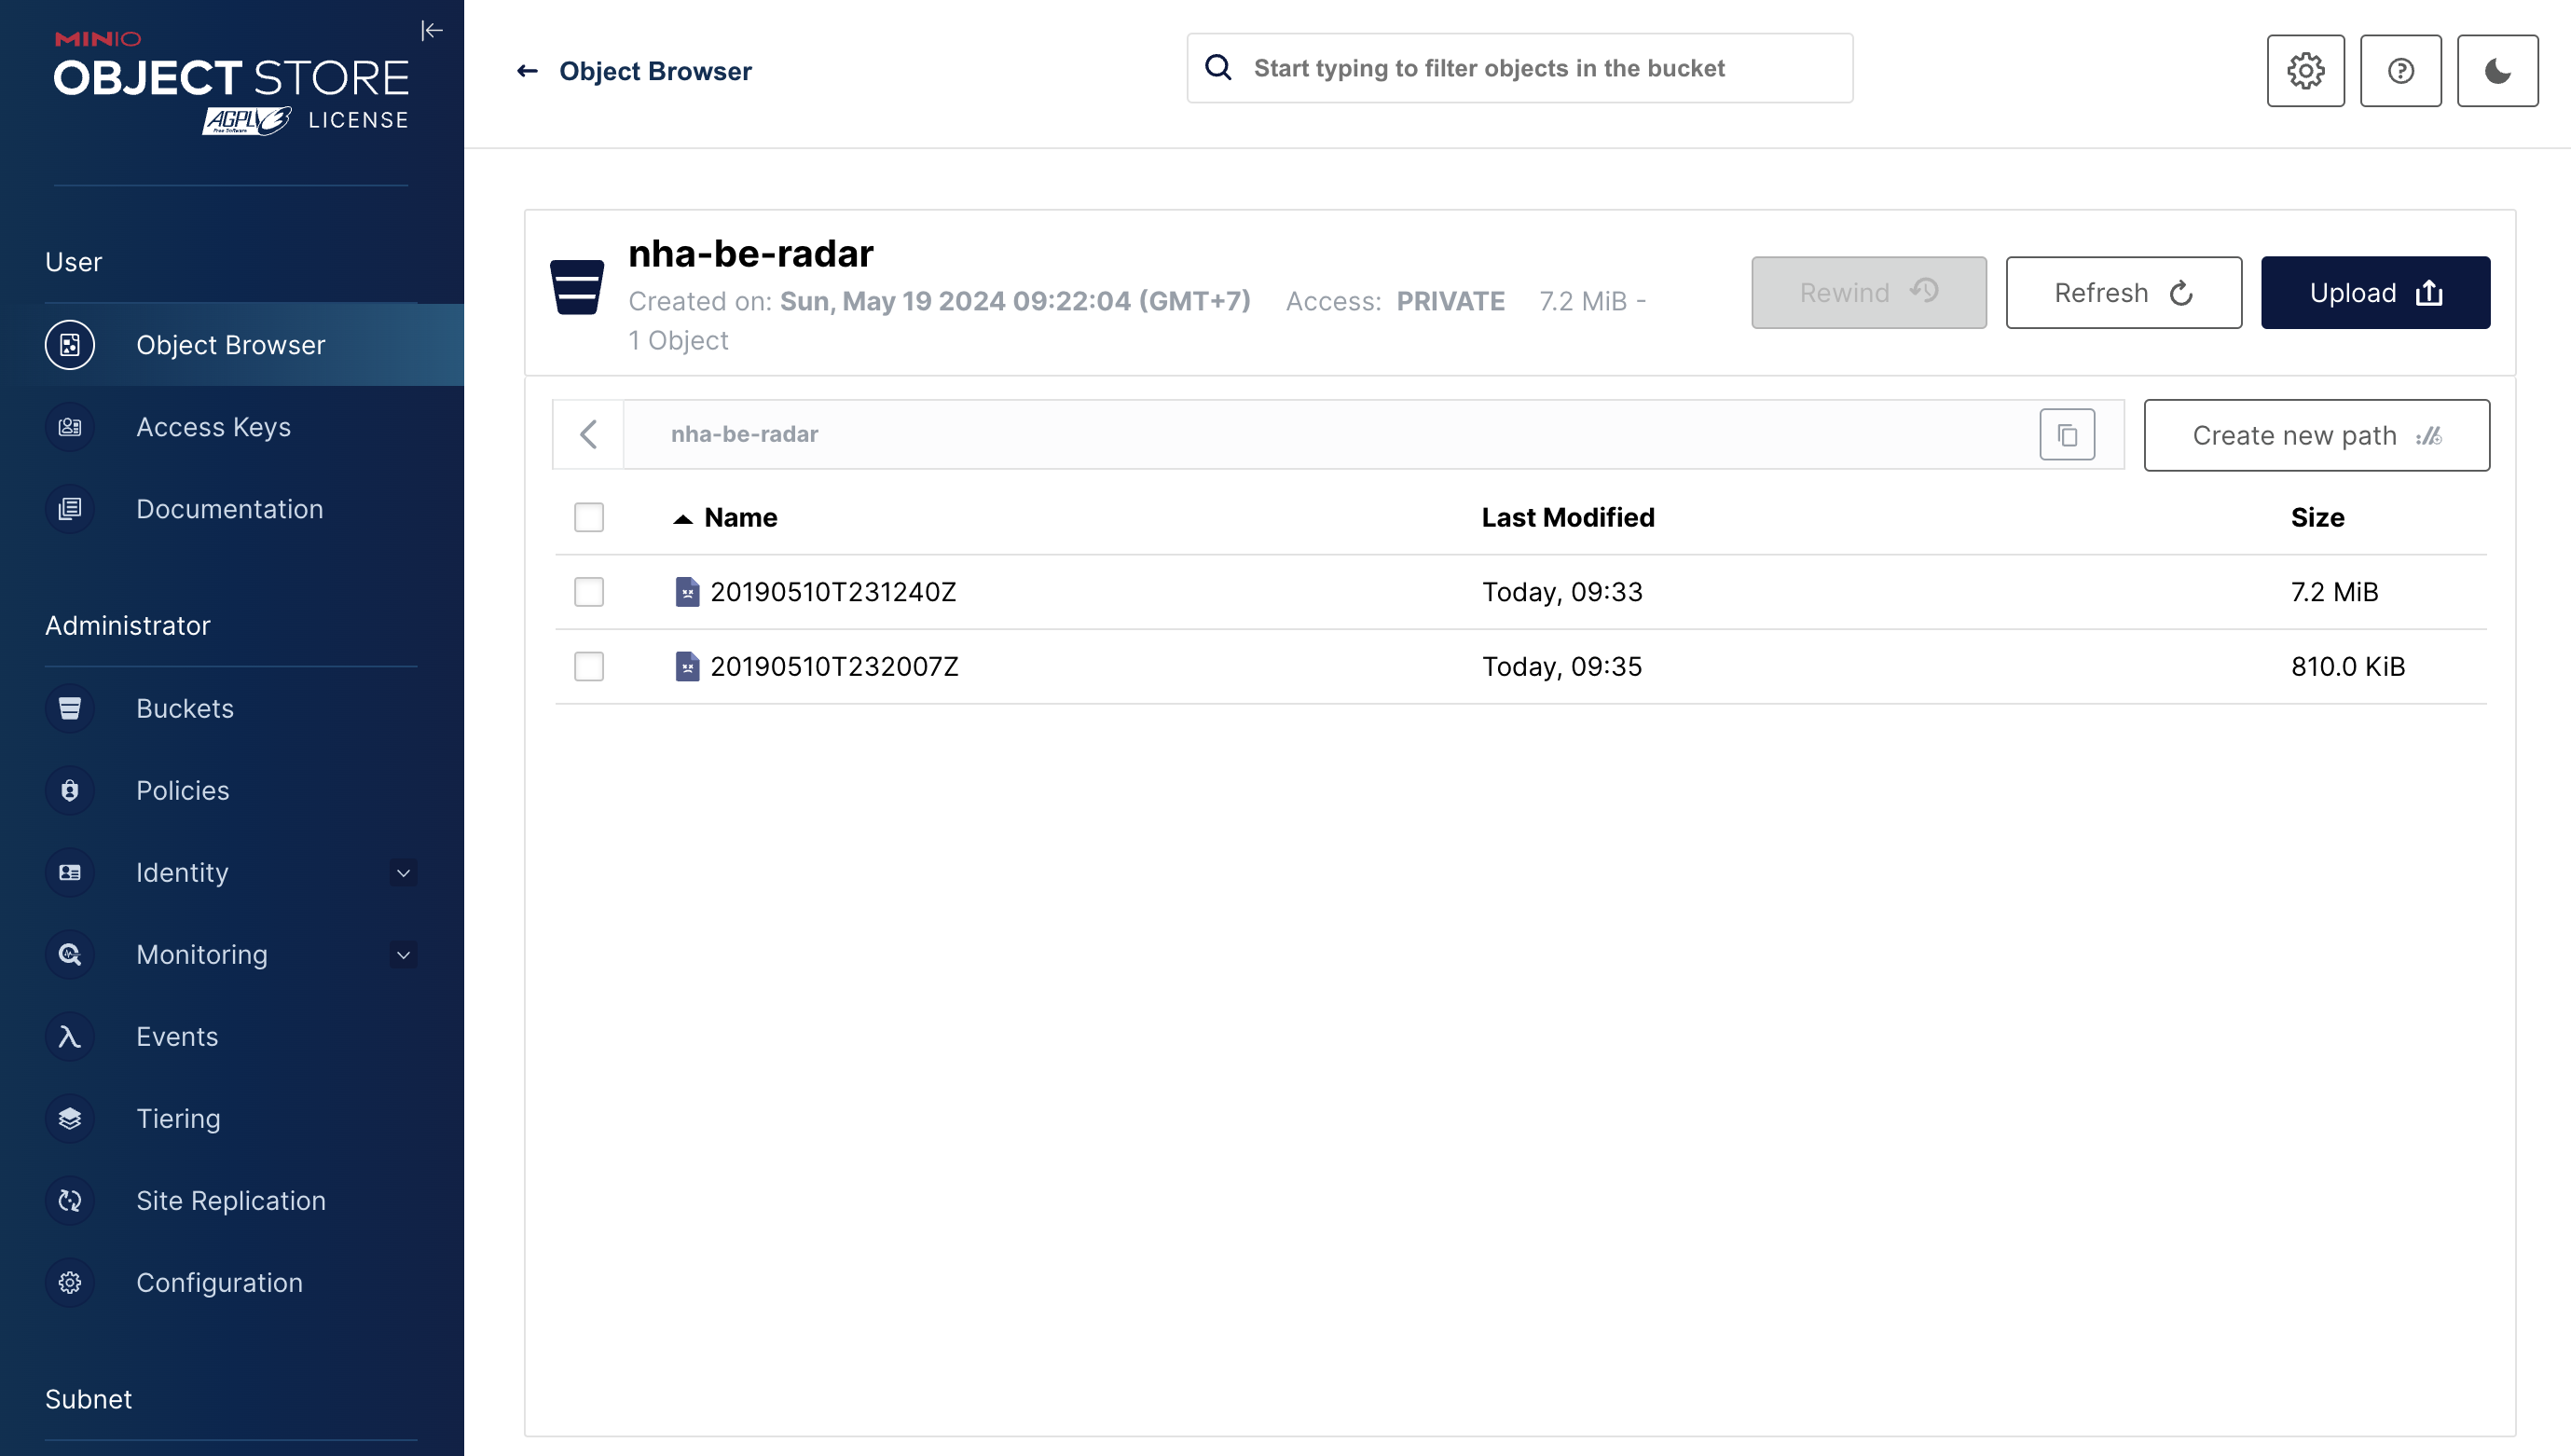
\includegraphics[width=0.8\linewidth]{Images/4.3-datastore/minio-files.png}
    \vspace{1em}
    \caption{Some radar files are currently being stored on the storage}
    \label{fig:minio-files}
\end{figure}


Not stopping at that, our system can also work with any other S3-compatible
client. One notable example of this is Cyberduck. In the future, our team can
research for more compatible protocols, such as FTP or SFTP.

\begin{figure}[H]
    \centering
    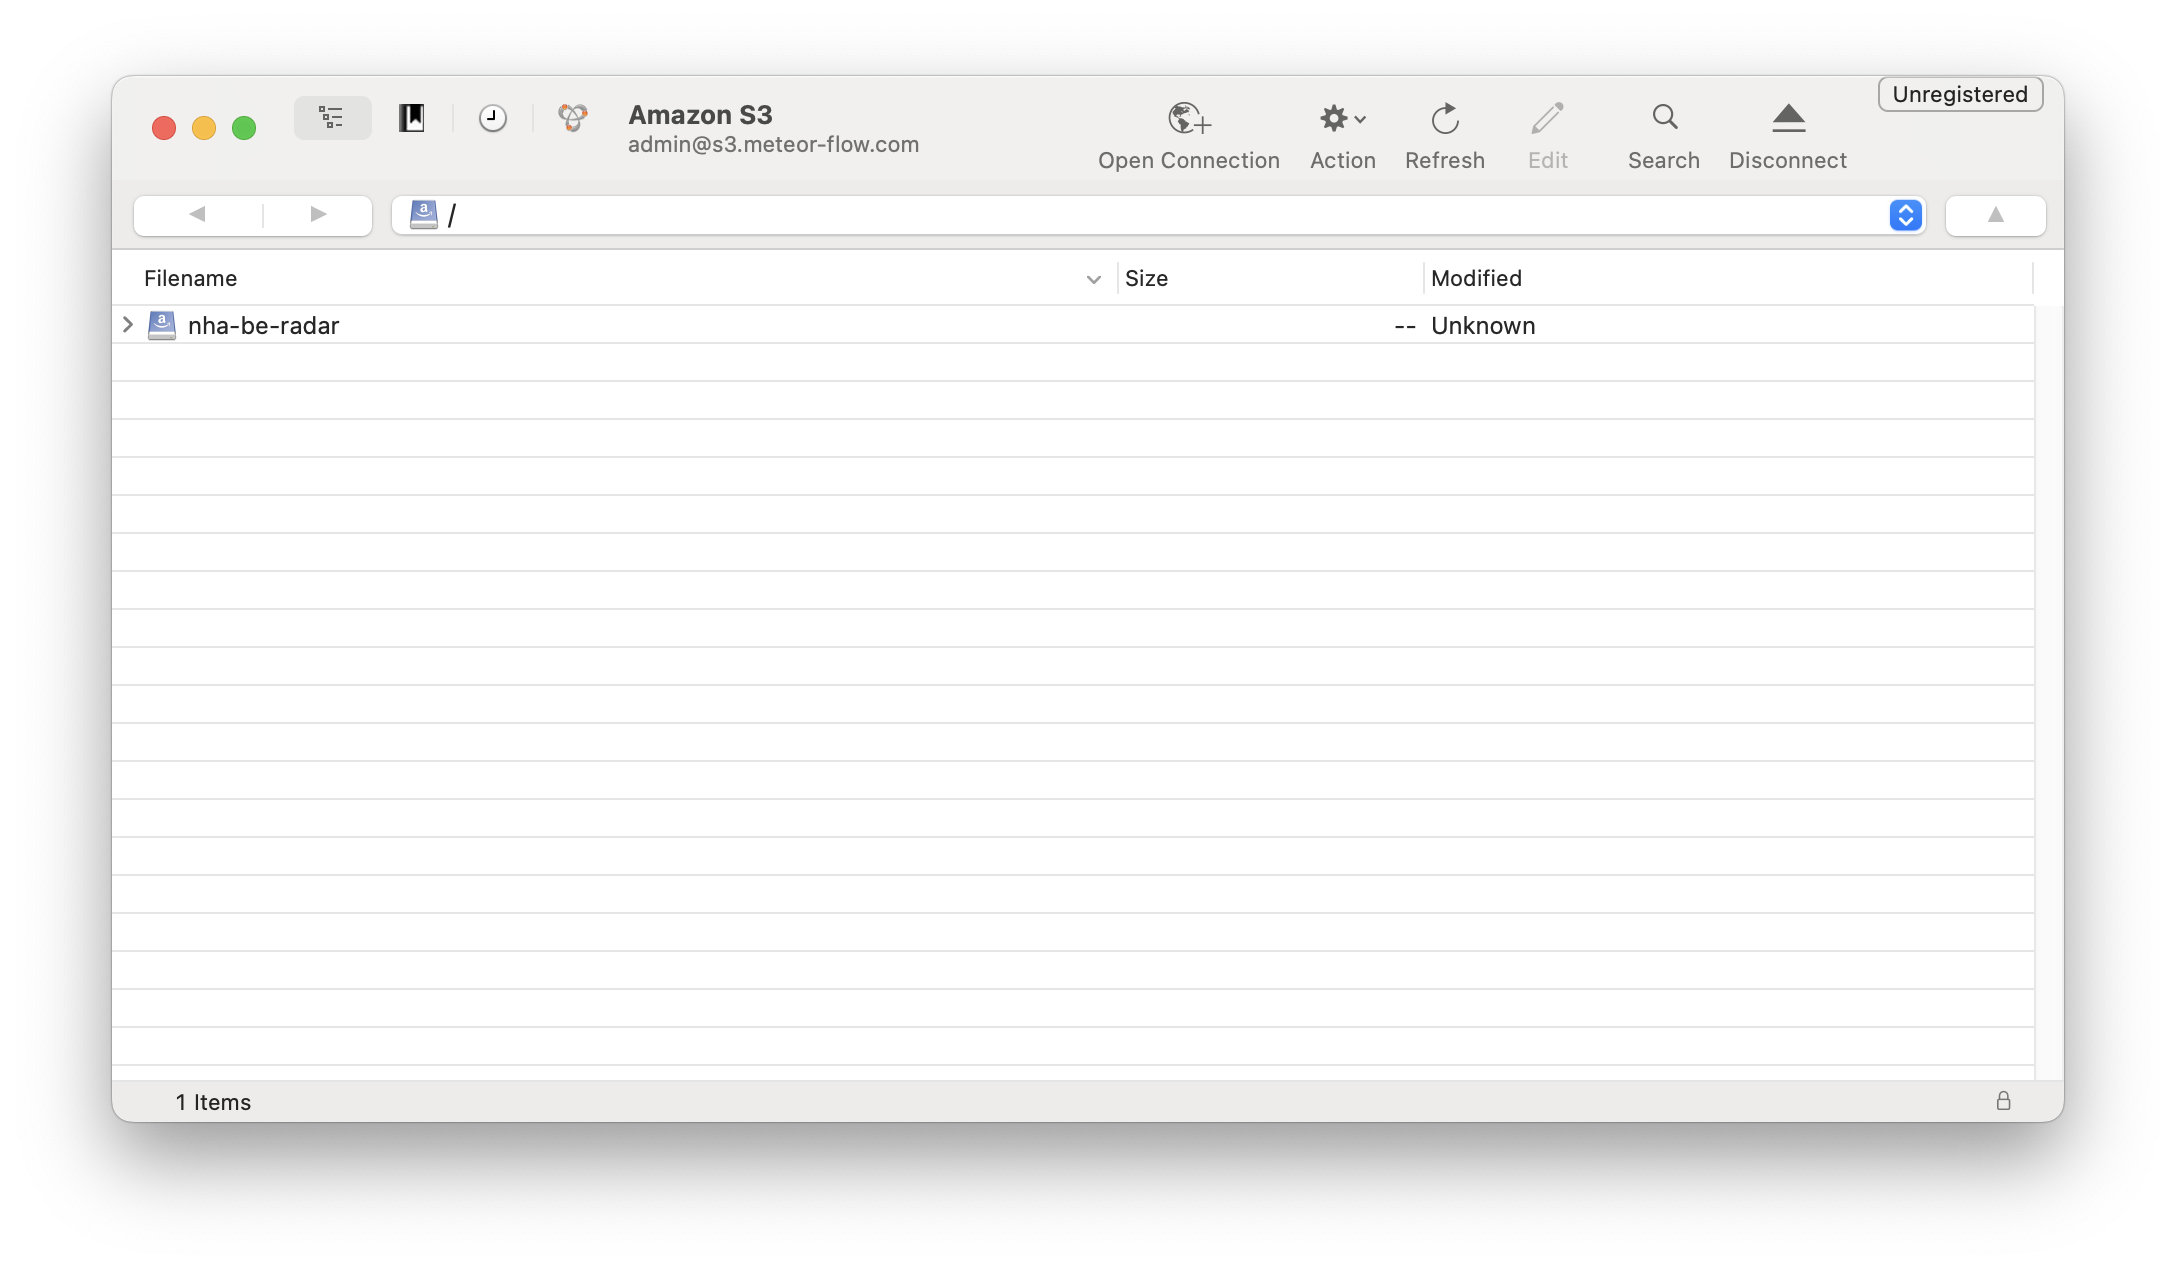
\includegraphics[width=0.6\linewidth]{Images/4.3-datastore/s3-client.png}
    \vspace{1em}
    \caption{Using Cyberduck to view data on the platform}
    \label{fig:s3-client}
\end{figure}


\newpage
\chapter{Evaluation}
\section{Functionality}

\subsection{Object Storage and data preprocessing}
The current status of our project involves the establishment of a rudimentary
data lake infrastructure, meticulously crafted using robust and efficient
Raspberry Pi servers. This infrastructure serves as the bedrock upon which we
have meticulously implemented several essential features, akin to those
prevalent in established data lake systems.

Foremost among these features is the implementation of a versatile gateway,
meticulously designed to seamlessly ingest data from an array of incoming
sources, ranging from radars to sensors. This gateway boasts compatibility with
the Amazon Web Service S3-compatible API, rendering it universally accessible to
clients and libraries engineered to interface with such protocols. Its
compatibility with this widely adopted standard ensures that our gateway can
seamlessly integrate with a plethora of external sources, thus enhancing the
scalability and versatility of our infrastructure manifold.

Moreover, a robust platform for Data Orchestration has been deployed, with
Apache Airflow serves as its cornerstone. This strategic implementation not
only streamlines the current data management processes but also lays a solid
foundation for the future scalability and expansion of our system. By
orchestrating the scheduling, monitoring, and reporting of all data flows within
the ecosystem, Airflow ensures the seamless integration of new tenants and
providers, thereby safeguarding the integrity and efficiency of our data
management operations.

In addition to these pivotal components, our team has diligently developed and
published PyTorch's native Data Loader to PyPI, a renowned package management
platform within the Python developer community. This initiative represents a
significant milestone in our endeavor to streamline data access and utilization
within our ecosystem. By providing researchers with a user-friendly library that
abstracts the complexities of low-level API interactions, we aim to
significantly reduce the learning curve associated with navigating our data lake
infrastructure. This strategic move not only enhances the accessibility of our
system but also fosters a conducive environment for innovation and collaboration
within the research community.

\subsection{Partial integration with data model team}

Upon deployment, the system will serve as a conduit for the data model team,
facilitating streamlined access to requisite data and expediting the
commencement of their model training endeavors. The seamless integration of the
system mitigates the exigency of laborious manual file management tasks,
alleviating researchers' cognitive load and empowering them to direct their
attention towards crucial aspects such as delineating pertinent regions,
identifying essential features, and scrutinizing related fields pivotal for the
fulfillment of their duties. This strategic reallocation of focus engenders a
more efficacious research workflow, wherein scholars can devote their cognitive
resources towards analytical tasks rather than being ensnared by administrative
overheads.

\begin{figure}[H]
    \centering
    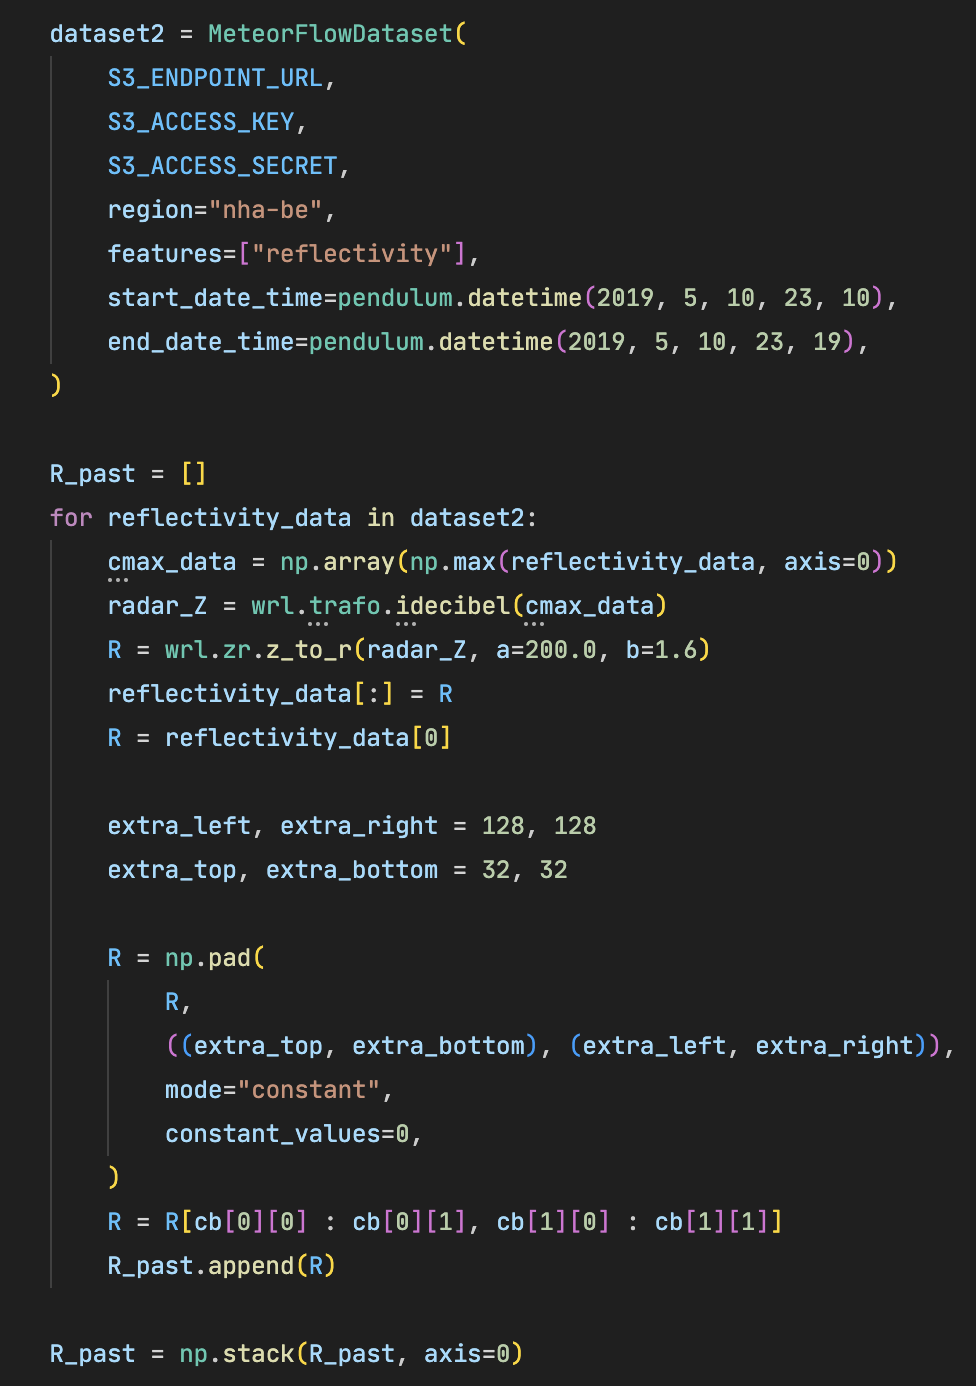
\includegraphics[width=0.8\linewidth]{Images/5-data-model-loader.png}
    \vspace{1cm}
    \caption{Part of code used by the data model team using our system}
    \label{fig:data-model}
\end{figure}

Furthermore, the system's capacity to automate the retrieval and processing of
data engenders a paradigm shift in research methodologies, fostering a more
data-centric approach characterized by enhanced efficiency and efficacy. By
obviating the need for researchers to expend time and effort on mundane data
handling tasks, the system engenders a conducive environment for scholarly
inquiry wherein investigators can delve deeper into data analysis, hypothesis
testing, and model refinement. Consequently, this augments the pace of
scientific inquiry, catalyzing the exploration of complex phenomena and
expediting the generation of novel insights that underpin advancements across
diverse domains.


\subsection{Form Builder and advanced features}
The integration of the Form Builder as an add-on feature represents a strategic
enhancement tailored to cater to the specific needs of our discerning customer
base. Stemming from insights garnered during a comprehensive field trip to the
Nha Be radar station, our team identified an opportunity to streamline and
augment the operational workflow of operators tasked with responding to
hazardous weather conditions. In response to this pressing need, we proposed and
swiftly implemented the Form Builder feature, envisaging it as a pivotal tool in
facilitating the seamless completion of warning forms amidst adverse weather
events.

The preliminary implementation of the Building Form functionality marks an
auspicious milestone in the development trajectory of this feature. While it
remains in the nascent stages of development, we are optimistic about its
potential to address the operational inefficiencies and pain points encountered
by operators at the Nha Be radar station. By affording operators an intuitive
and user-friendly interface for form completion, we envisage a tangible
improvement in workflow efficiency and responsiveness, thereby bolstering the
station's capacity to effectively manage hazardous weather conditions.

Furthermore, beyond its immediate utility as a workflow enhancement tool, the
Form Builder feature holds promise as a source of valuable insights and data for
our team. Through the aggregation and analysis of hand-labeled data generated
during the form completion process, we anticipate gaining invaluable insights
into the operational dynamics and decision-making processes underpinning hazard
response scenarios. This rich repository of data not only informs iterative
improvements to the Form Builder feature but also serves as a springboard for
enhancing our understanding of user needs and preferences, thereby fostering a
culture of continuous improvement and innovation within our organization.

Looking ahead, we remain steadfast in our commitment to refining and optimizing
the Form Builder feature to meet the evolving needs and expectations of our
stakeholders. Through ongoing collaboration and feedback from end-users, we
endeavor to iteratively enhance the functionality and usability of this feature,
ensuring its seamless integration into the operational workflows of operators at
the Nha Be radar station. Moreover, we remain vigilant in our efforts to
leverage the insights gleaned from this initiative to inform future product
development endeavors, thereby solidifying our position as a trusted provider of
innovative solutions tailored to the unique challenges of weather hazard
response.


\section{Performance Evaluation}
Following the meticulous execution of rigorous load tests conducted on our
self-hosted servers, we are pleased to present an insightful overview of the
results obtained. Despite the deployment of our system on Raspberry Pi servers,
it is imperative to underscore that this architectural choice has had minimal
impact on the overarching efficiency and performance of our solution, as
elucidated by the findings of our comprehensive assessment.

Upon subjecting our infrastructure to intensive load-testing scenarios, we
observed a commendable level of resilience and stability exhibited by our
Raspberry Pi-based servers. Contrary to preconceived notions regarding the
limitations of such hardware configurations, our empirical data revealed that
the performance metrics remained within acceptable thresholds, thereby affirming
the viability of our chosen infrastructure for hosting data-intensive
applications.

Furthermore, our meticulous analysis unearthed nuanced insights into the
intricate dynamics governing the performance characteristics of our system.
Leveraging sophisticated monitoring tools and methodologies, we meticulously
scrutinized various performance parameters, ranging from CPU utilization and
memory allocation to network throughput and latency. Through this meticulous
examination, we gleaned a comprehensive understanding of the underlying factors
influencing the efficiency of our infrastructure, thereby empowering us to
optimize and fine-tune our system for enhanced performance and scalability.

\subsection{Machine specification}

Below delineate several intricacies concerning the cluster implemented for
experimental evaluation. These facets collectively denote the comprehensive
configuration and functionalities of the cluster, delineating its capacity,
performance benchmarks, and compatibility with diverse computational tasks.

\begin{table}[H]
    \centering
    \begin{tabular}{|l|l|l|}
        \hline
        \rowcolor[HTML]{C0C0C0}
        Specification & Details                                                                                                   & Note                \\ \hline
        Server        & Raspberry Pi 3B+                                                                                          & deploying 2 servers \\ \hline
        CPU           & \begin{tabular}[c]{@{}l@{}}Broadcom BCM2837B0, \\ quad-core A53 (ARMv8)\\ 64-bit SoC @1.4GHz\end{tabular} & each                \\ \hline
        RAM           & 1GB LPDDR2 SDRAM                                                                                          & each                \\ \hline
        Disk          & 16GB + 32GB                                                                                               &                     \\ \hline
        Ethernet      & 80 Mbps                                                                                                   & total               \\ \hline
    \end{tabular}
\end{table}


\subsection{Writing large volume of data}

To rigorously evaluate the ingestion capabilities of our system, our team
embarked on a meticulous testing regimen, leveraging the S3 interface for
uploading Nha Be SIGMET files. Employing the Cyberduck client as our preferred
tool for interfacing with the S3 protocol, we systematically endeavored to
ascertain the system's ability to seamlessly ingest a substantial volume of
data. The empirical findings gleaned from these rigorous tests furnish
invaluable insights into the scalability and robustness of our infrastructure,
thereby informing strategic decisions about its optimization and enhancement.

During our testing endeavors, we observed that the system demonstrated
commendable resilience and efficiency, steadfastly accommodating the ingestion
of up to 18 files in a single upload operation. While this threshold remained
consistent across multiple test iterations, it is noteworthy that on certain
occasions, our system exhibited heightened performance, facilitating the
ingestion of approximately 25 files, with a cumulative size approximating 100
MB. This variability underscores the dynamic nature of our system's ingest
capabilities, with performance metrics fluctuating in response to diverse
environmental factors and operational parameters.

\begin{figure}[H]
    \centering
    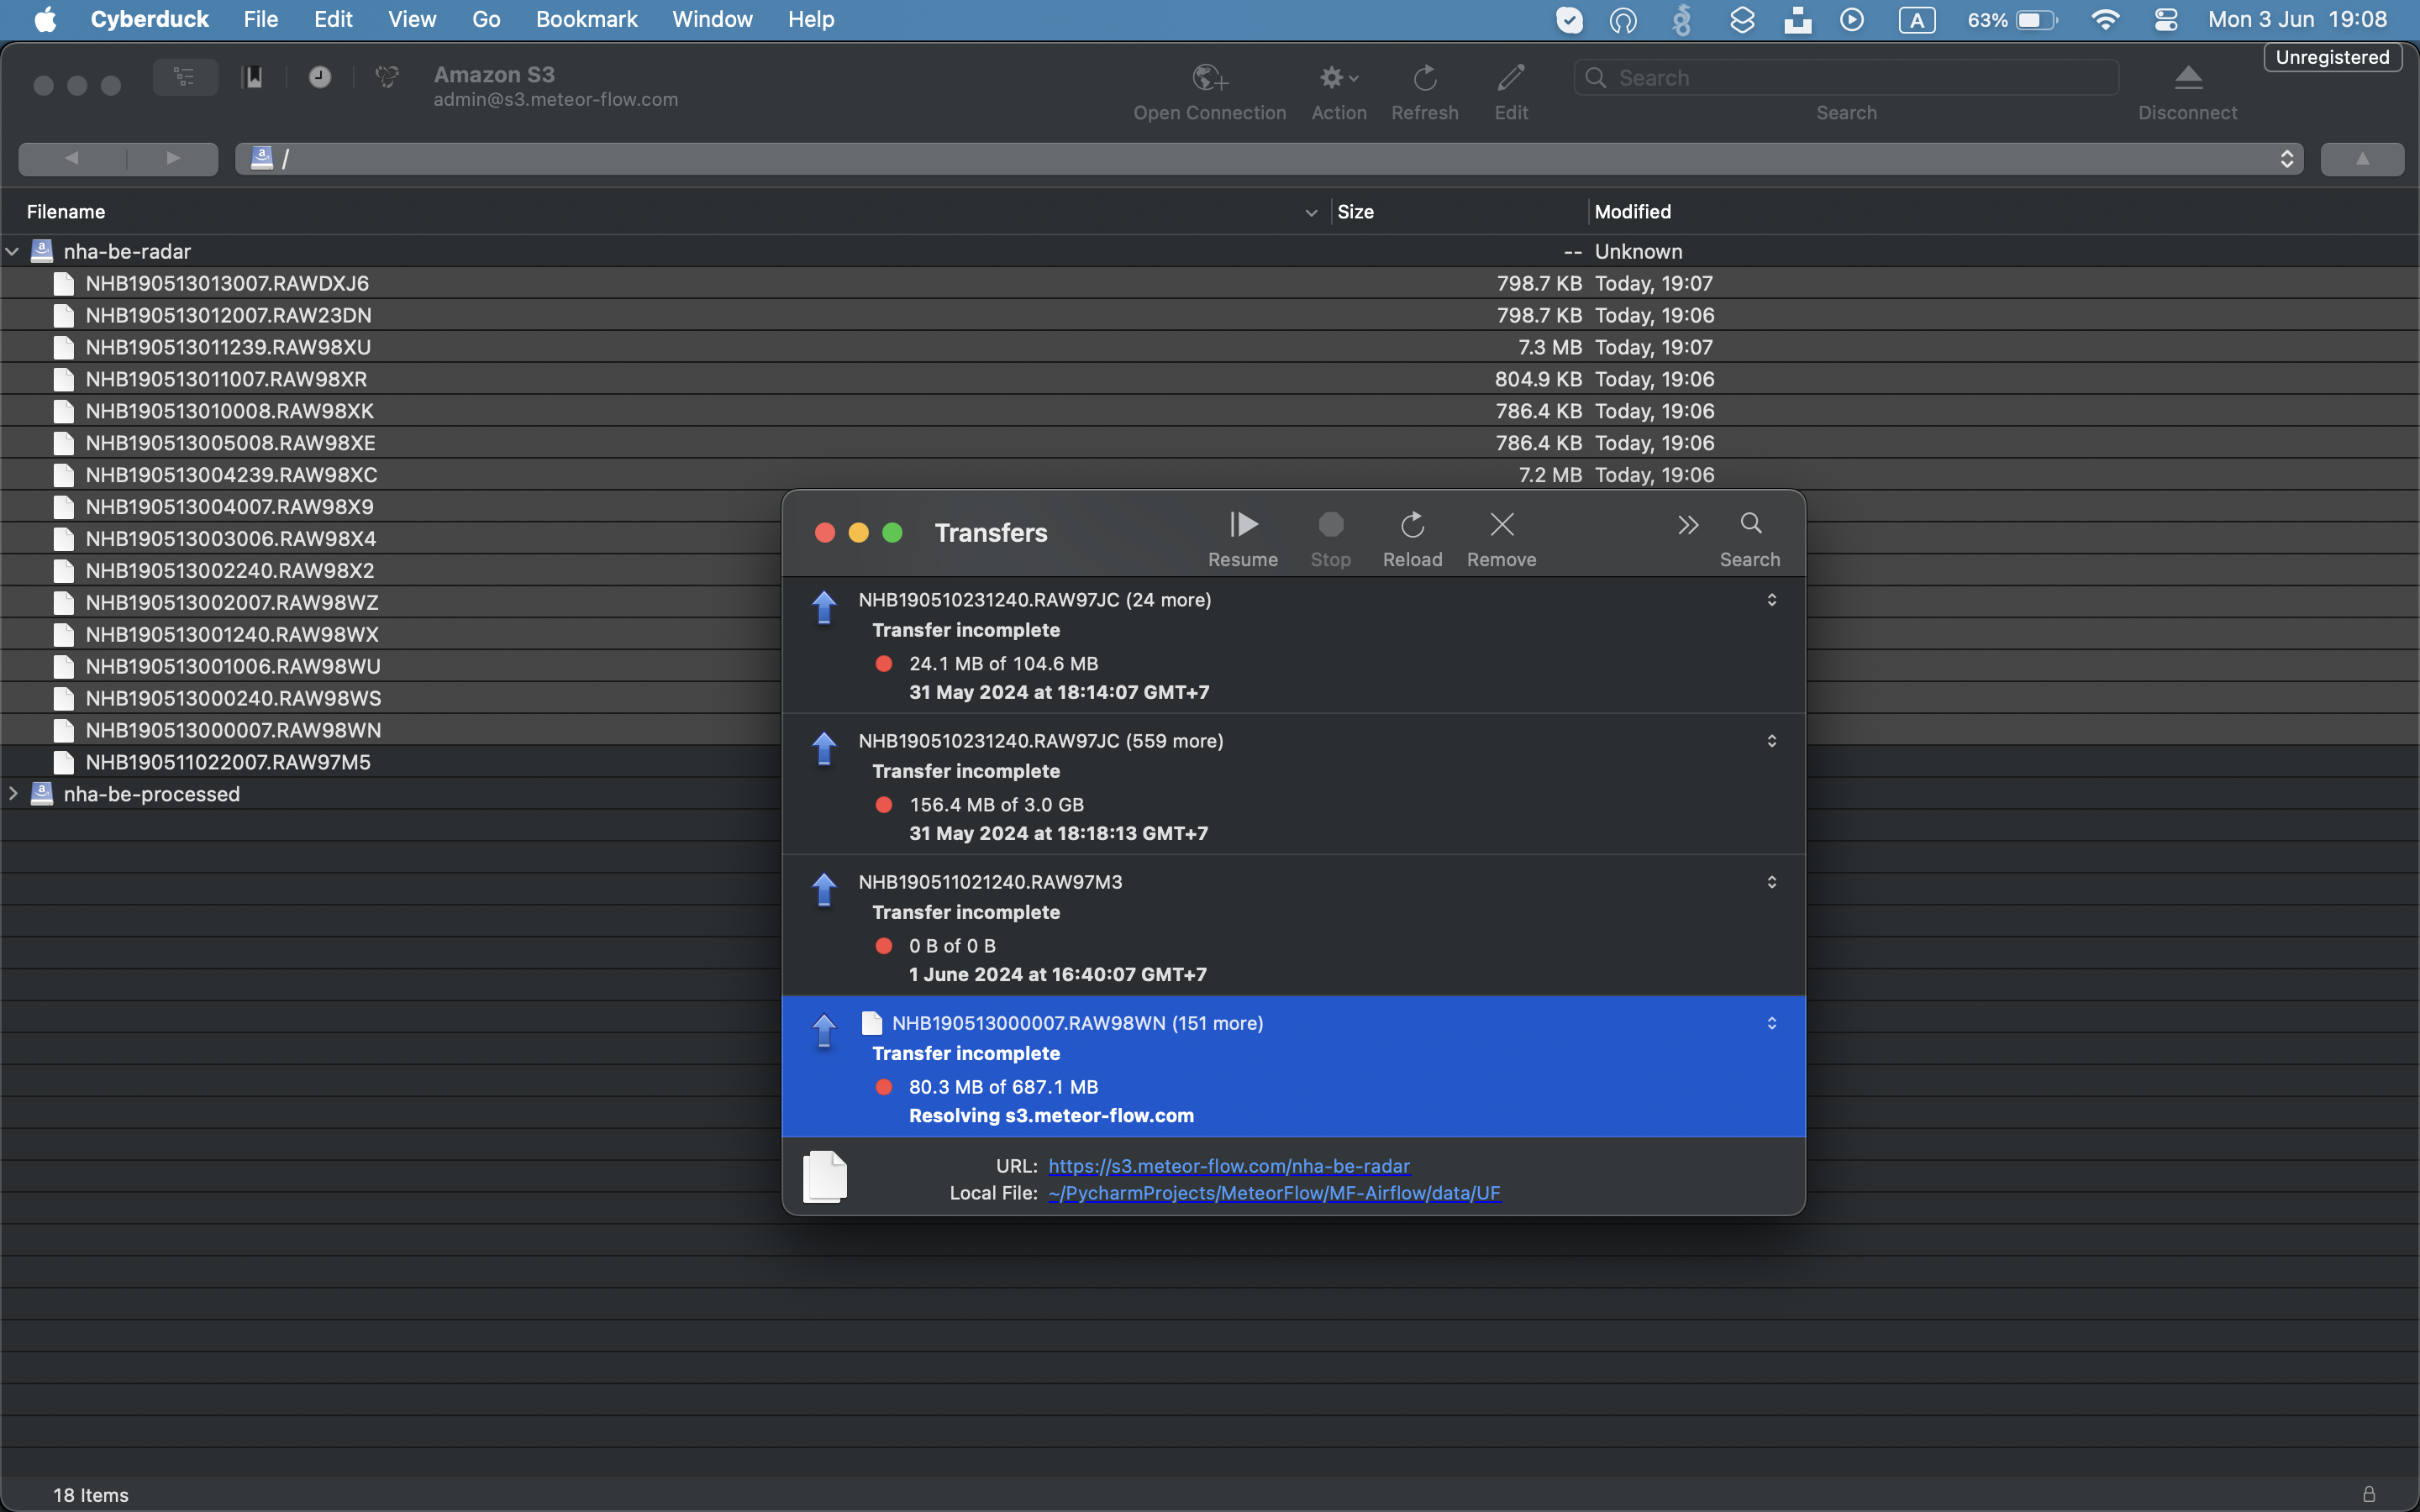
\includegraphics[width=0.8\linewidth]{Images/5-upload-18-files.png}
    \vspace{1cm}
    \caption{Writing files in bulk}
    \label{fig:bulk-write}
\end{figure}

Furthermore, it is imperative to contextualize these empirical findings within
the broader framework of real-world data acquisition scenarios. Notably, the Nha
Be radar generates meteorological data at a frequency of one scan every 10
minutes, thereby necessitating a robust infrastructure capable of seamlessly
handling the influx of data streams from disparate sources. Our empirical
analysis revealed that our system is adept at managing up to 10 concurrent
streams of incoming data, thus affirming its suitability for accommodating the
diverse needs of tenants seeking to integrate with our ecosystem.

Moreover, it is essential to underscore the significance of these findings in
the context of resource optimization and infrastructure scalability. Despite
operating within the constraints of a low-end infrastructure, our system has
demonstrated remarkable efficacy and resilience, underscoring the potential for
leveraging cost-effective hardware solutions to achieve optimal performance
outcomes. This strategic alignment of technological resources with operational
objectives not only enhance the efficiency of our system but also augment its
scalability and adaptability in response to evolving demands and requirements.

In conclusion, the comprehensive testing regimen undertaken by our team has
yielded invaluable insights into the ingestion capabilities of our system,
shedding light on its scalability, resilience, and performance characteristics.
Through meticulous analysis and optimization efforts, we are poised to further
enhance the efficiency and robustness of our infrastructure, thereby laying the
groundwork for a future characterized by unparalleled innovation and excellence
in data management and processing.


\subsection{Processing data}

In pursuit of enhancing the informativeness and query efficiency of our data, as
well as mitigating loading bandwidth concerns, our team has judiciously opted to
undertake preprocessing measures on the provided files. Central to this
preprocessing strategy is the extraction of the "reflectivity" field, a pivotal
attribute within the dataset, which is subsequently stored directly as a NumPy
array. By meticulously orchestrating these preprocessing tasks within the
purview of the Apache Airflow framework, we endeavor to streamline data
manipulation processes while fostering a conducive environment for seamless data
exploration and analysis.

The adoption of Airflow as our orchestration tool necessitated a concerted
effort to optimize and customize the system to suit our specific requirements.
Given the resource-intensive nature of Airflow, the initial deployment and
configuration of a functional cluster posed a formidable challenge for our team.
However, through a collaborative endeavor characterized by heavy optimization
endeavors and meticulous customization efforts, we succeeded in overcoming these
hurdles and achieving a state of operational readiness. This transformative
journey underscored the resilience and adaptability of our team, exemplifying
our unwavering commitment to harnessing cutting-edge technologies for the
betterment of our data management ecosystem.

\begin{figure}[H]
    \centering
    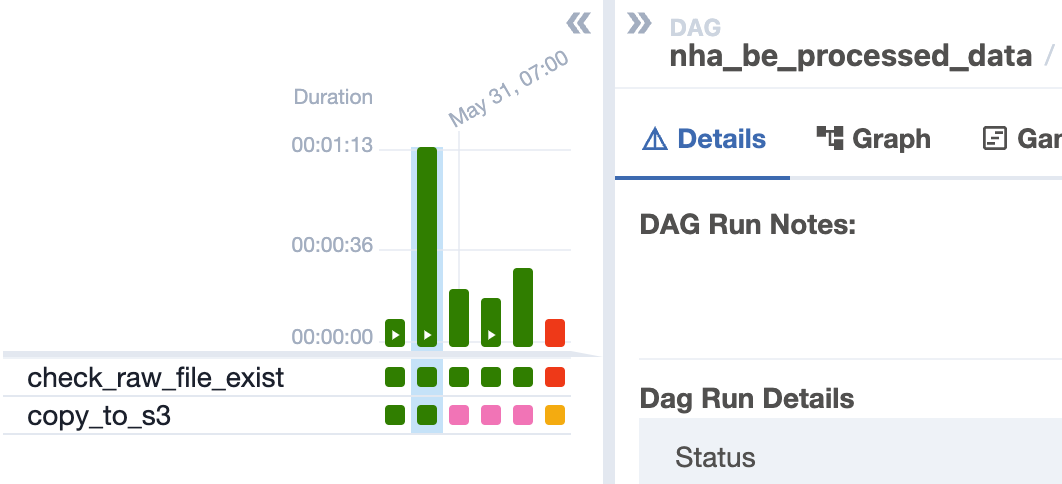
\includegraphics[width=0.8\linewidth]{Images/5-etl-data.png}
    \vspace{1cm}
    \caption{It typically takes about 1.5 minutes to process one file from Nha Be}
    \label{fig:etl-data}
\end{figure}

It is imperative to delineate the tangible outcomes of our optimization
endeavors within the broader context of operational efficiency and system
performance. By fine-tuning the configuration parameters and streamlining the
execution workflow, we have succeeded in substantially reducing the processing
latency associated with data preprocessing tasks. Empirical evidence gleaned
from extensive testing scenarios indicates that our optimized Airflow cluster
can efficiently process a batch of five files, each approximately 30 MB in size,
in less than two minutes. This remarkable feat not only underscores the efficacy
of our optimization strategies but also augurs well for the scalability and
resilience of our data processing pipeline.

\begin{figure}[H]
    \centering
    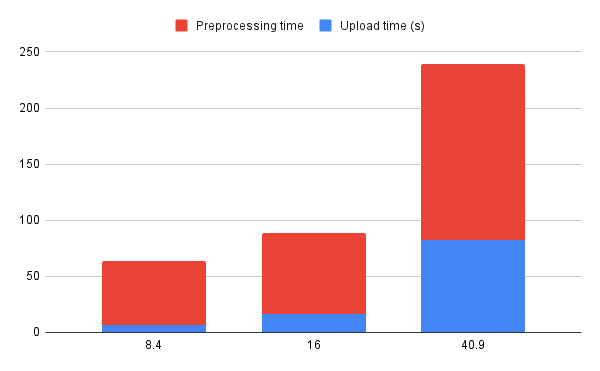
\includegraphics[width=0.8\linewidth]{Images/5-perf-chart.png}
    \vspace{1cm}
    \caption{Data upload time and preprocessing time per data size}
    \label{fig:perf-chart}
\end{figure}

Furthermore, it is essential to highlight the transformative impact of our
preprocessing efforts on the overall efficacy of our data management ecosystem.
By distilling the raw data into a concise and structured format, characterized
by the direct storage of pertinent attributes as NumPy arrays, we have
significantly enhanced the accessibility and usability of the dataset.
Researchers and analysts can now leverage these preprocessed datasets to glean
valuable insights and derive meaningful conclusions with unprecedented
efficiency and accuracy, thereby catalyzing transformative advancements across
diverse domains.


\subsection{Concurrently reading data}
Using the PyTorch API that we have implemented, we perform reading data in
multiple processes. This innovative approach not only facilitates seamless
access to our data storage but also serves as a poignant simulation of
real-world scenarios wherein disparate model teams endeavor to interact with our
comprehensive dataset.

Our empirical findings reveal that our servers exhibit commendable resilience
and efficiency in handling the influx of querying threads accessing training
data. Remarkably, our infrastructure demonstrates robust performance even under
moderate load, with the capacity to seamlessly accommodate up to 5 querying
threads without experiencing any detrimental impact on system stability or
performance. This resilience is indicative of the robustness and efficacy of
both the underlying MinIO storage system and our meticulously designed
infrastructure architecture, affirming the soundness of our technological
choices and engineering decisions.

\begin{figure}[H]
    \centering
    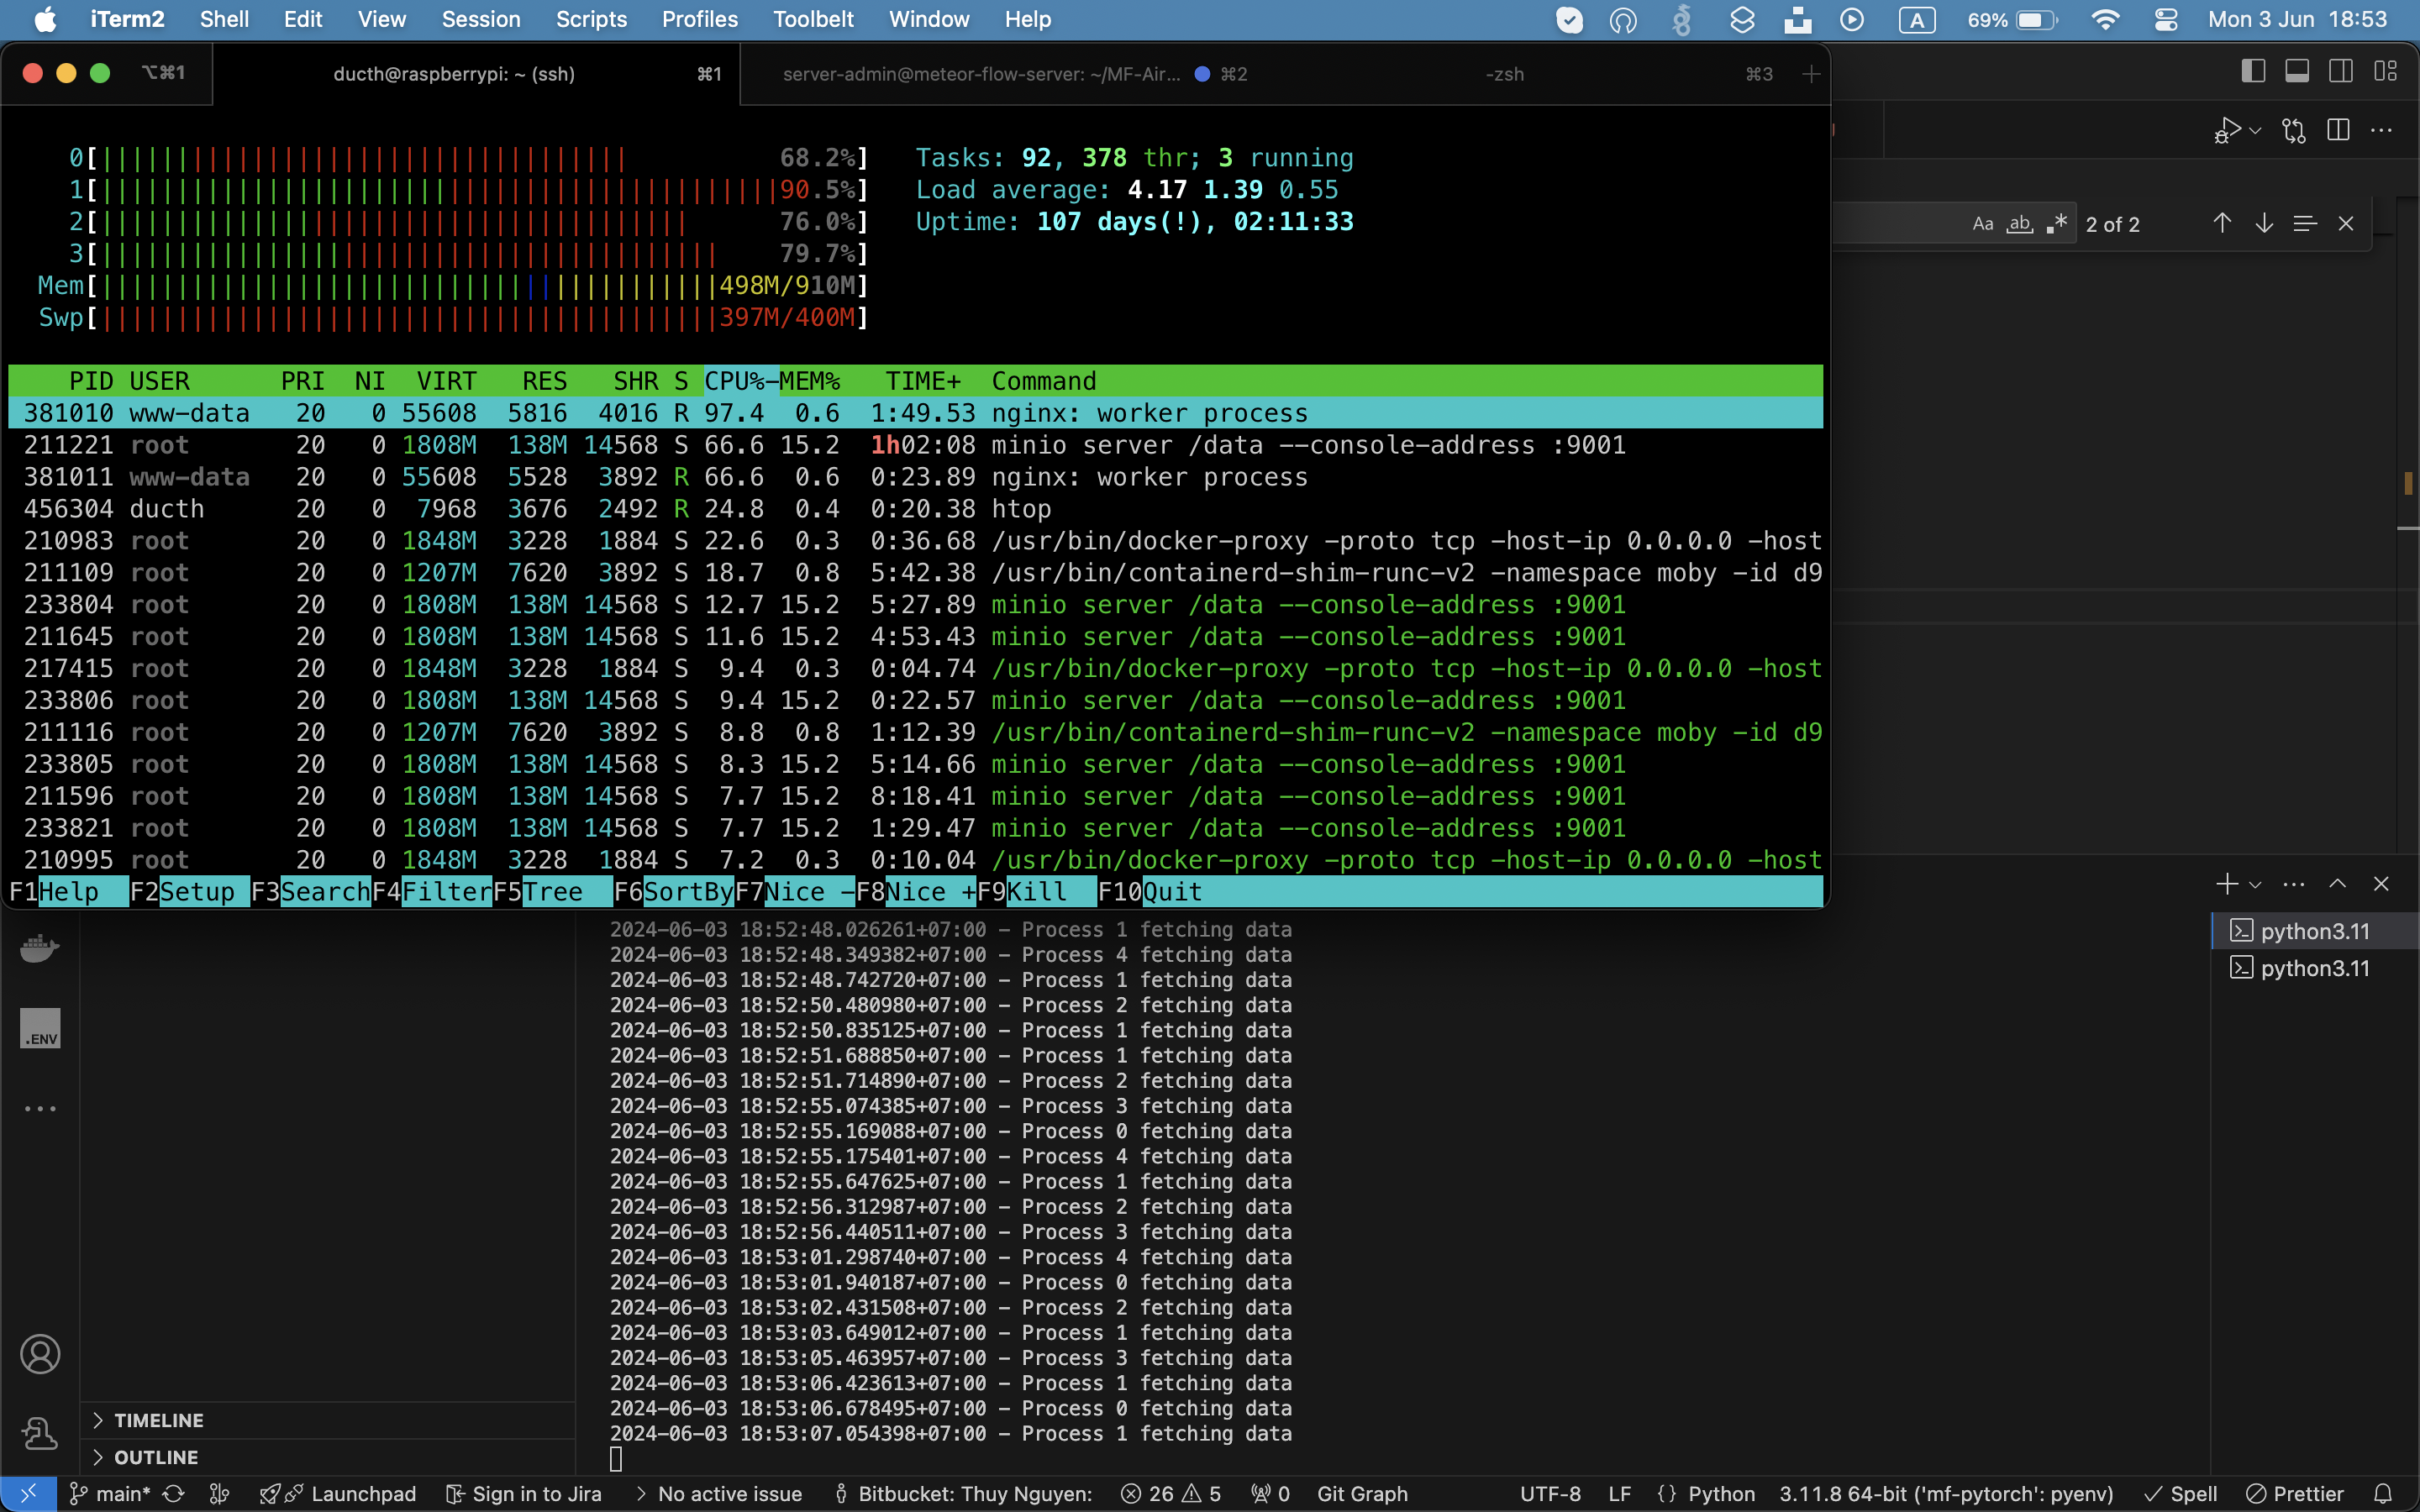
\includegraphics[width=0.8\linewidth]{Images/5-read-5-process-at-once.png}
    \vspace{1cm}
    \caption{Five concurrent thread reading data at the same time}
    \label{fig:concurrent-read}
\end{figure}

It is imperative to contextualize these empirical findings within the broader
framework of model training workflows, wherein the interplay between data
retrieval and model computation is pivotal. From a holistic perspective, the
nominal increase in load time for each batch of data retrieval can be
effectively mitigated by the inherent runtime required for model training
between successive batches. Thus, while there may be a marginal increase in
latency attributable to concurrent querying threads, this impact is mitigated by
the inherent asynchronous nature of model training workflows, thereby ensuring
optimal utilization of computational resources and minimizing potential
bottlenecks.

However, notwithstanding the commendable performance exhibited under current
testing conditions, it is prudent to exercise caution and prudence in managing
concurrent data access requests. Our empirical analysis suggests that while our
infrastructure can robustly handle up to 5 concurrent readers accessing the data
simultaneously, optimal system performance is ensured when the concurrency level
is capped at 3 readers. By imposing this constraint, we can effectively
safeguard the computational resources allocated for write operations, thereby
enhancing system stability and ensuring uninterrupted data ingestion processes.


\section{Further improvement}
In the comprehensive review of our solution, it becomes apparent that while our
system exhibits robust functionality and efficiency, there remain several areas
where additional features or enhancements could be incorporated to further
elevate its efficacy and usability. These missing features represent
opportunities for refinement and optimization, underscoring the iterative nature
of software development and the perpetual quest for excellence.

\subsection{Supports more query types on PyTorch's API}

Presently, within the framework of PyTorch's \texttt{MeteorFlowDataset}, data
retrieval capabilities are confined to querying data within a specified range or
interval of date-time parameters. For instance, users can query data pertaining
to a specific year, such as 2019, or data corresponding to particular dates,
such as the 10th and 11th of June. While this functionality suffices for basic
data retrieval tasks, the burgeoning needs of model teams necessitate the
expansion of query capabilities to encompass more sophisticated and nuanced
requirements.

To address the evolving demands for enhanced data veracity, it is imperative to
augment the existing query models with advanced functionalities that facilitate
comprehensive data exploration and analysis. Among the proposed enhancements is
the integration of support for querying data from combined areas encompassing
two or more radar stations. This strategic augmentation not only facilitates the
seamless integration of disparate data sources but also enhances the granularity
and utility of the information returned.

The implementation of advanced query models, such as querying data from combined
radar areas, represents a pivotal step towards enriching the capabilities of the
\texttt{MeteorFlowDataset} and empowering model teams with unprecedented
insights into meteorological phenomena. By enabling users to aggregate and
analyze data from multiple radar stations simultaneously, we anticipate a
quantum leap in the comprehensiveness and accuracy of the information gleaned
from the dataset.



\subsection{Increase cluster performance}
The current deployment architecture of our system can be characterized as
adequate, albeit with room for improvement. At present, the system is hosted on
two Raspberry Pi 3B+ units, which effectively handle incoming user requests.
However, despite their reliability in meeting current demands, our team has
encountered challenges related to the intricacies of configuring and optimizing
these ARM-based servers. The process of setting up the project entails
meticulous installation of various configurations tailored specifically for
these hardware platforms, often consuming significant time and effort, with
execution times stretching over hours.

While the Raspberry Pi 3B+ units have served as dependable hosts for our
services thus far, there is a palpable sense within our team of the limitations
posed by their performance capabilities. As we strive for continuous improvement
and scalability, it is imperative to explore alternatives that offer greater
computational power and flexibility. Consequently, we envision conducting
extensive research into the feasibility of transitioning to a more robust server
solutions, such as Intel NUCs or basic PCs. By leveraging these
higher-performance hardware platforms, we anticipate a significant enhancement
in our system's capabilities, enabling us to seamlessly accommodate the
anticipated growth in clusters and user base as we integrate with new tenants
and systems.

The envisioned migration to more powerful server hardware represents a strategic
investment in the future scalability and resilience of our infrastructure.
Beyond the immediate benefits of enhanced computational capabilities and
streamlined maintenance workflows, this transition holds the promise of
positioning our system on a trajectory of sustained growth and innovation. With
the agility and versatility afforded by higher-performance server solutions, we
can confidently navigate the evolving landscape of data management and
processing, ensuring seamless integration with emerging technologies and
accommodating the dynamic needs of our expanding user base.

Moreover, the adoption of alternative server hardware opens up avenues for
exploring novel optimization strategies and performance enhancements. By
capitalizing on the inherent strengths of Intel NUCs or basic PCs, we can unlock
new possibilities for fine-tuning our system architecture and streamlining
resource utilization. This strategic alignment of hardware capabilities with
operational objectives underscores our commitment to continuous improvement and
innovation, fostering a culture of excellence and resilience within our
organization.

\newpage
\chapter{Conclusion}
The Weather Data Platform (WDP) is developed to become a comprehensive solution for harnessing the power of weather data. The system is designed to meet the specific requirements of meteorologists, scholars, academic researchers, and developers from various fields, including freelancers, businesses, and Non-governmental Organizations (NGOs). WDP serves as a centralized hub for integrating weather data, analysis, and various features.

With the desire to evolve into a Weather Data Platform, we aim for the perfection and diversification of weather information. Not just a data table but a comprehensive experience. In the future, in addition to continuing to build the proposed integrated database, we promise to further research to expand and develop this integrated database into a weather data platform with the following development directions:
\begin{enumerate}
    %\item Use Software Development Life Cycle (SDLC) methods like Agile to efficiently develop and deliver the product.
    %\item Differentiate between core and extended features.
    %\item Decide whether the product should be fixed or expandable.
    %\item Monitor and adopt new technologies in the weather and forecasting field to improve data quality and predictions.
    \item \textbf{Non-linear Data:} Expand beyond basic data integration, focusing on providing non-linear, detailed, and multi-source data to help users explore more about the surrounding environment.
    \item \textbf{Artificial Intelligence Understanding:} Use artificial intelligence to understand the language of weather, from minor changes to major events, creating a deep and intelligent weather information source.
    \item \textbf{Interactive User Interface:} Not just accessing information but also interacting with weather forecasts. The user interface will be where users express curiosity and interact directly with the data.
    \item \textbf{Geospatial Information Connection:} Leverage geographical information systems to provide a contextualized, localized view of weather forecasts. This helps users understand the impact of weather on their surroundings.
          %\item Build an integrated weather data, analysis, and other data sources platform.
    \item \textbf{Performance Optimization:} Ensure quick and consistent responsiveness under all conditions.
    \item \textbf{Data Security:} Enhance data security to ensure the security and integrity of weather information.
    \item \textbf{Advanced Forecasting System:} Research and integrate artificial intelligence to improve forecasting capabilities and provide accurate forecast information.
    \item \textbf{Testing and Optimization:} Conduct system testing to ensure stability and address any potential issues. Optimize performance if necessary.
    \item \textbf{Deployment and Maintenance:} Deploy the system and maintain a regular update cycle to ensure that it consistently delivers accurate and reliable weather information.
\end{enumerate}
In this study, we have successfully built a Proof-of-Concept with high applicability, aiming to streamline the steps in the conventional workflow.
This is a crucial step towards optimizing and enhancing operational efficiency in both research and practical contexts.

Our goal was to create a flexible system with high adaptability, helping to simplify complex steps in the workflow.
In doing so, we not only contribute to increasing efficiency but also alleviate the workload pressure on personnel, creating favorable conditions for creativity and focus on core tasks.

We didn't just stop at developing the system but also proposed flexible deployment strategies, emphasizing easy integration into the current working environment of those involved in information gathering and weather forecasting tasks.



\bibliographystyle{plainnat}
\bibliography{refs}

\end{document}